\documentclass[a4paper,12pt,oneside]{jex}

\renewcommand{\baselinestretch}{1.1}
\setlength{\textwidth}{16cm}
\setlength{\textheight}{24cm}
\setlength{\evensidemargin}{0cm}
\setlength{\oddsidemargin}{0cm}
\setlength{\topmargin}{-1.0cm}

\usepackage[dvipdfmx]{graphicx}
\usepackage[dvipdfmx]{xcolor}
\usepackage[cmex10]{amsmath}
\usepackage[deluxe]{otf}
\usepackage{booktabs}
\usepackage{ascmac}
\usepackage{amssymb}
\usepackage{caption}
\usepackage{colortbl}
\usepackage{float} 
\usepackage{textcomp}
\usepackage{url}
\usepackage{multirow,multicol}
\usepackage{wrapfig}
\usepackage{listings,jvlisting} 

\usepackage{dirtree}

\西暦

\captionsetup{format=hang}
\lstset{
  basicstyle={\ttfamily\small},
  identifierstyle={\small},
  commentstyle={\small\itshape\color{gray}},
  keywordstyle={\small\bfseries\color{blue}},
  stringstyle={\small\ttfamily\color{brown}},
  showstringspaces=false,
  frame={tb},
  breaklines=true,
  columns=[l]{fullflexible},
  numbers=left,
  numberstyle={\scriptsize},
  stepnumber=1,
  numbersep=1zw,
  lineskip=-0.5ex
}
\renewcommand{\lstlistingname}{ソースコード}

\makeatletter
    \let\l@chapter@x=\l@chapter
    \def\l@chapter#1#2{\l@chapter@x{#1}\@empty}
\makeatother

\pagestyle{headings}
%\iffalse
\title{
  \bfseries\vskip30pt
  Webプログラミング　レポート課題\\
  \vspace{1cm}
}

\author{
  \\
  GitHubリンク
  \\
  \url{https://github.com/Kuro-aletta/webpro_06}
  \\
  \vspace{.5cm}
}

\date{
  \bfseries\Large\vskip10pt
  {\hspace{2cm}}学生番号 \underline{\makebox[8cm][c]{25G1020}} \vskip50pt
  {\hspace{2cm}}氏{\hspace{2em}}名 \underline{\makebox[8cm][c]{薄井　悠希}} \vskip20pt
}
%\fi
\begin{document}
%\iffalse
\maketitle
\thispagestyle{empty}
\setcounter{tocdepth}{2}

\tableofcontents
\thispagestyle{empty}

\pagenumbering{roman}
\pagenumbering{arabic}

\clearpage
\setcounter{page}{1}
%\fi
% \input{00_tutorial}
% \chapter{ワークA：センサ回路設計}

\section{はじめに}
%% ワークAを理解した上で，目的として要約する
%%
%% （例文）
%% 本課題では～を目的とし，～の実験を行った．
%% 実験を通じて～の結果を得た．
%% それらの結果より，～であることを明らかにする．

本課題では，フォトリフレクタを用いて脈拍のような微弱な信号を検出し，
後の処理に適した信号に増幅し，ノイズ除去を行う回路の設計と実装を通じて，アナログ回路の基本を学ぶことを目的とする．
実験では，オペアンプを用いたバンドパスフィルタ付き二段反転増幅回路を設計，実装した．
実験を通じて，設計した回路が信号を増幅，不要な周波数成分を除去できることを確認し，実際の脈拍を検出し増幅した観測結果を得た．
それらの結果より，微弱なセンサ信号からノイズを除去し，必要な信号のみを増幅するフィルタ増幅回路の有効性を明らかにする．




\section{方法及び手順} 
%% ワークAで設計・実装するものを理解した上で，方法や手順に落とし込んだ
%% 形で，客観的に記述する．報告書の基準は，この報告書の記述だけで，第
%% 三者が追試をし，同様の結果を得ることできることである．必要に応じて，
%% 図，表，式を用いて，曖昧な箇所や誤解を生じにくい説明が求められる．



\subsection{原理}
本実験で用いる脈拍測定の原理と，主要な電子部品の動作原理を以下に示す．


\subsubsection{脈拍測定の原理}
本実験では，光電容積脈波法の中でも，センサを身体の表面に当てることで計測が可能な反射型の方式を用いた．
これは，指先に赤外線を照射し，心臓の拍動に伴う毛細血管の血流量の変化に応じて変化する反射光の強度を測定することで脈波を得る手法である\cite{安藤譲二1990光電式脈波計測の応用}．
血流量が多くなると光の吸収量が増加して反射光は減少し，逆に血流量が少なくなると光の吸収量が減少して反射光は増加する\cite{hertzman1938blood}．
この反射光の周期的変化を電気信号として捉えることで，脈拍を測定する．


\subsubsection{フォトリフレクタ(LBR-127HLD)}
本実験で用いるフォトリフレクタ(LBR-127HLD)は，赤外線発光ダイオードとフォトトランジスタが一つのパッケージに収められた反射型光センサである\cite{LBR-127HLD}．
LEDから照射された赤外線が指先で反射し，その光をフォトトランジスタが受光する．
フォトトランジスタは，受光した光の強度に応じてコレクタ-エミッタ間に流れる電流が変化する素子であり\cite{workA_フォトトランジスタ}，
この電流の変化を抵抗によって電圧の変化に変換することで，脈波信号を出力する．


\subsubsection{オペアンプ(LM358N)を用いた信号処理}
\paragraph{反転増幅回路}
フォトリフレクタから出力される信号は微弱であるため，オペアンプを用いた反転増幅回路によって後段の処理に適した電圧レベルまで増幅する．
反転増幅回路の増幅率 $A$ は，入力抵抗 $R_s$ と帰還抵抗 $R_f$ の比によって決まり，以下の式で表される\cite{workA_オペアンプ}．
\begin{equation}
  A = - \frac{R_f}{R_s} \label{eq:A}
\end{equation}

\paragraph{バンドパスフィルタ}
脈波の周波数はおおよそ0.5Hzから2Hz程度であるため，測定時には体動による低周波の揺らぎや，商用電源などに起因する高周波ノイズが問題となる\cite{workA_脈拍周波数}．
これらの不要な信号成分を除去するため，ハイパスフィルタとローパスフィルタを組み合わせたバンドパスフィルタを実装する．
本回路では，オペアンプを用いたアクティブフィルタを構成し，入力抵抗$R_s$と直列に接続されたコンデンサを$C_s$，帰還抵抗$R_f$と並列に接続されたコンデンサを$C_f$とすると，
下限周波数 $f_L$ と上限周波数 $f_U$ は以下の式によって決定される\cite{workA_バンドパスフィルタ}．
\begin{equation}
  f_L = \frac{1}{2\pi C_s R_s} \label{eq:f_L}
\end{equation}
\begin{equation}
  f_U = \frac{1}{2\pi C_f R_f} \label{eq:f_U}
\end{equation}




\subsection{回路設計と使用部品}
本実験で実装した回路の設計計算と，それに基づき選定した使用部品について述べる．
まず信号を増幅・フィルタリングする後段回路の設計について述べ，次に入力となる脈拍検出部の設計について述べる．


\subsubsection{バンドパスフィルタ付き二段反転増幅回路の設計}
センサから得られる微弱な信号を処理するため，バンドパスフィルタ付き二段反転増幅回路を設計した．設計仕様は以下の通りである．

\paragraph{増幅率}
全体で約+91.8倍の増幅率を得るため，一段目を-30.3倍，二段目を-3.03倍に設定した．式(\ref{eq:A})に基づき，各抵抗値を式(\ref{eq:A_1})，式(\ref{eq:A_2})ように選定した．
\begin{equation}
  A_1 = -\frac{R_2}{R_5} = -\frac{1\text{M}\Omega}{33\text{k}\Omega} \approx -30.3 \label{eq:A_1}
\end{equation}
\begin{equation}
  A_2 = -\frac{R_1}{R_6} = -\frac{100\text{k}\Omega}{33\text{k}\Omega} \approx -3.03 \label{eq:A_2}
\end{equation}
この計算に基づき，$R_1=100\text{k}\Omega$, $R_2=1\text{M}\Omega$, $R_5=R_6=33\text{k}\Omega$を選定した．

\paragraph{周波数帯域}
下限周波数 $f_L \approx 0.48$ Hz，上限周波数 $f_U \approx 16$ Hzのバンドパス特性を得るよう，式(\ref{eq:f_L})および式(\ref{eq:f_U})に基づきコンデンサを選定した．
\begin{itemize}
  \item 下限周波数($f_L$): 主に$C_3$，$R_5$と$C_4$，$R_6$のハイパスフィルタで決定される．
  $C_3$，$C_4$を$10\mu\text{F}$とすると，式(\ref{eq:low_1})および式(\ref{eq:low_2})となり，回路全体の下限周波数は約0.48Hzとなる．
  \begin{equation}
    f_{L1} = \frac{1}{2\pi R_5 C_3} = \frac{1}{2\pi \times 33\text{k}\Omega \times 10\mu\text{F}} \approx 0.48 \text{Hz} \label{eq:low_1}
  \end{equation}
  \begin{equation}
    f_{L2} = \frac{1}{2\pi R_6 C_4} = \frac{1}{2\pi \times 33\text{k}\Omega \times 10\mu\text{F}} \approx 0.48 \text{Hz} \label{eq:low_2}
  \end{equation}
  したがって，$C_3=C_4=10\mu\text{F}$を選定した．
  \item 上限周波数($f_U$): 主に$R_2$，$C_2$と$R_1$，$C_1$のローパスフィルタで決定される．
  $C_2$を$0.010\mu\text{F}$, $C_1$を$0.10\mu\text{F}$とすると，式(\ref{eq:high_1})および式(\ref{eq:high_2})となり，回路全体の上限周波数は約16Hzとなる．
  \begin{equation}
    f_{U1} = \frac{1}{2\pi R_2 C_2} = \frac{1}{2\pi \times 1\text{M}\Omega \times 0.010\mu\text{F}} \approx 16 \text{Hz} \label{eq:high_1}
  \end{equation}
  \begin{equation}
    f_{U2} = \frac{1}{2\pi R_1 C_1} = \frac{1}{2\pi \times 100\text{k}\Omega \times 0.10\mu\text{F}} \approx 16 \text{Hz} \label{eq:high_2}
  \end{equation}
  したがって，$C_2=0.010\mu\text{F}$，$C_1=0.10\mu\text{F}$を選定した．
\end{itemize}
    
\paragraph{バイアス回路}
本回路は+5Vの単電源で動作させるため，抵抗分圧によるバイアス回路を設けた．
抵抗$R_8=R_{10}=100\text{k}\Omega$と$R_7=R_9=33\text{k}\Omega$を用いて基準電圧を生成し，これを各オペアンプの非反転入力端子(+)に加えている．


\subsubsection{脈拍検出回路の設計}
増幅・フィルタ回路に入力するための信号を生成するセンサ部として，脈拍検出回路を設計した．設計仕様は以下の通りである．

\paragraph{赤外LEDの電流制限抵抗($R_3$)}
赤外LEDを適切な光量で発光させるため，電流制限抵抗 $R_3$ の値を決定した．
仕様の標準値である順方向電流 $I_F$ を20mA，その際の順方向電圧 $V_F$ を1.5Vとすると\cite{LBR-127HLD}，5V電源において必要な抵抗値は式(\ref{eq:led})より算出できる．
\begin{equation}
  R_3 = \frac{V_{CC} - V_F}{I_F} = \frac{5\text{V} - 1.5\text{V}}{20\text{mA}} = 175 \Omega \label{eq:led}
\end{equation}
本実験では，計算値の2倍弱の抵抗値として$330 \Omega$を選定した．

\paragraph{フォトトランジスタの負荷抵抗($R_4$)}
フォトトランジスタの負荷抵抗($R_4$): フォトトランジスタが受光した光の強度変化を電圧の変化に変換するため，負荷抵抗 $R_4$ の値を決定した．
フォトトランジスタに光が照射され飽和した際のコレクタ-エミッタ間飽和電圧 $V_{CE(sat)}$ を0.4V，その際のコレクタ電流 $I_C$ を2mAとすると\cite{LBR-127HLD}，
5V電源において必要な抵抗値は，式(\ref{eq:ft})より算出できる．
\begin{equation}
  R_4 = \frac{V_{CC} - V_{CE(sat)}}{I_C} = \frac{5\text{V} - 0.4\text{V}}{2\text{mA}} = 2300 \Omega \label{eq:ft}
\end{equation}
%本実験で使用可能な抵抗器のうち，計算値の2倍($1700\Omega$)に近いものは$330\Omega$と$3.3k\Omega$であった．
%ここで，$R_4$ の値は，脈波による微弱な電流変化を電圧変化に変換する感度を決定する要素であり，抵抗値が大きいほど感度は向上する．
%計算値より低い$330\Omega$では感度が不足する可能性があるため，より高い感度が得られる$3.3k \Omega$を選定した．
%これにより，脈波の微細な変化をより大きな電圧振幅として後段回路に伝えることが期待できる．
本実験では，計算値の2倍弱の抵抗値として$3.3k \Omega$を選定した．


\subsubsection{使用部品一覧}
以上の設計計算に基づき選定した部品の一覧を表\ref{tab:parts_list}にまとめる．
\begin{table}[H]
  \caption{部品表}
  \centering
  \begin{tabular}{|l|c|l|l|}
    \hline
    部品名 & 数量 & 仕様 & 素子変数 \\
    \hline \hline
    炭素皮膜抵抗 & 1 & $330 \Omega$ & $R_3$ \\
    \hline
    炭素皮膜抵抗 & 1 & $3.3k \Omega$ & $R_4$ \\
    \hline
    炭素皮膜抵抗 & 4 & $33k \Omega$ & $R_5, R_6, R_7, R_9$ \\
    \hline
    炭素皮膜抵抗 & 2 & $1M \Omega$ & $R_2, R_{11}$ \\
    \hline
    炭素皮膜抵抗 & 3 & $100k \Omega$ & $R_1, R_8, R_{10}$ \\
    \hline
    積層セラミックコンデンサ & 2 & $10 \mu F$ & $C_3, C_4$ \\
    \hline
    積層セラミックコンデンサ & 1 & $0.010 \mu F$ & $C_2$ \\
    \hline
    積層セラミックコンデンサ & 1 & $0.10 \mu F$ & $C_1$ \\
    \hline
    オペアンプ & 1 & LM358N & - \\
    \hline
    フォトリフレクタ & 1 & LBR-127HLD & - \\
    \hline
    オシロスコープ & 1 & Tektronix TBS1000C & - \\
    \hline
    波形出力デバイス & 1 & ATOM Lite & - \\
    \hline
  \end{tabular}
  \label{tab:parts_list}
\end{table}

\newpage

\subsubsection{回路図}
表\ref{tab:parts_list}から作成した回路図を図\ref{fig:1_fig}，図\ref{fig:2_fig}に示す．
図\ref{fig:1_fig}はワークA-1，図\ref{fig:2_fig}はワークA-2の回路図である．
\begin{figure}[H]
  \centering
  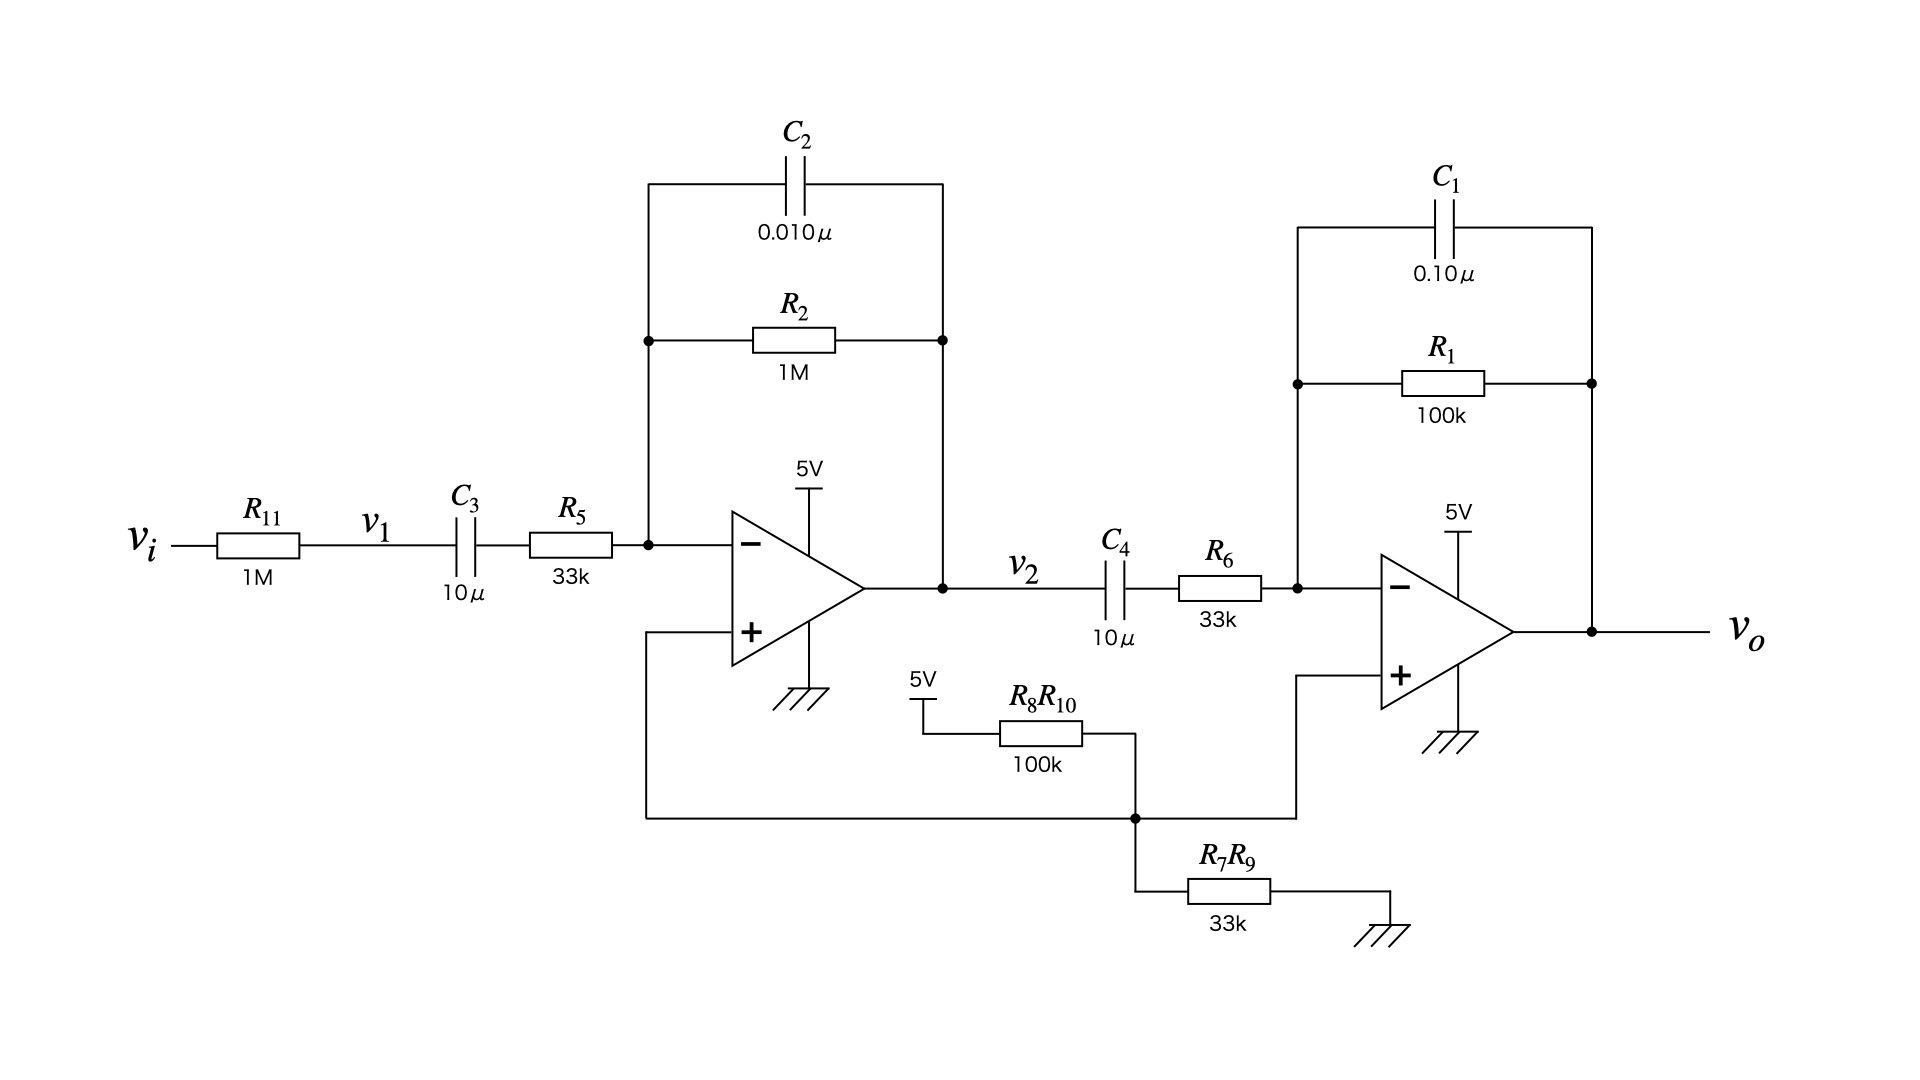
\includegraphics[width=1\linewidth]{fig_work_A/1_fig.jpg}
  \caption{ワークA-1 回路図}
  \label{fig:1_fig}
\end{figure}
\begin{figure}[H]
  \centering
  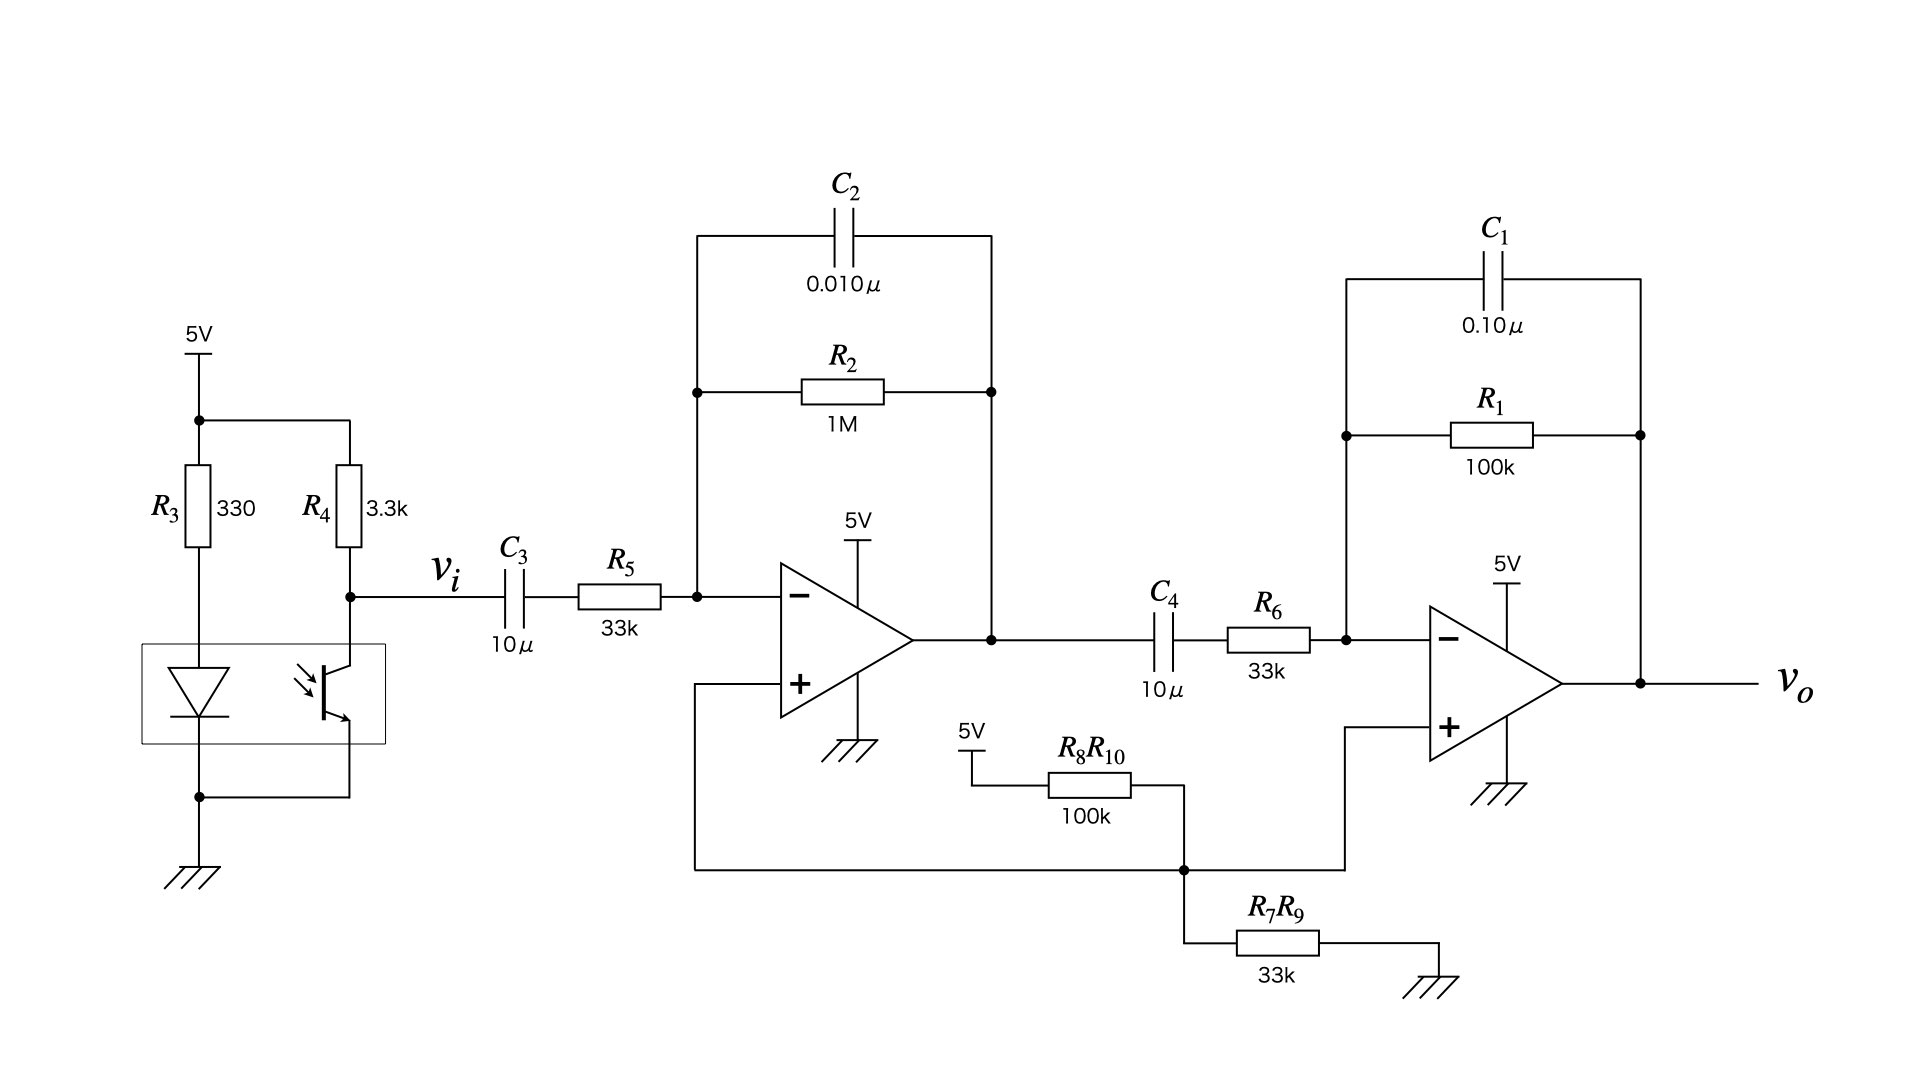
\includegraphics[width=1\linewidth]{fig_work_A/2_fig.jpg}
  \caption{ワークA-2 回路図}
  \label{fig:2_fig}
\end{figure}

\subsection{ワークA-1: センサ後段回路}
設計した増幅・フィルタ回路の特性を評価するため，図\ref{fig:1_fig}に示す回路を図\ref{fig:1_pic}のように実装した．
入力端子には，波形出力デバイス(ATOM Lite)を1M$\Omega$の抵抗($R_{11}$)を介して接続した．
\begin{figure}[H]
  \centering
  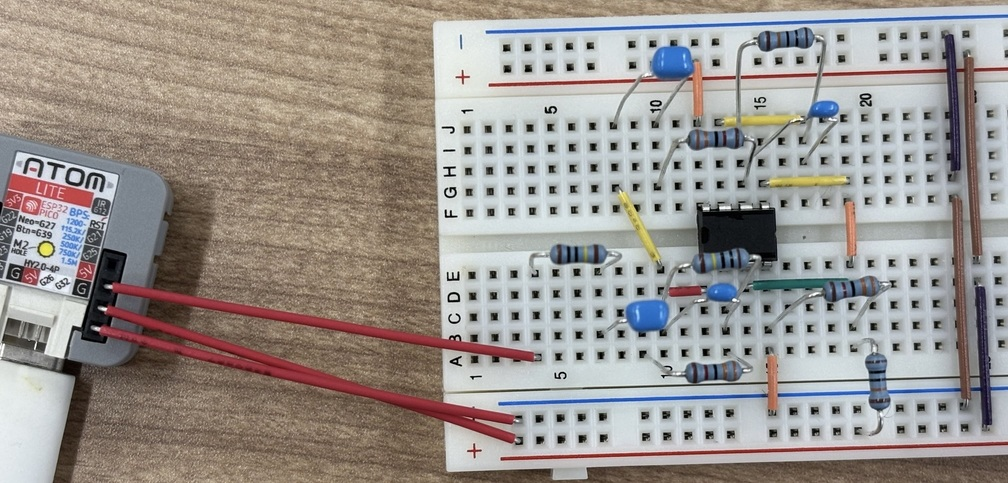
\includegraphics[width=0.9\linewidth]{fig_work_A/1_pic.jpg}
  \caption{ワークA-1 実装回路}
  \label{fig:1_pic}
\end{figure}

まず，回路の各増幅段が設計通りに動作することを確認するため，1Hzの正弦波を入力し，以下の3点についてオシロスコープで観測を行う．
\begin{enumerate}
  \item 一段目(-30.3倍)の動作確認: 回路の入力($v_1$)と一段目の出力($v_2$)を観測し，増幅率と位相の反転を確認する．
  \item 二段目(-3.03倍)の動作確認: 一段目の出力($v_2$)と回路全体の出力($v_o$)を観測し，増幅率と位相の反転を確認する．
  \item 増幅回路全体(91.8倍)の動作確認: 回路の入力($v_1$)と出力($v_o$)を観測し，全体の増幅率を確認する．
\end{enumerate}

次に，4種類の波形(1Hz正弦波，1Hzと100Hzの合成波，1Hzと7Hzの合成波，脈波)をそれぞれ入力し，入力($v_1$)と出力($v_o$)をオシロスコープで観測する．
観測では，各波形の周期，振幅，および入出力間の時間差を測定する．

\newpage

\subsection{ワークA-2: 脈拍検出回路}
ワークA-1の回路の入力部を，設計した脈拍検出回路に置き換え，図\ref{fig:2_fig}に示す回路を図\ref{fig:2_pic}のように実装した．
\begin{figure}[H]
  \centering
  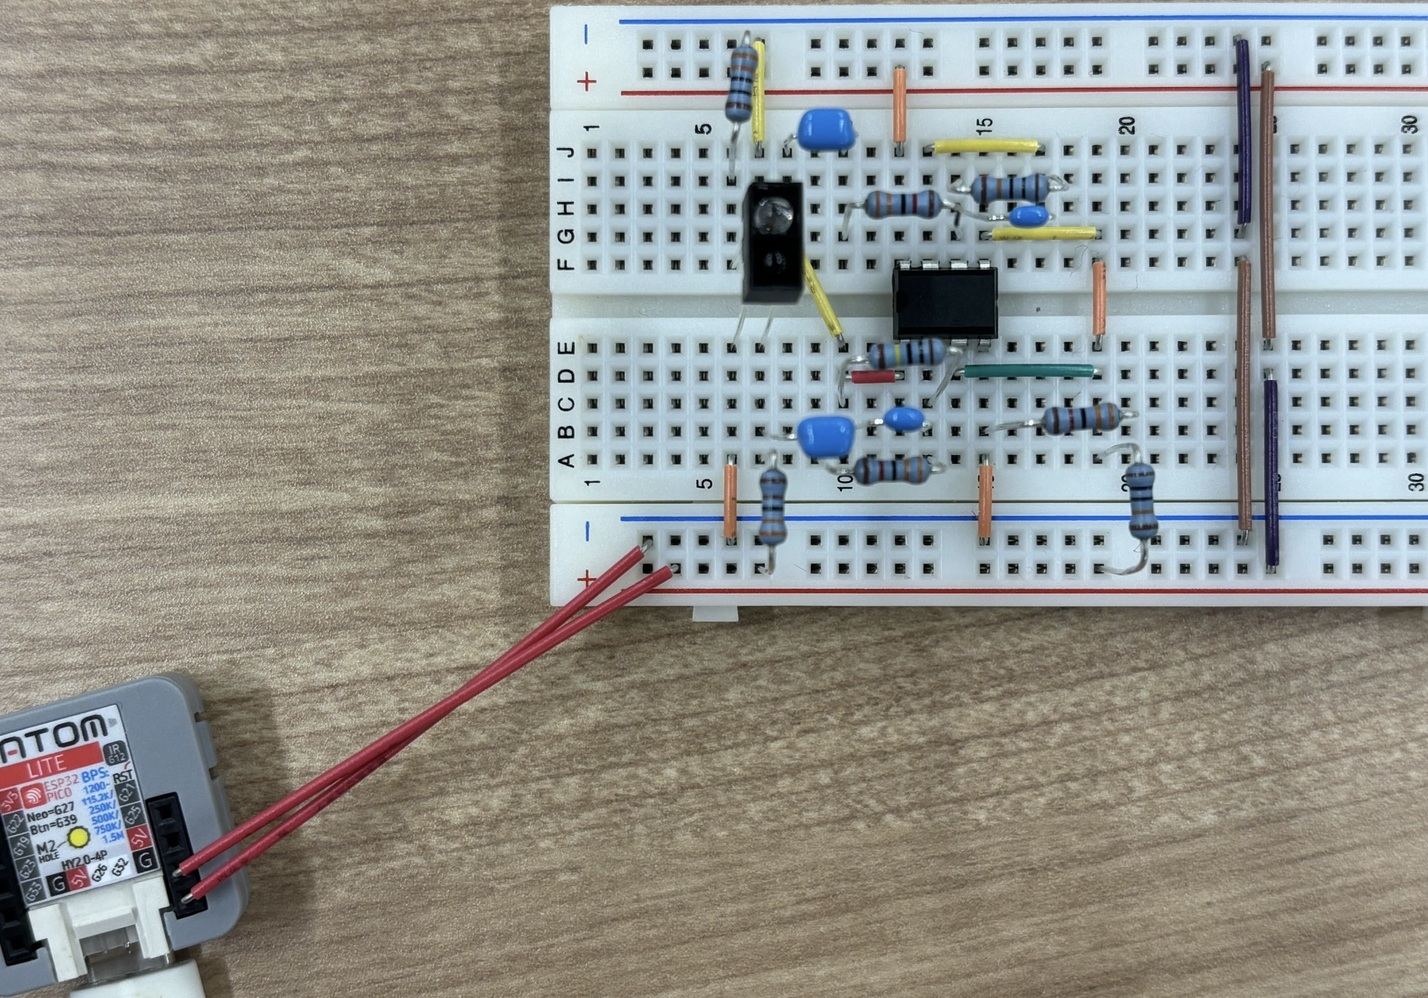
\includegraphics[width=0.9\linewidth]{fig_work_A/2_pic.jpg}
  \caption{ワークA-2 実装回路}
  \label{fig:2_pic}
\end{figure}
フォトリフレクタに指を置き，オシロスコープで脈波検出回路から出力された脈波($v_i$)と最終的な脈波($v_o$)を観測する．
この際，出力電圧の振幅が仕様(1V以上，4V未満)を満たすことを確認する．


\newpage

\section{結果} 
%% 実験から得られた結果を，目的や方法を理解した上で，重要データを外す
%% ことなく，要領よくまとめてください．
%% 
%% 結果（数値）は，（自分はポイントを理解しているということをアピール
%% しながら）視認性（一覧性）を高めて報告することが求められる．この意
%% 味で，要領よくまとめられた表が望ましい．決して，文章の中にバラバラ
%% に埋没させて，読み手がどこに書いているか分かりにくい（書き手にとっ
%% ては都合のよい）記載するものではない点に注意する．
%% 
%% 
%% 結果をまとめた表の例
%% ただし，ワーク前の説明で話した通り，
%%   - 一次データ（生データ）
%%   - 計器パラメータ（レンジなど）
%%   - 中間算出値（二次以上の高次データ）
%%   - 周期，時間差，入力電位，出力電位（必須データ）
%%   - 手順書の課題4.で求められるデータ（必須データ）
%% を記録した表に書き換えて，結果報告してください．

\subsection{ワークA-1: センサ後段回路}
\subsubsection{各増幅段の動作確認}
回路の各増幅段が設計通りに動作することを確認するため，1Hzの正弦波を入力し，各段の入出力波形を観測した．
一段目(-30.3倍)および二段目(-3.03倍)，並びに一段目と二段目を合わせた回路全体のオシロスコープ画面を，
それぞれ図\ref{fig:1_green_v1v2}，図\ref{fig:1_green_v2vo}，図\ref{fig:1_green_v1vo}に示す．
\begin{figure}[H]
  \centering
  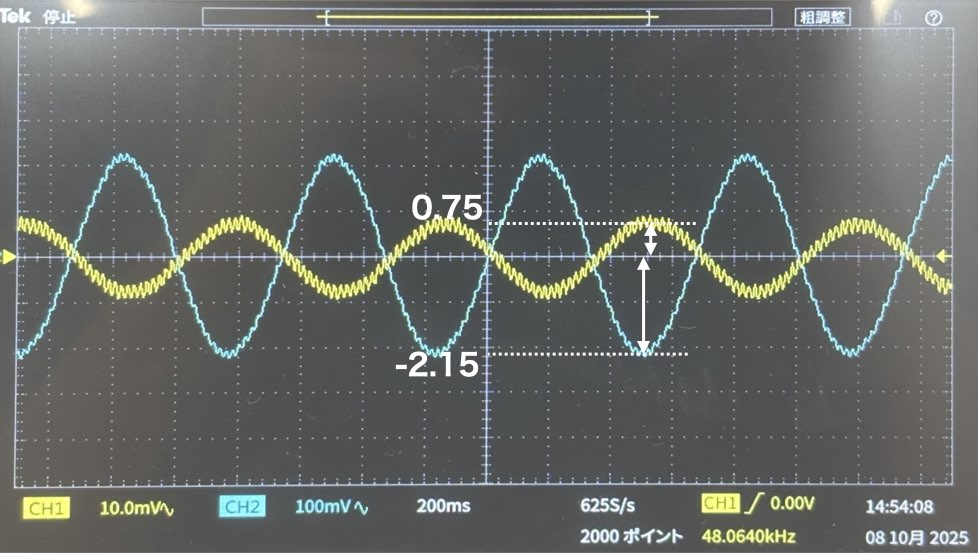
\includegraphics[width=0.8\linewidth]{fig_work_A/1_green_v1v2.jpg}
  \caption{一段目増幅回路の入出力波形(黄:$v_1$，青:$v_2$)．図中の書き込みは，表\ref{tab:result1-1}の一段目の目盛り読み取り値を示す．}
  \label{fig:1_green_v1v2}
\end{figure}
\begin{figure}[H]
  \centering
  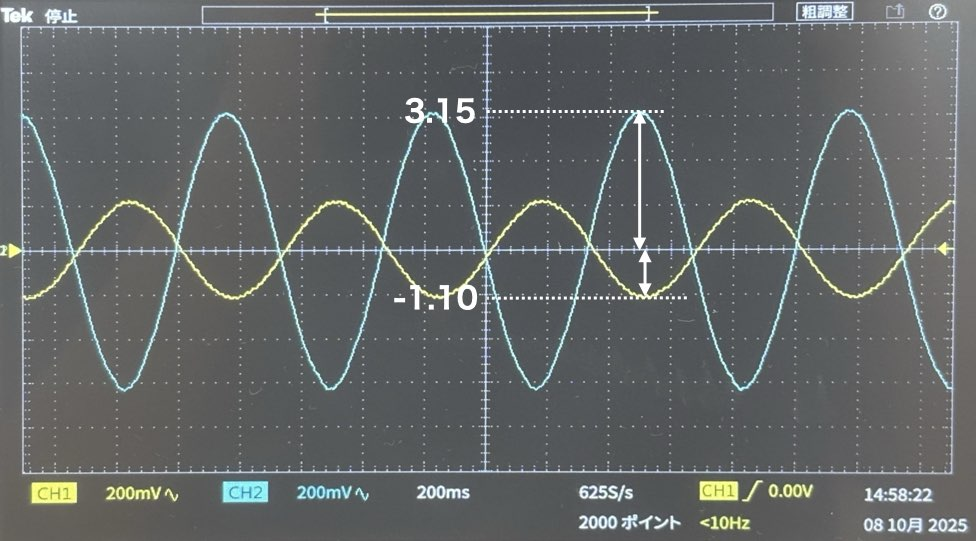
\includegraphics[width=0.8\linewidth]{fig_work_A/1_green_v2vo.jpg}
  \caption{二段目増幅回路の入出力波形(黄:$v_2$，青:$v_o$)．図中の書き込みは，表\ref{tab:result1-1}の二段目の目盛り読み取り値を示す．}
  \label{fig:1_green_v2vo}
\end{figure}
\begin{figure}[H]
  \centering
  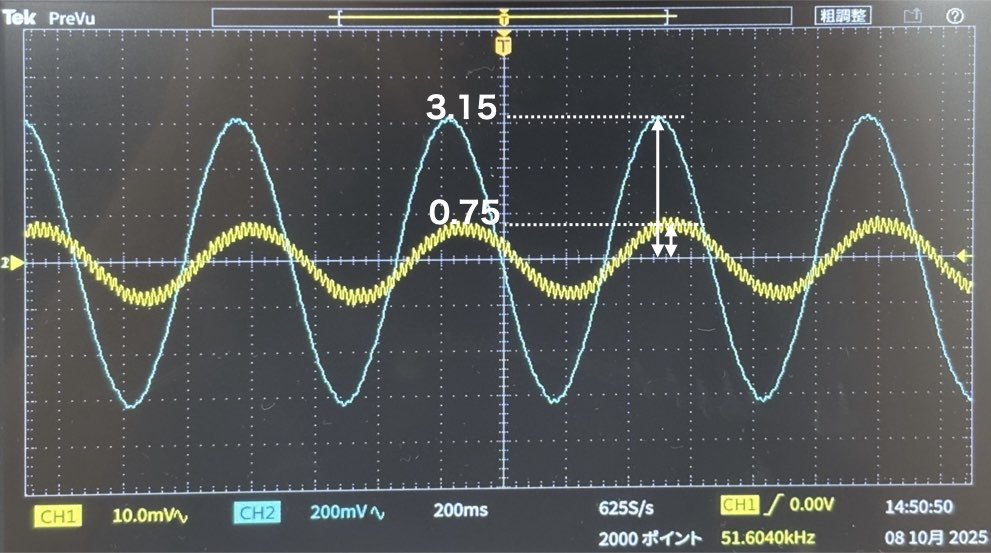
\includegraphics[width=0.8\linewidth]{fig_work_A/1_green_v1vo.jpg}
  \caption{二段反転増幅回路の入出力波形(黄:$v_1$，青:$v_o$)．図中の書き込みは，表\ref{tab:result1-1}の回路全体の目盛り読み取り値を示す．}
  \label{fig:1_green_v1vo}
\end{figure}
測定値から算出した各段の増幅率を表\ref{tab:result1-1}にまとめる．
\begin{table}[H]
  \caption{各増幅段の増幅率}
  \centering
  \begin{tabular}{|c|c|c|c|c|c|c|}
    \hline
    \multirow{2}{*}{増幅段} & \multirow{2}{*}{信号} & スケール & 読み取り値 & 測定電圧 & 測定増幅率 & 設計増幅率 \\
     & & [V/div] & [div] & [mV] & [倍] & [倍] \\
    \hline \hline
    \multirow{2}{*}{一段目} & 入力($v_1$) & 10.0m & 0.75 & 7.50 & \multirow{2}{*}{-28.6} & \multirow{2}{*}{-30.3} \\
    \cline{2-5}
     & 出力($v_2$) & 100m & -2.15 & -215 & & \\
    \hline
    \multirow{2}{*}{二段目} & 入力($v_2$) & 200m & -1.10 & -220 & \multirow{2}{*}{-2.86} & \multirow{2}{*}{-3.03} \\
    \cline{2-5}
     & 出力($v_o$) & 200m & 3.15 & 630 & & \\
    \hline
    \multirow{2}{*}{回路全体} & 入力($v_1$) & 10.0m & 0.75 & 7.50 & \multirow{2}{*}{84.0} & \multirow{2}{*}{91.8} \\
    \cline{2-5}
     & 出力($v_o$) & 200m & 3.15 & 630 & & \\
    \hline
  \end{tabular}
  \label{tab:result1-1}
\end{table}

\newpage


\subsubsection{回路全体の周波数特性評価}
回路全体の特性を評価するため，4種類の波形を入力した際のオシロスコープ画面を図\ref{fig:1_green}，図\ref{fig:1_red}，図\ref{fig:1_red2}，
図\ref{fig:1_blue}，図\ref{fig:1_blue2}，図\ref{fig:1_purple}，図\ref{fig:1_purple2}に示す．
\begin{figure}[H]
  \centering
  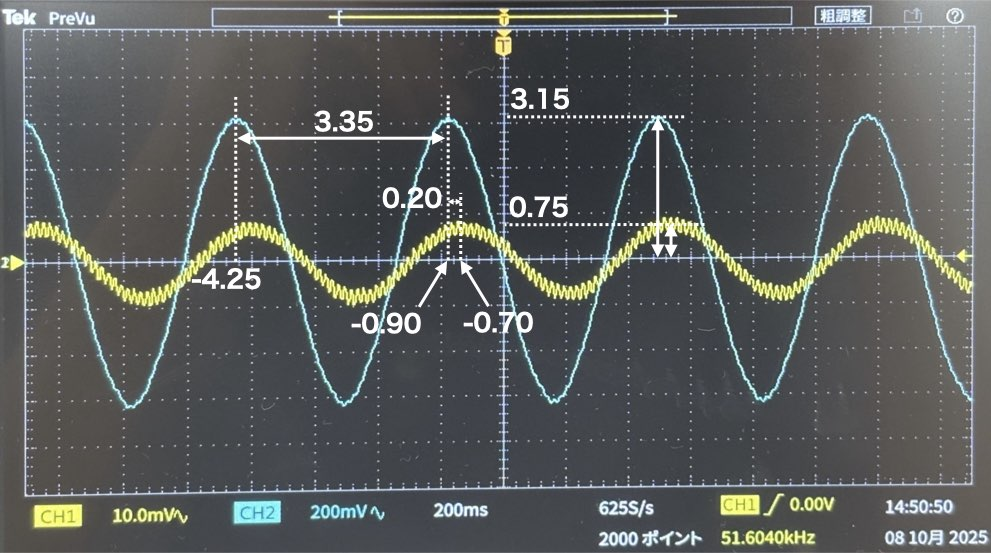
\includegraphics[width=0.9\linewidth]{fig_work_A/1_green.jpg}
  \caption{1Hz正弦波(黄:$v_1$，青:$v_o$)．図中の書き込みは，表\ref{tab:result1-2}の波形1の目盛り読み取り値を示す．}
  \label{fig:1_green}
\end{figure}
\begin{figure}[H]
  \centering
  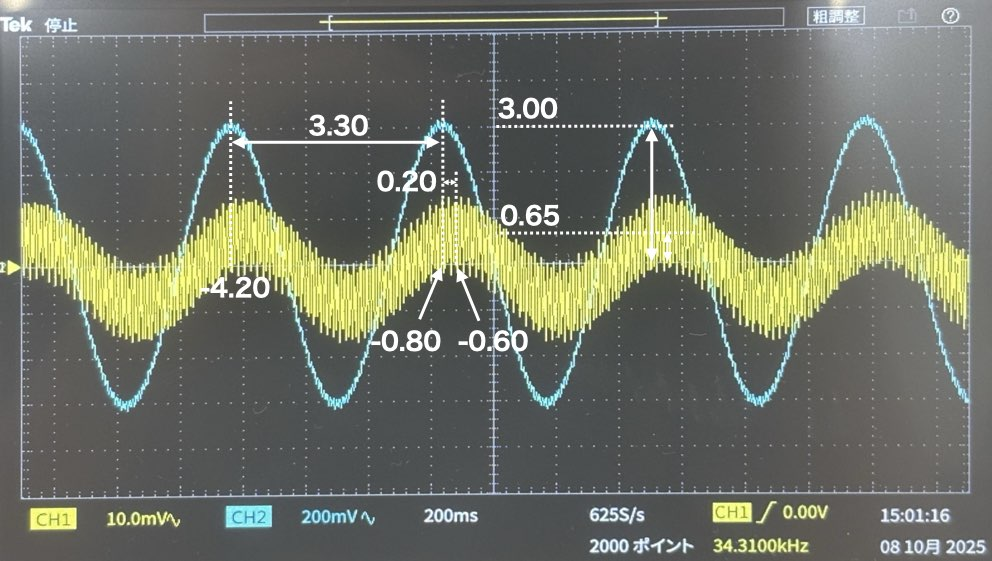
\includegraphics[width=0.9\linewidth]{fig_work_A/1_red.jpg}
  \caption{1Hzと100Hzの合成波(黄:$v_1$，青:$v_o$)．図中の書き込みは，表\ref{tab:result1-2}の波形2，低周波成分の目盛り読み取り値を示す．}
  \label{fig:1_red}
\end{figure}
\begin{figure}[H]
  \centering
  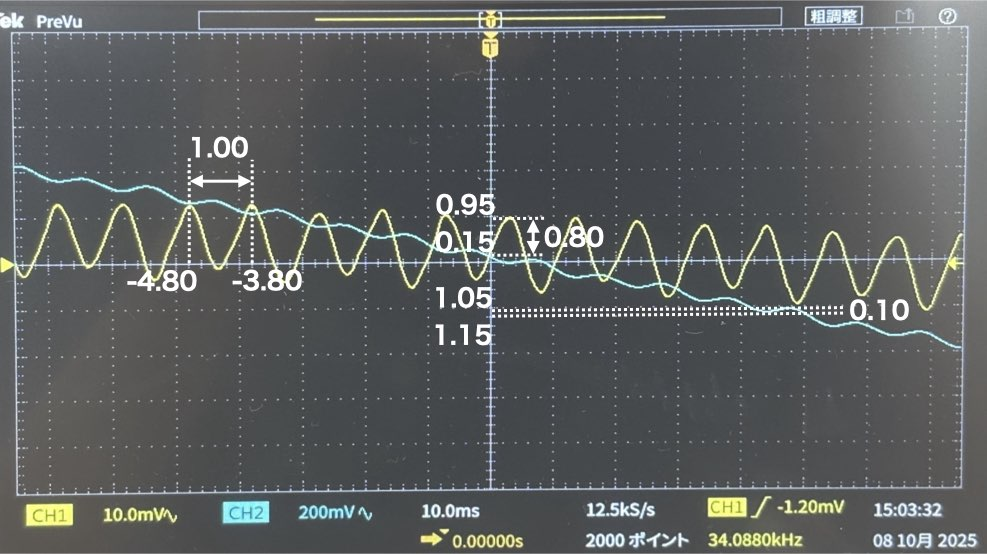
\includegraphics[width=0.9\linewidth]{fig_work_A/1_red2.jpg}
  \caption{時間軸を拡大した1Hzと100Hzの合成波(黄:$v_1$，青:$v_o$)．図中の書き込みは，表\ref{tab:result1-2}の波形2，高周波成分の目盛り読み取り値を示す．}
  \label{fig:1_red2}
\end{figure}
\begin{figure}[H]
  \centering
  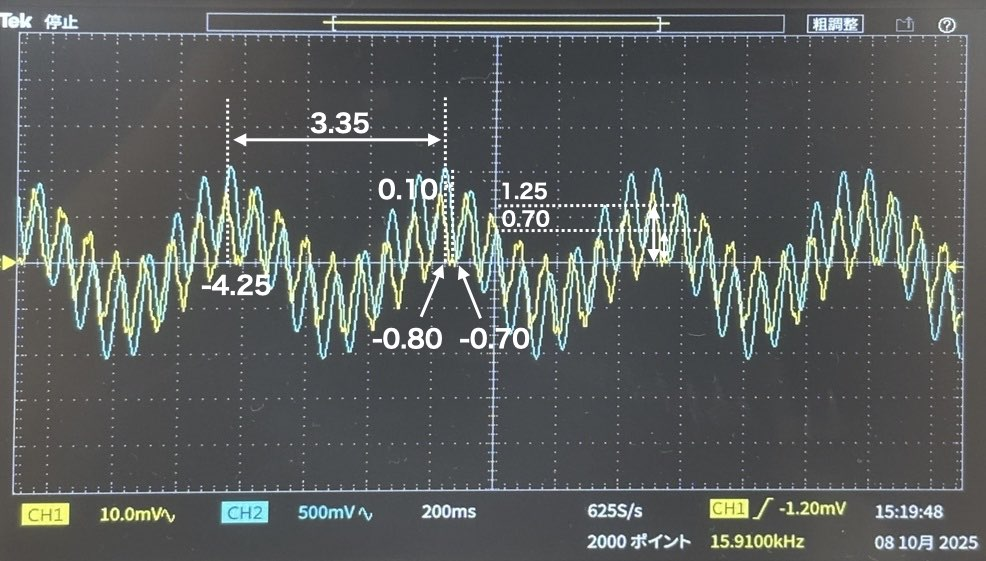
\includegraphics[width=0.9\linewidth]{fig_work_A/1_blue.jpg}
  \caption{1Hzと7Hzの合成波(黄:$v_1$，青:$v_o$)．図中の書き込みは，表\ref{tab:result1-2}の波形3，低周波成分の目盛り読み取り値を示す．}
  \label{fig:1_blue}
\end{figure}
\begin{figure}[H]
  \centering
  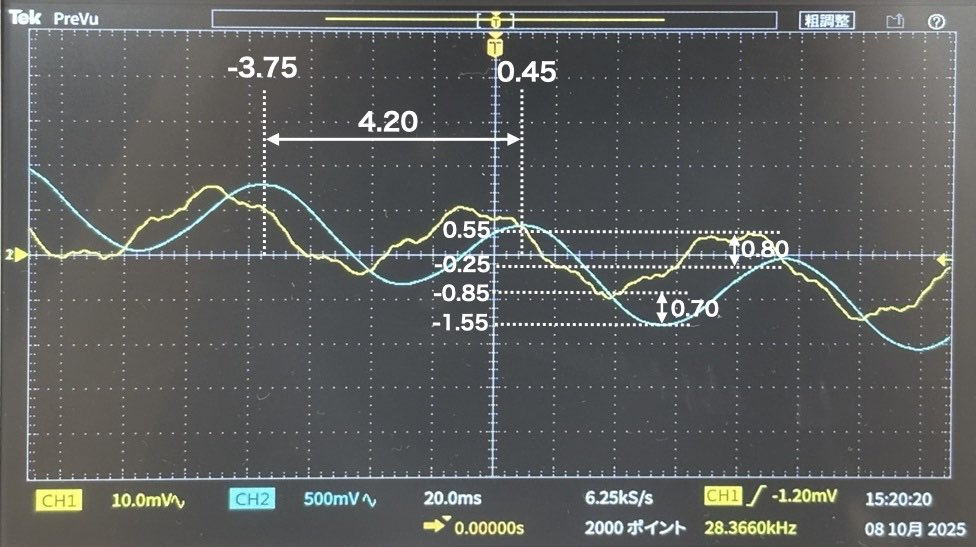
\includegraphics[width=0.9\linewidth]{fig_work_A/1_blue2.jpg}
  \caption{時間軸を拡大した1Hzと7Hzの合成波(黄:$v_1$，青:$v_o$)．図中の書き込みは，表\ref{tab:result1-2}の波形3，高周波成分の目盛り読み取り値を示す．}
  \label{fig:1_blue2}
\end{figure}
\begin{figure}[H]
  \centering
  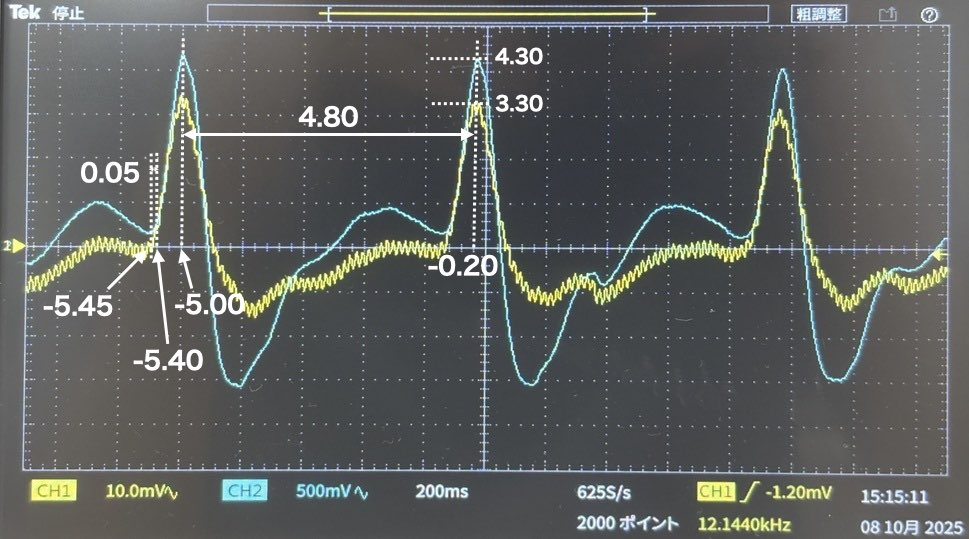
\includegraphics[width=0.9\linewidth]{fig_work_A/1_purple.jpg}
  \caption{脈波(黄:$v_1$，青:$v_o$)．図中の書き込みは，表\ref{tab:result1-2}の波形4，低周波成分の目盛り読み取り値を示す．}
  \label{fig:1_purple}
\end{figure}
\begin{figure}[H]
  \centering
  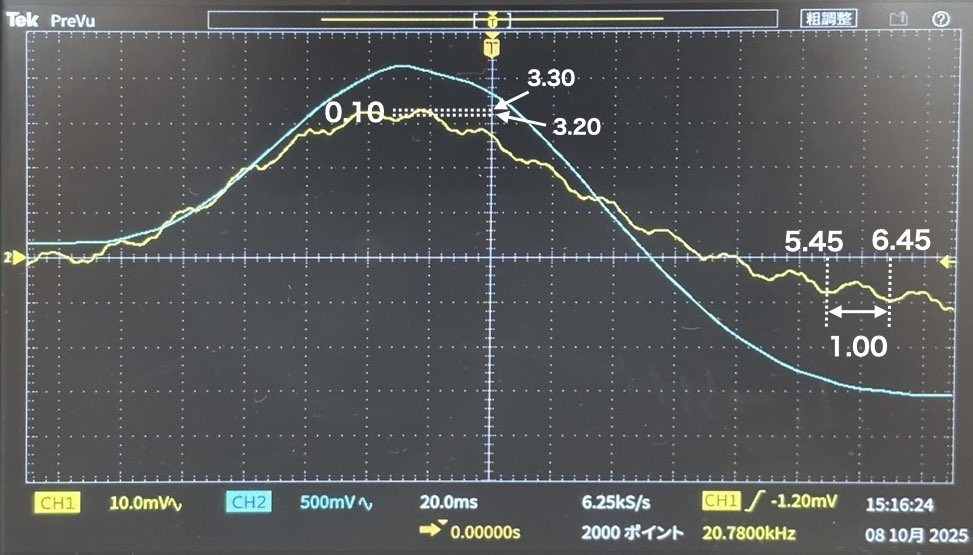
\includegraphics[width=0.9\linewidth]{fig_work_A/1_purple2.jpg}
  \caption{時間軸を拡大した脈波(黄:$v_1$，青:$v_o$)．図中の書き込みは，表\ref{tab:result1-2}の波形4，高周波成分の目盛り読み取り値を示す．}
  \label{fig:1_purple2}
\end{figure}
各波形を観測した際の計測結果を表\ref{tab:result1-2}にまとめ，
表\ref{tab:result1-2}の計測結果から算出した数値を表\ref{tab:result1-3}にまとめる．
\begin{table}[H]
  \caption{波形出力デバイスの計測における読み取り値(一次データ)}
  \centering
  \begin{tabular}{|c|c|c|c|c|c|c|c|}
    \hline
    \multirow{2}{*}{波形} & \multirow{2}{*}{成分} & \multirow{2}{*}{信号} & スケール & 読み取り値 & \multirow{2}{*}{項目} & スケール & 読み取り値 \\[-4pt]
    & & & [mV/div] & [div] & & [ms/div] & [div] \\
    \hline \hline
    \multirow{2}{*}{1} & \multirow{2}{*}{低周波} & 入力 ($v_1$) & 10.0 & 0.75 & 周期 & 200 & 3.35 \\
    \cline{3-8}
    & & 出力 ($v_o$) & 200 & 3.15 & 時間差 & 200 & 0.20 \\
    \hline
    \multirow{4}{*}{2} & \multirow{2}{*}{低周波} & 入力 ($v_1$) & 10.0 & 0.65 & 周期 & 200 & 3.30 \\
    \cline{3-8}
    & & 出力 ($v_o$) & 200 & 3.00 & 時間差 & 200 & 0.20 \\
    \cline{2-8}
    & \multirow{2}{*}{高周波} & 入力 ($v_1$) & 10.0 & 0.80 & \multirow{2}{*}{周期} & \multirow{2}{*}{10.0} & \multirow{2}{*}{1.00} \\
    \cline{3-5}
    & & 出力 ($v_o$) & 200 & 0.10 & & & \\
    \hline
    \multirow{4}{*}{3} & \multirow{2}{*}{低周波} & 入力 ($v_1$) & 10.0 & 0.70 & 周期 & 200 & 3.35 \\
    \cline{3-8}
    & & 出力 ($v_o$) & 500 & 1.25 & 時間差 & 200 & 0.10 \\
    \cline{2-8}
    & \multirow{2}{*}{高周波} & 入力 ($v_1$) & 10.0 & 0.80 & \multirow{2}{*}{周期} & \multirow{2}{*}{20.0} & \multirow{2}{*}{4.20} \\
    \cline{3-5}
    & & 出力 ($v_o$) & 500 & 0.70 & & & \\
    \hline
    \multirow{4}{*}{4} & \multirow{2}{*}{低周波} & 入力 ($v_1$) & 10.0 & 3.30 & 周期 & 200 & 4.80 \\
    \cline{3-8}
    & & 出力 ($v_o$) & 500 & 4.30 & 時間差 & 200 & 0.05 \\
    \cline{2-8}
    & \multirow{2}{*}{高周波} & 入力 ($v_1$) & 10.0 & 0.10 & \multirow{2}{*}{周期} & \multirow{2}{*}{20.0} & \multirow{2}{*}{1.00} \\
    \cline{3-5}
    & & 出力 ($v_o$) & 500 & (測定不能) & & & \\
    \hline
  \end{tabular}
  \label{tab:result1-2}
\end{table}
\begin{table}[H]
  \caption{一次データに基づく算出結果(高次データ)}
  \centering
  \small
  \begin{tabular}{|c|c|c|c|c|c|c|c|c|c|}
    \hline
    \multirow{2}{*}{波形} & \multirow{2}{*}{成分} & 時間差 & ~周期~ & 測定周波数 & 設計周波数 & $v_1$振幅 & $v_o$振幅 & 増幅率 & 脈拍数 \\[-4pt]
    & & [ms] & [ms] & [Hz] & [Hz] & [mV] & [mV] & [倍] & [bpm] \\
    \hline \hline
    1 & 低周波 & 40.0 & 670 & 1.49 & 1 & 7.50 & 630 & 84.0 & - \\
    \hline
    \multirow{2}{*}{2} & 低周波 & 40.0 & 660 & 1.51 & 1 & 6.50 & 600 & 92.3 & - \\
    \cline{2-10}
    & 高周波 & - & 10.0 & 100 & 100 & 8.00 & 20.0 & 2.50 & - \\
    \hline
    \multirow{2}{*}{3} & 低周波 & 20.0 & 670 & 1.49 & 1 & 7.00 & 625 & 89.3 & - \\
    \cline{2-10}
    & 高周波 & - & 84.0 & 11.9 & 7 & 8.00 & 350 & 43.8 & - \\
    \hline
    \multirow{2}{*}{4} & 低周波 & 10.0 & 960 & 1.04 & - & 33.0 & $2.15 \times 10^3$ & 65.2 & 62.5 \\
    \cline{2-10}
    & 高周波 & - & 20.0 & 50.0 & - & 1.00 & (測定不能) & (測定不能) & - \\
    \hline
  \end{tabular}
  \label{tab:result1-3}
\end{table}


\subsection{ワークA-2: 脈拍検出回路の評価}
最終的に，フォトリフレクタに指を置き，脈拍を測定した．
オシロスコープで観測した脈波の波形を図\ref{fig:2_result}に示す．
\begin{figure}[H]
  \centering
  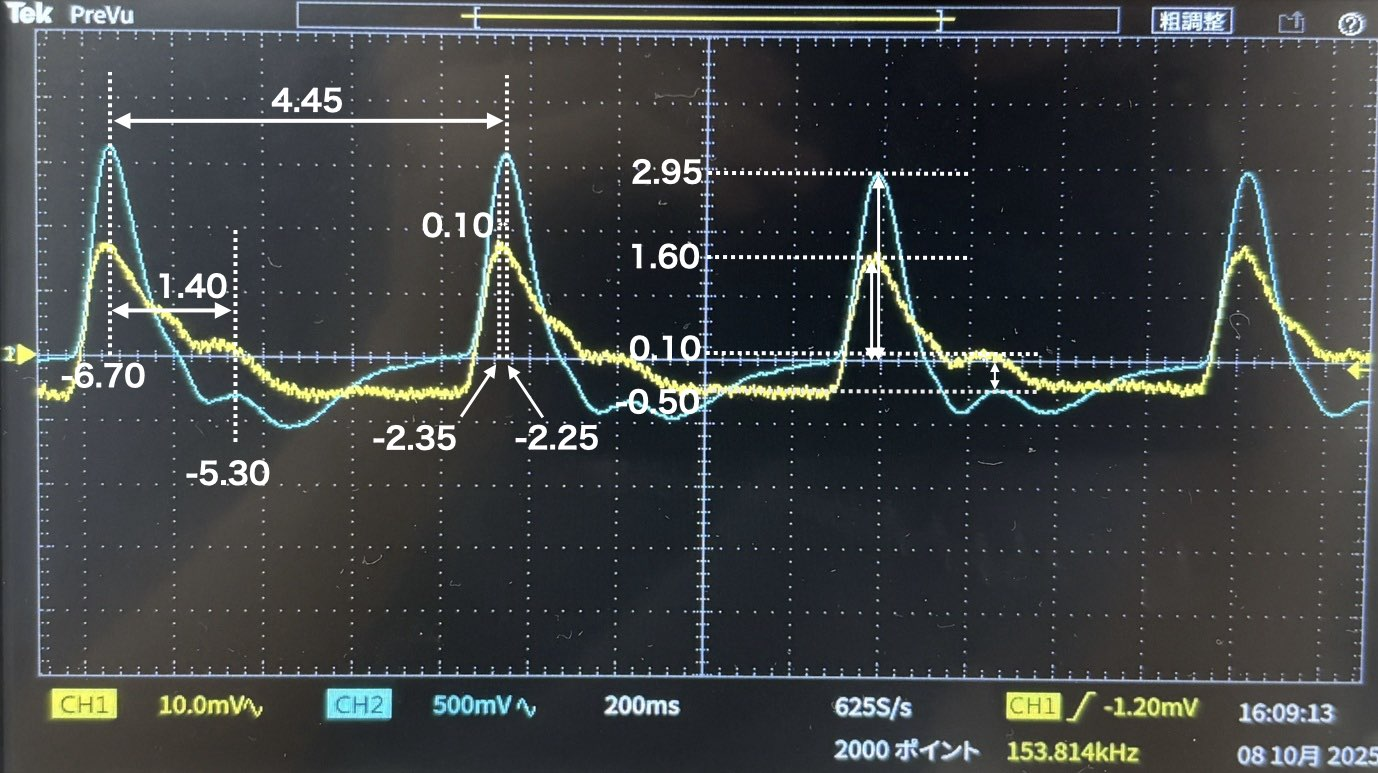
\includegraphics[width=0.9\linewidth]{fig_work_A/2_result.jpg}
  \caption{測定した自身の脈波(黄:$v_i$，青:$v_o$)．図中の書き込みは，表\ref{tab:result2-1}の主脈波および副脈波の目盛り読み取り値を示す．}
  \label{fig:2_result}
\end{figure}
\newpage
また，観測された波形の計測結果を表\ref{tab:result2-1}にまとめ，
表\ref{tab:result2-1}の計測結果から算出した数値を表\ref{tab:result2-2}にまとめる．
\begin{table}[H]
  \caption{脈拍測定における読み取り値(一次データ)}
  \centering
  \begin{tabular}{|c|c|c|c|}
    \hline
    \multirow{2}{*}{測定項目} & \multirow{2}{*}{信号} & \multicolumn{2}{c|}{電圧測定} \\
    \cline{3-4}
    & & スケール [mV/div] & 読み取り値 [div] \\
    \hline
    \multirow{2}{*}{主脈波} & 入力($v_i$) & 10.0 & 1.60 \\
    \cline{2-4}
     & 出力($v_o$) & 500 & 2.95 \\
    \hline
    \multirow{2}{*}{副脈波} & 入力($v_i$) & 10.0 & 0.10 \\
    \cline{2-4}
     & 出力($v_o$) & 500 & -0.50 \\
    \hline \hline
    \multirow{2}{*}{測定項目} & \multirow{2}{*}{項目} & \multicolumn{2}{c|}{時間測定} \\
    \cline{3-4}
     & & スケール [ms/div] & 読み取り値 [div] \\
    \hline
    主脈波 & 周期 & 200 & 4.45 \\
    \cline{2-4}
    と & 時間差 & 200 & 0.10 \\
    \cline{2-4}
    副脈波 & 間隔 & 200 & 1.40 \\
    \hline
  \end{tabular}
  \label{tab:result2-1}
\end{table}
\begin{table}[H]
  \caption{一次データに基づく算出結果(高次データ)}
  \centering
  \begin{tabular}{|c|c|c|c|c|c|c|c|c|}
    \hline
    \multirow{2}{*}{信号} & $v_i$振幅 & $v_o$振幅 & 増幅率 & 時間差 & 周期 & 周波数 & 脈拍数 & ~間隔~ \\[-4pt]
     & {[mV]} & {[mV]} & {[倍]} & {[ms]} & {[ms]} & {[Hz]} & {[bpm]} & {[ms]} \\
    \hline \hline
    主脈波 & 16.0 & 1475 & 92.2 & \multirow{2}{*}{20.0} & \multirow{2}{*}{890} & \multirow{2}{*}{1.12} & \multirow{2}{*}{67.4} & \multirow{2}{*}{280} \\
    \cline{1-4}
    副脈波 & 1.00 & -250 & -250 & & & & & \\
    \hline
  \end{tabular}
  \label{tab:result2-2}
\end{table}
\newpage
さらに，フォトリフレクタに指を置いた直後の波形を図\ref{fig:2_result2}に示し，図\ref{fig:2_result2}で観測された出力($v_o$)の遅延時間を表\ref{tab:result2-3}にまとめる．
\begin{figure}[H]
  \centering
  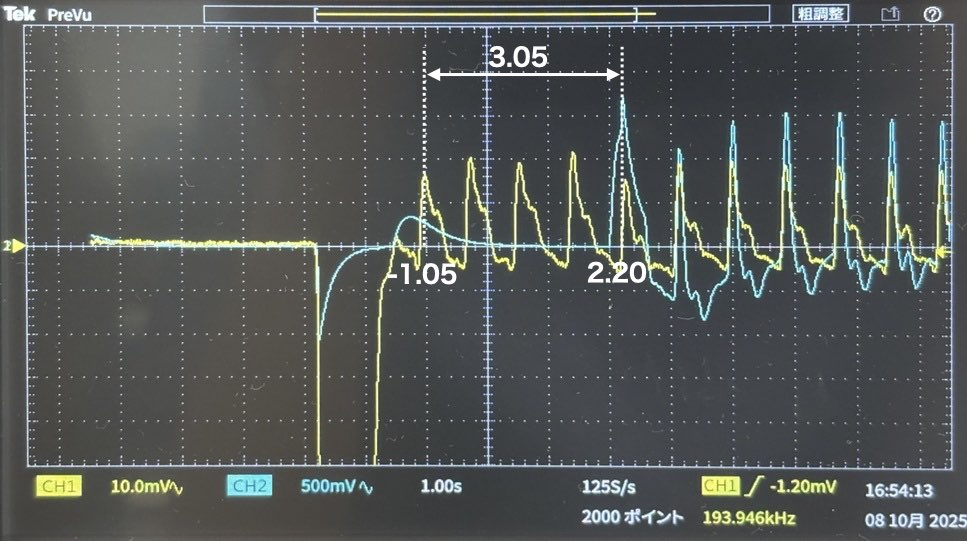
\includegraphics[width=0.9\linewidth]{fig_work_A/2_result2.jpg}
  \caption{フォトリフレクタに指を置いた直後の波形(黄:$v_i$，青:$v_o$)．図中の書き込みは，表\ref{tab:result2-3}の入力($v_i$)で波形が現れてから出力($v_o$)で波形が現れるまでの遅延時間の目盛り読み取り値を示す．}
  \label{fig:2_result2}
\end{figure}
\begin{table}[H]
  \caption{入力($v_i$)で波形が現れてから出力($v_o$)で波形が現れるまでの遅延時間}
  \centering
  \begin{tabular}{|c|c|c|}
    \hline
    スケール [s/div] & 読み取り値 [div] & 遅延時間[s] \\
    \hline \hline
    1.00 & 3.05 & 3.05 \\
    \hline
  \end{tabular}
  \label{tab:result2-3}
\end{table}


%% 必ず下記のものは写真を撮るなどして図として報告書に記載してください．
%% 実装した回路
%% オシロスコープに表示された自分の脈波

%\begin{figure}[ht]
%\begin{center}
%\includegraphics[width=0.95\textwidth,clip]{fig_work_A/}
%\end{center}
%\caption{\textgt{
%    図の内容を表す適切なキャプションをつける
%}}
%\label{sample}
%\end{figure}



\section{考察}
%% 手順書の「４ 考察」であげた３項目を含み，結果（数値）に対する自分の
%% 考えを述べよ．
%% 感想とならないよう，数値に基づいた定量的な考察となるように注意する．


\subsection{増幅率と周波数特性}
設計した回路の増幅およびフィルタ性能について，測定結果から考察する．
まず，誤差の主な原因として，使用した抵抗器(許容差±5\%)およびコンデンサ(許容差±10\%)の部品個体差が複合的に作用したことが考えられる．

次に，回路の各増幅段の動作を確認した．
表\ref{tab:result1-1}より，一段目の測定増幅率は-28.6倍(設計値-30.3倍)，二段目は-2.86倍(設計値-3.03倍)となり，
各段において設計値に非常に近い増幅率が得られた．これは，各増幅段が個別にほぼ設計通りに動作していることを示している．
また，増幅回路全体の測定増幅率は84.0倍(設計値91.8倍)となり，設計値より約-8.5\%の誤差が生じたものの，
部品の個体差を考慮すれば，回路全体としてもほぼ設計通りに機能していることを示している．

続いて，回路全体の周波数特性を，各周波数における増幅率から評価する．
表\ref{tab:result1-3}より，通過可能な周波数の範囲内にある1.49Hzや1.51Hzの信号に対する増幅率は，波形1で84.0倍，波形2で92.3倍，波形3で89.3倍であり，設計増幅率91.8倍に近い値を示した．
したがって，回路が通過帯域内の信号を意図通りに増幅していることが確認できた．

さらに，高周波数成分に対する増幅率を評価する．
表\ref{tab:result1-3}より，上限周波数16Hzに近い11.9Hz成分(波形3)では，増幅率が43.8倍に低下していた．
この結果は偶然誤差の影響も考えられるが，フィルタの減衰効果が上限周波数で急に始まるのではなく，
通過可能な周波数の範囲内であっても，上限周波数に近づくにつれて増幅率が低下し始めることも考えられる．
また，上限周波数を大幅に超える100Hz成分(波形2)では，増幅率がわずか2.50倍にまで低下し，50.0Hz(波形4)に至っては，出力側($v_o$)で観測が不可能なレベルになっていた．
この結果は，設計した回路が高周波ノイズを効果的に減衰させる能力を持つことを示している．

以上の結果から，測定された増幅率は周波数によって変動するものの，それは設計したバンドパスフィルタの特性を反映したものであり，
部品の許容差を考慮すれば，本回路はほぼ設計通りの増幅およびフィルタ性能を持つと結論付けられる．



\subsection{脈拍検出回路}
まず，表\ref{tab:result2-2}より，測定した脈拍数は67.4bpmであり，一般的な安静時の脈拍数として妥当な値である\cite{workA_脈拍数}．
このとき，回路全体の増幅率は92.2倍となり，設計値91.8倍とほぼ一致した．
したがって，ワークA-1で性能を評価した回路が，実際の微弱な生体信号(脈波)に対しても有効に機能し，
観測に適したレベルまで増幅できることが実証された．

次に，観測された図\ref{fig:2_result}の脈波の波形には，最も振幅の大きな主脈波の280ms後に，振幅の小さな副脈波が確認できる．
表\ref{tab:result2-2}からも，これは単なるノイズとは異なる周期的な特徴であることがわかる．
本回路が，主となる脈の周期成分だけでなく，それに重複したこのような微細な電圧変動までも増幅できていることは，
設計したフィルタ増幅回路が十分な感度と性能を有していることを示している．

一方で，表\ref{tab:result2-2}において，副脈波の増幅率は-250倍となった．
回路の設計増幅率は正の値(+91.8倍)であり，主脈派はそれに沿った正常な増幅率(+92.2倍)であることから，この測定結果は矛盾している．
この原因として，測定時の基準電圧の設定に問題があった可能性が考えられる．
オシロスコープの時間軸（中央線）を0V基準として読み取りを行ったが，実際の信号のグラウンドがこの基準線と正確に一致していなかった可能性がある．
そのため，本来は$v_o$と同様に基準線より下に振れていたはずの$v_i$の副脈波が，基準レベルのずれにより，見かけ上プラスの値として読み取られてしまい，
回路の増幅特性とは矛盾した測定結果になったと考察される．

\newpage

さらに，図\ref{fig:2_result2}では，フォトリフレクタに指を置いた直後の応答が観測されている．
入力側($v_i$)では脈波がすぐに検出されているにもかかわらず，出力側($v_o$)で初めて検出されたのは，表\ref{tab:result2-3}より，入力側($v_i$)で検出された3.05秒後であった．
これには，コンデンサが関係していると考えられる．
指を置いた瞬間にセンサの電圧レベルが大きく変化するため，コンデンサが変化後の電圧に合わせて充電されるまでに一定の時間が必要となる．
これが完了するまでの間は，後段の増幅回路が正しく動作できず，入力された脈波信号が出力されなかったと考察される．



\subsection{入出力間の時間差}
表\ref{tab:result1-3}および表\ref{tab:result2-2}に示すように，全ての波形において入力($v_1$)と出力($v_o$)の間に数十msの時間差が観測された．
これは，回路に含まれるコンデンサと抵抗によって構成されるフィルタ回路に起因する位相差である．
ハイパスフィルタとして機能する入力段の回路は位相を進ませ，ローパスフィルタとして機能する帰還部の回路は位相を遅らせる特性を持つ．
観測された時間差は，これら二段のフィルタ回路による位相変化が時間として現れたものであると考えられる．





\section{おわりに} 
%% ワークAを通じて得られた知見や考察，目的の達成度などについて記述し，ワー
%% クAを総括する．単なる感想ではなく，客観的な総括を行うように注意する．
本実習では，フォトリフレクタとオペアンプを用いて，脈拍を検出するためのフィルタ増幅回路の設計と実装を行った．
はじめに，バンドパスフィルタ付き二段反転増幅回路を設計し，その特性評価を行った．
結果として，回路は設計通りの増幅率と周波数特性を持つことが確認できた．
次に，この回路とフォトリフレクタを用いたセンサ部を組み合わせ，自身の脈波を測定した．
その結果，67.4bpmという妥当な脈拍数を観測でき，回路が実際の生体信号に対しても有効に機能することが実証された．
また，脈波に含まれる微細な特徴や，指を置いた直後にコンデンサが充電されることで生じる出力遅延といった現象も観測することができた．
本実習を通じて，アナログ回路の設計・実装，そして評価という一連のプロセスを実践的に学ぶことができ，微弱なセンサ信号を扱う上での基本的な技術と考察力を習得した．
% \chapter{ワークB 脈拍測定プログラム開発}

\section{はじめに}
% 本ワークの目的
私たちが普段目にする測定機器は，多種多様なセンサなどを用いて物理量を取得するが，取得した物理量はそのまま人間が理解できるものではない．
本ワークでは，脈拍測定を対象とし，Arduinoへのアナログ入力，入力データの処理，処理結果の出力という，マイコンを用いた一連のデータ処理方法について理解を深めることを目的とする．
また，開発したシステムが目的とした機能・性能を果たしているかを客観的に検証する．

\section{ワークB-1}
% ワークB-1の目的と実施内容を記載せよ
ワークB-1の目的は，小型マイコンM5Stack ATOM Lite(ATOM)に記録されている4種類の信号波形を読み込むプログラムを開発することである．
また，読み込んだ信号波形をグラフ化しやすい形式で出力し，その結果をグラフにして，どの信号波形が脈波の特徴を持っているか検討する．

実施内容として，まずArduinoとATOMを接続し，次にATOMから出力される信号をシリアル出力するプログラムをArduinoに書き込む．
その後，ATOMのボタンを操作して出力する信号波形を切り替えながら，LEDの色(青，紫，赤，緑)に対応したCSVファイルと信号波形のグラフを作成する．
これらのグラフを比較し，どの信号波形が脈波を表しているか検討していく．

\newpage

\subsection{脈波信号の検討}
% 出力した各信号波形の図を参照し，特徴を説明した上で，どの信号波形が脈波なのか結論を述べること
% 根拠について参考にした文献がある場合は，参考文献に追加した上で，説明を記述する際に引用せよ
出力した信号波形を，ATOM LiteのLEDの色が紫の場合は図\ref{fig:1_purple}，赤の場合は図\ref{fig:1_red}，
緑の場合は図\ref{fig:1_green}，青の場合は図\ref{fig:1_blue}に示す．
\begin{figure}[H]
  \centering
  \includegraphics[width=0.9\linewidth]{../workB/b1_signal_check/b1_020_purple.png}
  \caption{ATOM LiteのLEDが紫の場合に出力された信号波形}
  \label{fig:1_purple}
\end{figure}
\begin{figure}[H]
  \centering
  \includegraphics[width=0.9\linewidth]{../workB/b1_signal_check/b1_020_red.png}
  \caption{ATOM LiteのLEDが赤の場合に出力された信号波形}
  \label{fig:1_red}
\end{figure}
\begin{figure}[H]
  \centering
  \includegraphics[width=0.9\linewidth]{../workB/b1_signal_check/b1_020_green.png}
  \caption{ATOM LiteのLEDが緑の場合に出力された信号波形}
  \label{fig:1_green}
\end{figure}
\begin{figure}[H]
  \centering
  \includegraphics[width=0.9\linewidth]{../workB/b1_signal_check/b1_020_blue.png}
  \caption{ATOM LiteのLEDが青の場合に出力された信号波形}
  \label{fig:1_blue}
\end{figure}
これら4つの信号波形の中から，脈波の信号波形を識別する．
脈波には周期性があり，その周期パターンは一瞬の大きな山の後，切痕や重複波と呼ばれる小さな山や谷を有している\cite{workB_脈波1, workB_脈波2}．
これらの脈波の特徴をもとに評価基準を表\ref{tab:1-1}のように設定する．
\begin{table}[H]
  \caption{出力された信号波形に対する評価基準}
  \centering
  \begin{tabular}{|c|c|l|}
    \hline
    ~番号~ & 評価項目 & 説明 \\
    \hline \hline
    1 & 周期性 & 波形が一定の周期で繰り返されるか \\
    \hline
    2 & 急な立ち上がり & 波の立ち上がりが急であるか \\
    \hline
    3 & 明瞭なピーク & はっきりとしたピークが存在するか \\
    \hline
    4 & 切痕・重複波 & ピークの後において，小さな山や谷が確認できるか \\
    \hline
  \end{tabular}
  \label{tab:1-1}
\end{table}
これらの基準に基づき，各信号波形を評価する．

まず，図\ref{fig:1_purple}(紫)と図\ref{fig:1_green}(緑)の波形は，それぞれ約1.5Hzと高周波，および約1.5Hzと約4Hzの波形が合成されたものと見られる．
いずれも周期的な変動成分を含むが，脈波の特徴である急な立ち上がりや明瞭なピークは確認できず，切痕や重複波といった特徴も確認できない．

次に，図\ref{fig:1_blue}(青)の波形は，約1.5Hzの周期的な変動が見られるものの，波形の立ち上がりは緩やかであり，ピークも丸みを帯びている．
また，切痕や重複波も確認できない．これは単純な正弦波であり，脈波の特徴とは異なる．

最後に，図\ref{fig:1_red}(赤)の波形は，鋭いピークを持つ特徴的な波形パターンが繰り返し出現していることがわかる．
このパターンは，急な立ち上がりと明瞭なピークを持ち，ピークの後には小さな山や谷も確認できる．
これは心拍ごとの波形が周期的に記録されたものと解釈でき，脈波の全ての評価基準を満たす．

各信号波形の評価結果をまとめたものを表\ref{tab:1-2}に示す．
\begin{table}[H]
  \caption{出力された信号波形に対する識別結果}
  \centering
  \begin{tabular}{|c|c|c|c|c|l|}
    \hline
    \multirow{2}{*}{ATOMの色} & \multicolumn{4}{c|}{評価項目番号} & \multirow{2}{*}{波形の識別結果} \\
    \cline{2-5}
     & ~~1~~ & ~~2~~ & ~~3~~ & ~~4~~ & \\
    \hline \hline
    紫(図\ref{fig:1_purple}) & △ & △ & × & × & 約1.5Hzと高周波の合成波 \\
    \hline
    赤(図\ref{fig:1_red}) & ◯ & ◯ & ◯ & ◯ & 脈波 \\
    \hline
    緑(図\ref{fig:1_green}) & △ & △ & × & × & 約1.5Hzと約4Hzの合成波 \\
    \hline
    青(図\ref{fig:1_blue}) & ◯ & × & △ & × & 約1.5Hzの正弦波 \\
    \hline
  \end{tabular}
  \label{tab:1-2}
\end{table}

以上の評価により，図\ref{fig:1_red}(赤)の信号波形のみが設定した全ての評価基準を満たすことが判明した．
したがって，ATOMのLEDが赤色の場合に出力される信号波形が，脈波を表す信号波形であると結論付けられる．


\newpage

\subsection{実装内容}
% ファイルごとにプログラムを記載し，変更・追加した処理について説明すること（ipynbファイルは必要ない）
% 変更しなかったファイルについては，変更していないことを説明すること

b1\_signal\_check.inoに実装したプログラムをソースコード\ref{b1_signal_check}に示す．

\begin{figure}[H]
    \begin{lstlisting}[caption=b1\_signal\_check.ino, label=b1_signal_check, escapechar=\@, language=c++]
void setup() {
  Serial.begin(9600);

  Serial.println("time,value");
}

void loop() {
  uint32_t t = millis();

  if ( t < 5000 ){

    uint16_t v = analogRead(A0);

    float sec = t / 1000.0;

    Serial.print(sec,2);
    Serial.print(",");
    Serial.println(v);

    delay(20);

  } else {
    return;
  }
}
    \end{lstlisting}
\end{figure}
まず，setup関数では，4行目に表のラベルのシリアル出力するプログラムを追加した．
次にloop関数の変更点について説明する．
8行目で読み取った経過時間をもとに，10行目で起動してから5秒超えているかを判定し，
超えていた場合は23行目でプログラムを停止，超えていない場合は12〜20行目のプログラムを実行する設定とした．
14行目で計測した時間の単位をmsからsに変換し，16〜18行目で読み取った時間と入力をシリアル出力するプログラムを追加した．


\newpage

\section{ワークB-2}
% ワークB-2の目的と実施内容を記載せよ
ワークB-2の目的は，ワークB-1で脈波と特定したATOMの色が赤の信号波形を読み込み，その信号波形に対してピーク検出を行うプログラムを作成することである．
さらに，ピーク検出が正しく行われるよう，プログラム中の2つの閾値(TOP\_THRESHOLD，DOWN\_THRESHOLD)について最適な値を検討する．

実施内容として，まず仕様を満たすプログラムを実装した．
主な実装内容は，プログラム実行時に一度だけ「time,value,peak」というラベルを出力する処理，
秒単位の経過時間，アナログ入力値，ピーク検出の有無をシリアル出力する処理，プログラム起動から5秒経過した場合にtop関数の呼び出しを停止する処理である．
次に，TOP\_THRESHOLDとDOWN\_THRESHOLDの値を変更しながら，Arduinoへのアップロードとグラフの作成を繰り返した．
そして，作成されたグラフを確認し，最も正確にピークを検出できる閾値の組み合わせを検討した．

\subsection{閾値の検討}
% TOP_THRESHOLDとDOWN_THRESHOLDの組み合わせに応じたグラフを基に比較を行い，最終的な閾値がなぜ最適であるかを考察すること
まず，TOP\_THRESHOLDの閾値を検討する．閾値を50ずつ変更しながらグラフを描いた．このとき，DOWN\_THRESHOLDの閾値は0に固定としている．
TOP\_THRESHOLDの閾値を300に設定したときのグラフを図\ref{fig:2_300}に，350のときを図\ref{fig:2_350}に，400のときを図\ref{fig:2_400}に，
450のときを図\ref{fig:2_450}に，500のときを図\ref{fig:2_500}に，550のときを図\ref{fig:2_550}に示す．
\begin{figure}[H]
  \centering
  \includegraphics[width=0.9\linewidth]{../workB/b2_peak_detection/b2_020_top300_down0.png}
  \caption{TOP\_THRESHOLDを300に設定したとき}
  \label{fig:2_300}
\end{figure}
\begin{figure}[H]
  \centering
  \includegraphics[width=0.9\linewidth]{../workB/b2_peak_detection/b2_020_top350_down0.png}
  \caption{TOP\_THRESHOLDを350に設定したとき}
  \label{fig:2_350}
\end{figure}
\begin{figure}[H]
  \centering
  \includegraphics[width=0.9\linewidth]{../workB/b2_peak_detection/b2_020_top400_down0.png}
  \caption{TOP\_THRESHOLDを400に設定したとき}
  \label{fig:2_400}
\end{figure}
\begin{figure}[H]
  \centering
  \includegraphics[width=0.9\linewidth]{../workB/b2_peak_detection/b2_020_top450_down0.png}
  \caption{TOP\_THRESHOLDを450に設定したとき}
  \label{fig:2_450}
\end{figure}
\begin{figure}[H]
  \centering
  \includegraphics[width=0.9\linewidth]{../workB/b2_peak_detection/b2_020_top500_down0.png}
  \caption{TOP\_THRESHOLDを500に設定したとき}
  \label{fig:2_500}
\end{figure}
\begin{figure}[H]
  \centering
  \includegraphics[width=0.9\linewidth]{../workB/b2_peak_detection/b2_020_top550_down0.png}
  \caption{TOP\_THRESHOLDを550に設定したとき}
  \label{fig:2_550}
\end{figure}
TOP\_THRESHOLDの閾値を300(図\ref{fig:2_300})や350(図\ref{fig:2_350})に設定した場合，
ピークの山ではない小さなノイズもピークとして誤検出しており，閾値が低すぎることがわかる．
また，閾値を550（図\ref{fig:2_550}）に設定した場合は，そもそもピークを検出できておらず，閾値が高すぎることがわかる．
一方，TOP\_THRESHOLDの閾値を400(図\ref{fig:2_400})，450(図\ref{fig:2_450})，500(図\ref{fig:2_500})と設定した場合，ピークを正しく検出することができた．
閾値が350(図\ref{fig:2_350})の場合，ピークの山ではない小さなノイズを誤って検出している箇所が見られるが，
閾値が400(図\ref{fig:2_400})の場合は，これらのノイズが除外され，ピークのみを正しく検出できている．
閾値400でピークの検出漏れは確認できなかったため，ノイズとピークを隔てる閾値として400が最適であると判断した．
したがって，TOP\_THRESHOLDの閾値は400とした．

次に，TOP\_THRESHOLDを400に固定した上で，DOWN\_THRESHOLDの閾値を検討する．閾値を1ずつ変更しながらグラフを描いた．
DOWN\_THRESHOLDの閾値を0に設定したときのグラフを図\ref{fig:2_400}に，1のときを図\ref{fig:2_400_1}に，
2のときを図\ref{fig:2_400_2}に，3のときを図\ref{fig:2_400_3}に示す．
\begin{figure}[H]
  \centering
  \includegraphics[width=0.9\linewidth]{../workB/b2_peak_detection/b2_020_top400_down1.png}
  \caption{DOWN\_THRESHOLDを1に設定したとき}
  \label{fig:2_400_1}
\end{figure}
\begin{figure}[H]
  \centering
  \includegraphics[width=0.9\linewidth]{../workB/b2_peak_detection/b2_020_top400_down2.png}
  \caption{DOWN\_THRESHOLDを2に設定したとき}
  \label{fig:2_400_2}
\end{figure}
\begin{figure}[H]
  \centering
  \includegraphics[width=0.9\linewidth]{../workB/b2_peak_detection/b2_020_top400_down3.png}
  \caption{DOWN\_THRESHOLDを3に設定したとき}
  \label{fig:2_400_3}
\end{figure}
DOWN\_THRESHOLDの閾値が0，1，2と設定した場合，ピークを正しく検出することができた．
しかし，DOWN\_THRESHOLDの閾値を3とした場合(図\ref{fig:2_400_3})，一部のピークが検出できていないことが確認できる．
これは，ピークが下降に転じてから4回連続で値が減少しきる前に，TOP\_THRESHOLDの閾値である400を下回り，ピーク検出の処理が停止したためであると考えられる．
閾値2(図\ref{fig:2_400_2})では全てのピークを検出できているため，安定して検出できる閾値としてDOWN\_THRESHOLDは2が最適であると判断した．
したがって，DOWN\_THRESHOLDの閾値は2とした．

これらの検証結果から，TOP\_THRESHOLDの閾値は400，DOWN\_THRESHOLDの閾値は2が最適であると考察した．

\newpage

\subsection{実装内容}
% ファイルごとにプログラムを記載し，変更・追加した処理について説明すること（ipynbファイルは必要ない）
% 変更しなかったファイルについては，変更していないことを説明すること

b2\_peak\_detection.inoに実装したプログラムをソースコード\ref{b2_peak_detection}に示す．
\begin{figure}[H]
    \begin{lstlisting}[caption=b2\_peak\_detection.ino, label=b2_peak_detection, escapechar=\@, language=c++]
#include "myPulse.h"

void setup() {
  Serial.begin(115200);
  Serial.println("time,value,peak");
}

void loop() {
  int time = 5000 - millis();
  if (time > 0) {
    top(time);
  } else {
    return;
  }
}
    \end{lstlisting}
\end{figure}
まず，setup関数では，5行目に表のラベルのシリアル出力するプログラムを追加した．
次に，次にloop関数の変更点について説明する．
9行目では，現在の経過時間を読み取り，5秒経過するまでの残り時間(time)に変換している．
10行目では，このtimeを利用して，5秒経過していない場合は11行目でtop関数を呼び出し，5秒経過していた場合は13行目で処理を終了するプログラムとした．
なお，11行目のtop関数では，引数にtimeを用いている．



myPulse.hに実装したプログラムをソースコード\ref{b2_myPulse.h}に示す．
\begin{figure}[H]
        \begin{lstlisting}[caption=myPulse.h, label=b2_myPulse.h, escapechar=\@, language=c++]
#ifndef MyPulse_h
#define MyPulse_h

#include <Arduino.h>

uint16_t top(uint16_t limit_time);

#endif    
    \end{lstlisting}
\end{figure}
変更点は，6行目のtop関数の宣言で引数を追加したのみである．


\newpage

myPulse.cppに実装したプログラムをソースコード\ref{b2_myPulse.cpp}に示す．
%\begin{figure}[H]
    \begin{lstlisting}[caption=myPulse.cpp, label=b2_myPulse.cpp, escapechar=\@, language=c++]
#include "myPulse.h"

# define PIN_IN A0
# define DELAY_TIME 20

# define TOP_THRESHOLD 400
# define DOWN_THRESHOLD 2
# define UP_THRESHOLD 1

uint16_t top(uint16_t limit_time){
  uint32_t time = 0;
  uint16_t maximum = 0;
  uint16_t value = 0;
  uint8_t up_count = 0;
  uint8_t down_count = 0;
  uint16_t timeout = limit_time / DELAY_TIME +1;

  uint16_t size = timeout +1;
  uint32_t time_list[size] = {0};
  uint16_t value_list[size] = {0};

  uint16_t index = 0;
  
  while(timeout--){
    value = analogRead(PIN_IN);
    time = millis();
    
    
    time_list[index] = time;
    value_list[index] = value;

    if(value >= TOP_THRESHOLD){
      if(value > maximum){
        maximum = value;
        up_count++;
        down_count = 0;
      }
      else{
        down_count++;
      }
    }

    index += 1;

    
    if(up_count>UP_THRESHOLD && down_count>DOWN_THRESHOLD){
      for (int i = 0; i < index; i++) {
        Serial.print(time_list[i] / 1000.0, 2);
        Serial.print(",");
        Serial.print(value_list[i]);
        Serial.print(",");

        
        if (i == index-down_count-1) {
          Serial.println("1");
        }
        else {
          Serial.println("0");
        }
      }

      return maximum;
    }

    delay(DELAY_TIME);
  }
  
  for (int i = 0; i < index; i++) {
    Serial.print(time_list[i] / 1000.0, 2);
    Serial.print(",");
    Serial.print(value_list[i]);
    Serial.print(",");
    Serial.println("0");
  }
  
  return 0;
}
    \end{lstlisting}
%\end{figure}
まず，使用する変数や配列についての変更点を説明する．
16行目では，引数の5秒までの時間(limit\_time)をループの時間間隔(DELAY\_TIME)で割ることで，5秒を超えるまでに計測可能な回数を計算している．
1を足しているのは割り算であるため端数が切り捨てされるためである．
18〜20行目では，計測したデータを保存する配列(time\_listとvalue\_list)を宣言している．
配列の長さ(size)をtimeoutより1多くしている理由は，配列の長さを超えてデータを保存しようとするリスクを考慮し，リスクヘッジをするためである．
22行目では，計測したデータを保存する配列の場所を指定する変数(index)を宣言している．

次に，データの保存とピーク検出を行う段階の変更点を説明する．
29，30行目では，25，26行目で読み取った観測値をデータ保存用の配列(time\_listとvalue\_list)に保存している．
43行目では，読み取りの回数(index)を進めている．

続いて，データをシリアル出力する段階の変更点について説明する．
46〜63行目は，ピークが検出できた場合にシリアル出力するプログラムである．
シリアル出力は，47〜60行目でデータが保存されている回数分行っている．
また，54〜59行目では，ピークを過ぎてからの計測回数でもあるdown\_countを用いることで，ピークの位置を判別する．
68〜74行目は，5秒経過するまでにピークが検出できなかった場合にシリアル出力するプログラムである．
処理はピークが検出できた場合とほぼ同じだが，ここではピークを検出できていないため，73行目でピークを全て0として出力する．

\newpage

\section{ワークB-3}
% ワークB-3の目的と実施内容を記載せよ
ワークB-3の目的は，ワークB-1で脈波と特定した信号波形とワークB-2で検討した最適な閾値を用いて，ピーク検出を基に脈拍を測定するプログラムを作成することである．
さらに，測定した脈拍を戻り値とするrate関数を作成し，測定結果を統計的に分析・考察する．

実施内容として，まずワークB-2で検討した最適な閾値(TOP\_THRESHOLD=400, DOWN\_THRESHOLD=2)を設定した．
次に，仕様を満たすプログラムを実装した．
主な実装内容は，2回のピーク検出時刻から1分間の脈拍数を計算して戻り値とするrate関数の作成，プログラム実行時に一度だけ「time,pulse」というラベルを出力する処理，
秒単位の経過時間と脈拍数をシリアル出力する処理，プログラム起動から1分経過した場合にrate関数の呼び出しを停止する処理である．
その後，作成したプログラムをArduinoにアップロードし，1分間の脈拍推移を記録したCSVファイルとグラフを作成した．
最後に，得られたCSVデータの測定結果から基本的な統計値(最大値，最小値，平均値など)を算出し，測定された脈拍について考察した．


\subsection{測定結果の考察}
% 出力したグラフに加えて，測定結果から基本的な統計値（最大，最小，平均，中央値，標準偏差）を算出し表にまとめ，それぞれ参照しながら説明すること
% 統計値は表計算ソフトを使って求めて良いが，表計算ソフトのスクリーンショットを表示するのではなく，latexのtableを利用して表示すること

測定結果から出力したグラフを図\ref{fig:3_result}に，統計値を表\ref{tab:3-result}に示す．
\begin{figure}[H]
  \centering
  \includegraphics[width=0.9\linewidth]{../workB/b3_pulse_measurement/b3_020_pulse.png}
  \caption{測定結果から出力したグラフ(縦軸: 脈拍数，横軸: 時間)}
  \label{fig:3_result}
\end{figure}
\begin{table}[H]
  \caption{測定結果から算出した脈波の統計値}
  \centering
  \begin{tabular}{|c|c|c|c|c|}
    \hline
    最大[bpm] & 最小[bpm] & 平均[bpm] & 中央値[bpm] & 標準偏差 \\
    \hline \hline
    69 & 60 & 64.21 & 63 & 2.579 \\
    \hline
  \end{tabular}
  \label{tab:3-result}
\end{table}


まず，測定された脈拍数の妥当性を検討する．
一般的に，成人の正常な安静時の脈拍は，1分間に60から100回の心拍とされている\cite{workA_脈拍数}．
測定結果は表\ref{tab:3-result}より，最大値は69bpm，最小値は60bpmであり，また平均値は64.21bpm，中央値は63bpmであった．
これらの値は全て正常とされる脈拍数である60〜100bpmの範囲に収まっている．
したがって，ワークB-2で決定した閾値(TOP\_THRESHOLD=400，DOWN\_THRESHOLD=2)を用いたピーク検出と計測方法で，妥当な値を算出できていることを示している．

次に，図\ref{fig:3_result}のグラフと表\ref{tab:3-result}の標準偏差(2.579)に着目する．
グラフから，脈拍数は測定中も60〜69bpmの間で常に細かく変動していることが観測できる．
これは測定誤差ではなく，心拍変動(HRV)と呼ばれる正常な生理現象であり，呼吸などに伴う自律神経系の調整によって生じるものである\cite{workB_心拍変動}．
標準偏差が0ではなく2.579という値を持つことは，プログラムが微細な揺らぎを正確に検出できていることを示している．

以上の点から，作成した脈拍測定プログラムは，単に平均的な脈拍数を算出するだけでなく，脈拍の微細な揺らぎも捉えることが可能な，妥当性の高い測定が実行できていると考察される．



\subsection{実装内容}
% ファイルごとにプログラムを記載し，変更・追加した処理について説明すること（ipynbファイルは必要ない）
% 変更しなかったファイルについては，変更していないことを説明すること

b3\_pulse\_measurement.inoに実装したプログラムをソースコード\ref{b3_pulse_measurement}に示す．
\begin{figure}[H]
    \begin{lstlisting}[caption=b3\_pulse\_measurement.ino, label=b3_pulse_measurement, escapechar=\@, language=c++]
#include "myPulse.h"

void setup() {
  Serial.begin(115200);
  Serial.println("time,pulse");
}

void loop() {
  int timer = 60*1000 - millis();
  if(timer > 0){
    uint8_t pulse = rate();
    if (pulse != 0) {
    uint32_t current_time = millis();

    Serial.print(current_time / 1000.0, 2);
    Serial.print(",");
    Serial.println(pulse);
    }
  }
  else{
    return;
  }
}
    \end{lstlisting}
\end{figure}

\newpage

まず，5行目に表のラベルのシリアル出力するプログラムを追加した．
次に，loop関数について説明する．
10行目では，9行目で保存した1分経過するまでの時間(timer)を用いて，1分経過したかの判定を行なっている．
1分経過していない場合は11〜18行目のプログラムを実行し，1分経過した場合は21行目で処理を終了する．
11行目ではrate関数を呼び出し，返り値である心拍数をpulseに保存する．
12行目では，rate関数が0(ピーク検出失敗)を返さなかったかを確認し，有効な脈拍数が返ってきた場合のみ，13〜17行目のシリアル出力処理を実行するプログラムとした．
そして，13行目で経過時間を読み取り，15〜17行目で時間と心拍数をシリアル出力する．

myPulse.hに実装したプログラムをソースコード\ref{b3_myPulse.h}に示す．
\begin{figure}[H]
    \begin{lstlisting}[caption=myPulse.h, label=b3_myPulse.h, escapechar=\@, language=c++]
#ifndef MyPulse_h
#define MyPulse_h

#include <Arduino.h>

uint16_t top();
uint8_t rate();

#endif
    \end{lstlisting}
\end{figure}
myPulse.hは変更してない．

\newpage

myPulse.cppに実装したプログラムをソースコード\ref{b3_myPulse.cpp}に示す．
%\begin{figure}[H]
    \begin{lstlisting}[caption=myPulse.cpp, label=b3_myPulse.cpp, escapechar=\@, language=c++]
#include "myPulse.h"

# define PIN_IN A0
# define DELAY_TIME 20

# define TOP_THRESHOLD 400
# define DOWN_THRESHOLD 2
# define UP_THRESHOLD 1


uint16_t top(){
  uint16_t maximum = 0;
  uint16_t value = 0;
  uint8_t up_count = 0;
  uint8_t down_count = 0;
  uint8_t timeout = 255;
  
  while(timeout--){
    value = analogRead(PIN_IN);

    if(value >= TOP_THRESHOLD){
      if(value > maximum){
        maximum = value;
        up_count++;
        down_count = 0;
      }
      else{
        down_count++;
      }
    }

    
    if(up_count>UP_THRESHOLD && down_count>DOWN_THRESHOLD)      
      return maximum;

    delay(DELAY_TIME);
  }
  return 0;
}


uint8_t rate(){
  

  bool checker = top();
  if (checker == 0) {
    return 0;
  }
  uint32_t time_1 = millis();

  checker = top();
  if (checker == 0) {
    return 0;
  }
  uint32_t time_2 = millis();

  uint32_t time_difference = time_2 - time_1;
  uint8_t pluse = 60*1000 / time_difference;
  
  return pluse;
}
    \end{lstlisting}
%\end{figure}
まず，マクロ定数をワークB-2で考察した閾値に変更した．6行目のTOP\_THRESHOLDの閾値は400，7行目のDOWN\_THRESHOLDの閾値は2に設定している．

次に，16行目にあるtop関数のtimeoutを1024から255に修正した．これは，uint8\_tが8ビットの符号なし整数型であり，格納できる最大値が255であり，1024では数値が大きすぎるためである．

続いて，rate関数について説明する．rate関数で使用するtop関数は，ピークを検知するまでのdelay関数のように使用する．
45行目では，top関数で基準となる一回目のピークを検出し，返り値をbool型のcheckerに保存する．
top関数はピーク値をuint16\_t型で返すが，bool型変数への代入時に型の変換が行われる．
これにより，返り値が0(ピークを検出できなかった)の場合はcheckerにfalse(0)が，0以外のピーク値(ピークを検出できた)の場合はtrue(1)が保存される．
そして，46行目で，このcheckerが0(false)であるかを比較することで，top関数がピークを検知できなかったかを判定する．
ピークを検知できなかった場合は47行目で処理を終了する．
無事にピークを検出できた場合は，49行目で一回目のピークを検出した時刻を保存する．
二回目のピーク検出でも，一回目(45〜49行目)と同じ処理を51〜55行目で行う．
その後，57，58行目で二度のピークの時間差から心拍数を算出し，60行目で算出した心拍数を返す．

% \chapter{ワークC データ取得・分析}

\section{はじめに} 
%本ワークにおいて，何を目的にどのような実験を行ったのか，得られた結果から何が考察できるのかについて報告する内容を整理して記述する．
%例えば次のように記述する．\\

%（例）本ワークでは～を目的とし，～の実験を行った．
%実験を通じて～の結果を得た．
%それらの結果より，～であることを明らかにする．

私たちが普段利用する測定機器は，物理量を数値化する測定機能と測定結果を出力する表示機能を備えている．
また，スマートフォンなどの外部コンピュータと連携し，データの記録や分析を行う通信機能を持つことがある．
本ワークでは，測定機器が持つこれらの機能のうち，出力部および通信部の開発を通じて，データを取得・分析する方法を学ぶことを目的とする．
具体的には，まずマイコンボードArduino UNO R4 WiFiに搭載されたLEDマトリクスに，センサで取得したデータを表示するプログラムを開発する．
次に，マイコンボードをWebサーバとして機能させ，測定データをネットワーク経由で外部のクライアント側PCへ送信し，グラフを作成する．
これらの開発と評価を通して，開発したプログラムの有用性を明らかにし，
測定機器におけるデータの取得と表示，および通信を介したデータの送受信と分析までの一連の流れについて理解する．

\section{方法} 
%本ワークで行った実験に関する条件や学んだ理論について記述する．
%以下の内容が記載されているか注意しながら進めること．
%例文は不慣れな学生向けの一例にすぎず，必ずしも同様の書き方をする必要はない．
%必要に応じて図表や数式を用いて説明することが求められる．

%\begin{itemize} 
%    \item[・] 実験に用いた材料およびその性能，型式など\ （例）○○の評価では，○○（型式: ○○），○○（型式: ○○），および○○（型式: ○○）を図〇〇に示すように使用した． 
%    \item[・] データの取得方法および作業手順\ （例）○○データの取得のため，○○を用いて○○を測定した．まず〇〇秒間〇〇し，次に〇〇し$\cdots$，最後に〇〇した． 
%    \item[・] 評価方法\ （例）取得されたデータを〇〇法により〇〇し，〇〇を評価した． \end{itemize}

%以下のように記述する．

%（例）本ワークでは$\cdots$を目的に$\cdots$を行った．
%○○の評価では，光センサとして○○と，○○，および○○を図〇〇に示すように配線した．
%また，○○の評価のため，○○を行った．○○のデータ取得のため，まず〇〇秒間〇〇し，次に〇〇し$\cdots$最後に〇〇した．
%取得されたデータを〇〇法により〇〇し，〇〇を評価した．

\subsection{ワークC-1 LEDマトリクスの活用}
本実習では，Arduinoに搭載された8$\times$12のLEDマトリクスを用いて，センサが取得した電圧値を表示するシステムを開発した．
この配列をmatrix.renderBitmap()関数に渡すことで，LEDマトリクスに任意のパターンを描画した．
ArduinoのanalogRead()関数で得られるデジタル値(0～1023)は，式(\ref{eq:電圧値})を用いて電圧値(0～5 V)へ変換した．
\begin{equation}
  \text{電圧値} = \frac{\text{A0ピンのデジタル値}}{1023.0} \times 5.0 \label{eq:電圧値}
\end{equation}
この電圧値を小数第2位までLEDマトリクスに表示させた．
表示させる内容は，8行12列のbyte型2次元配列で定義し，値が1の要素に対応するLEDが点灯する．
LEDマトリクスの表示例を図\ref{fig:C-1-LEDex}に示す．
\begin{figure}[H]
  \centering
  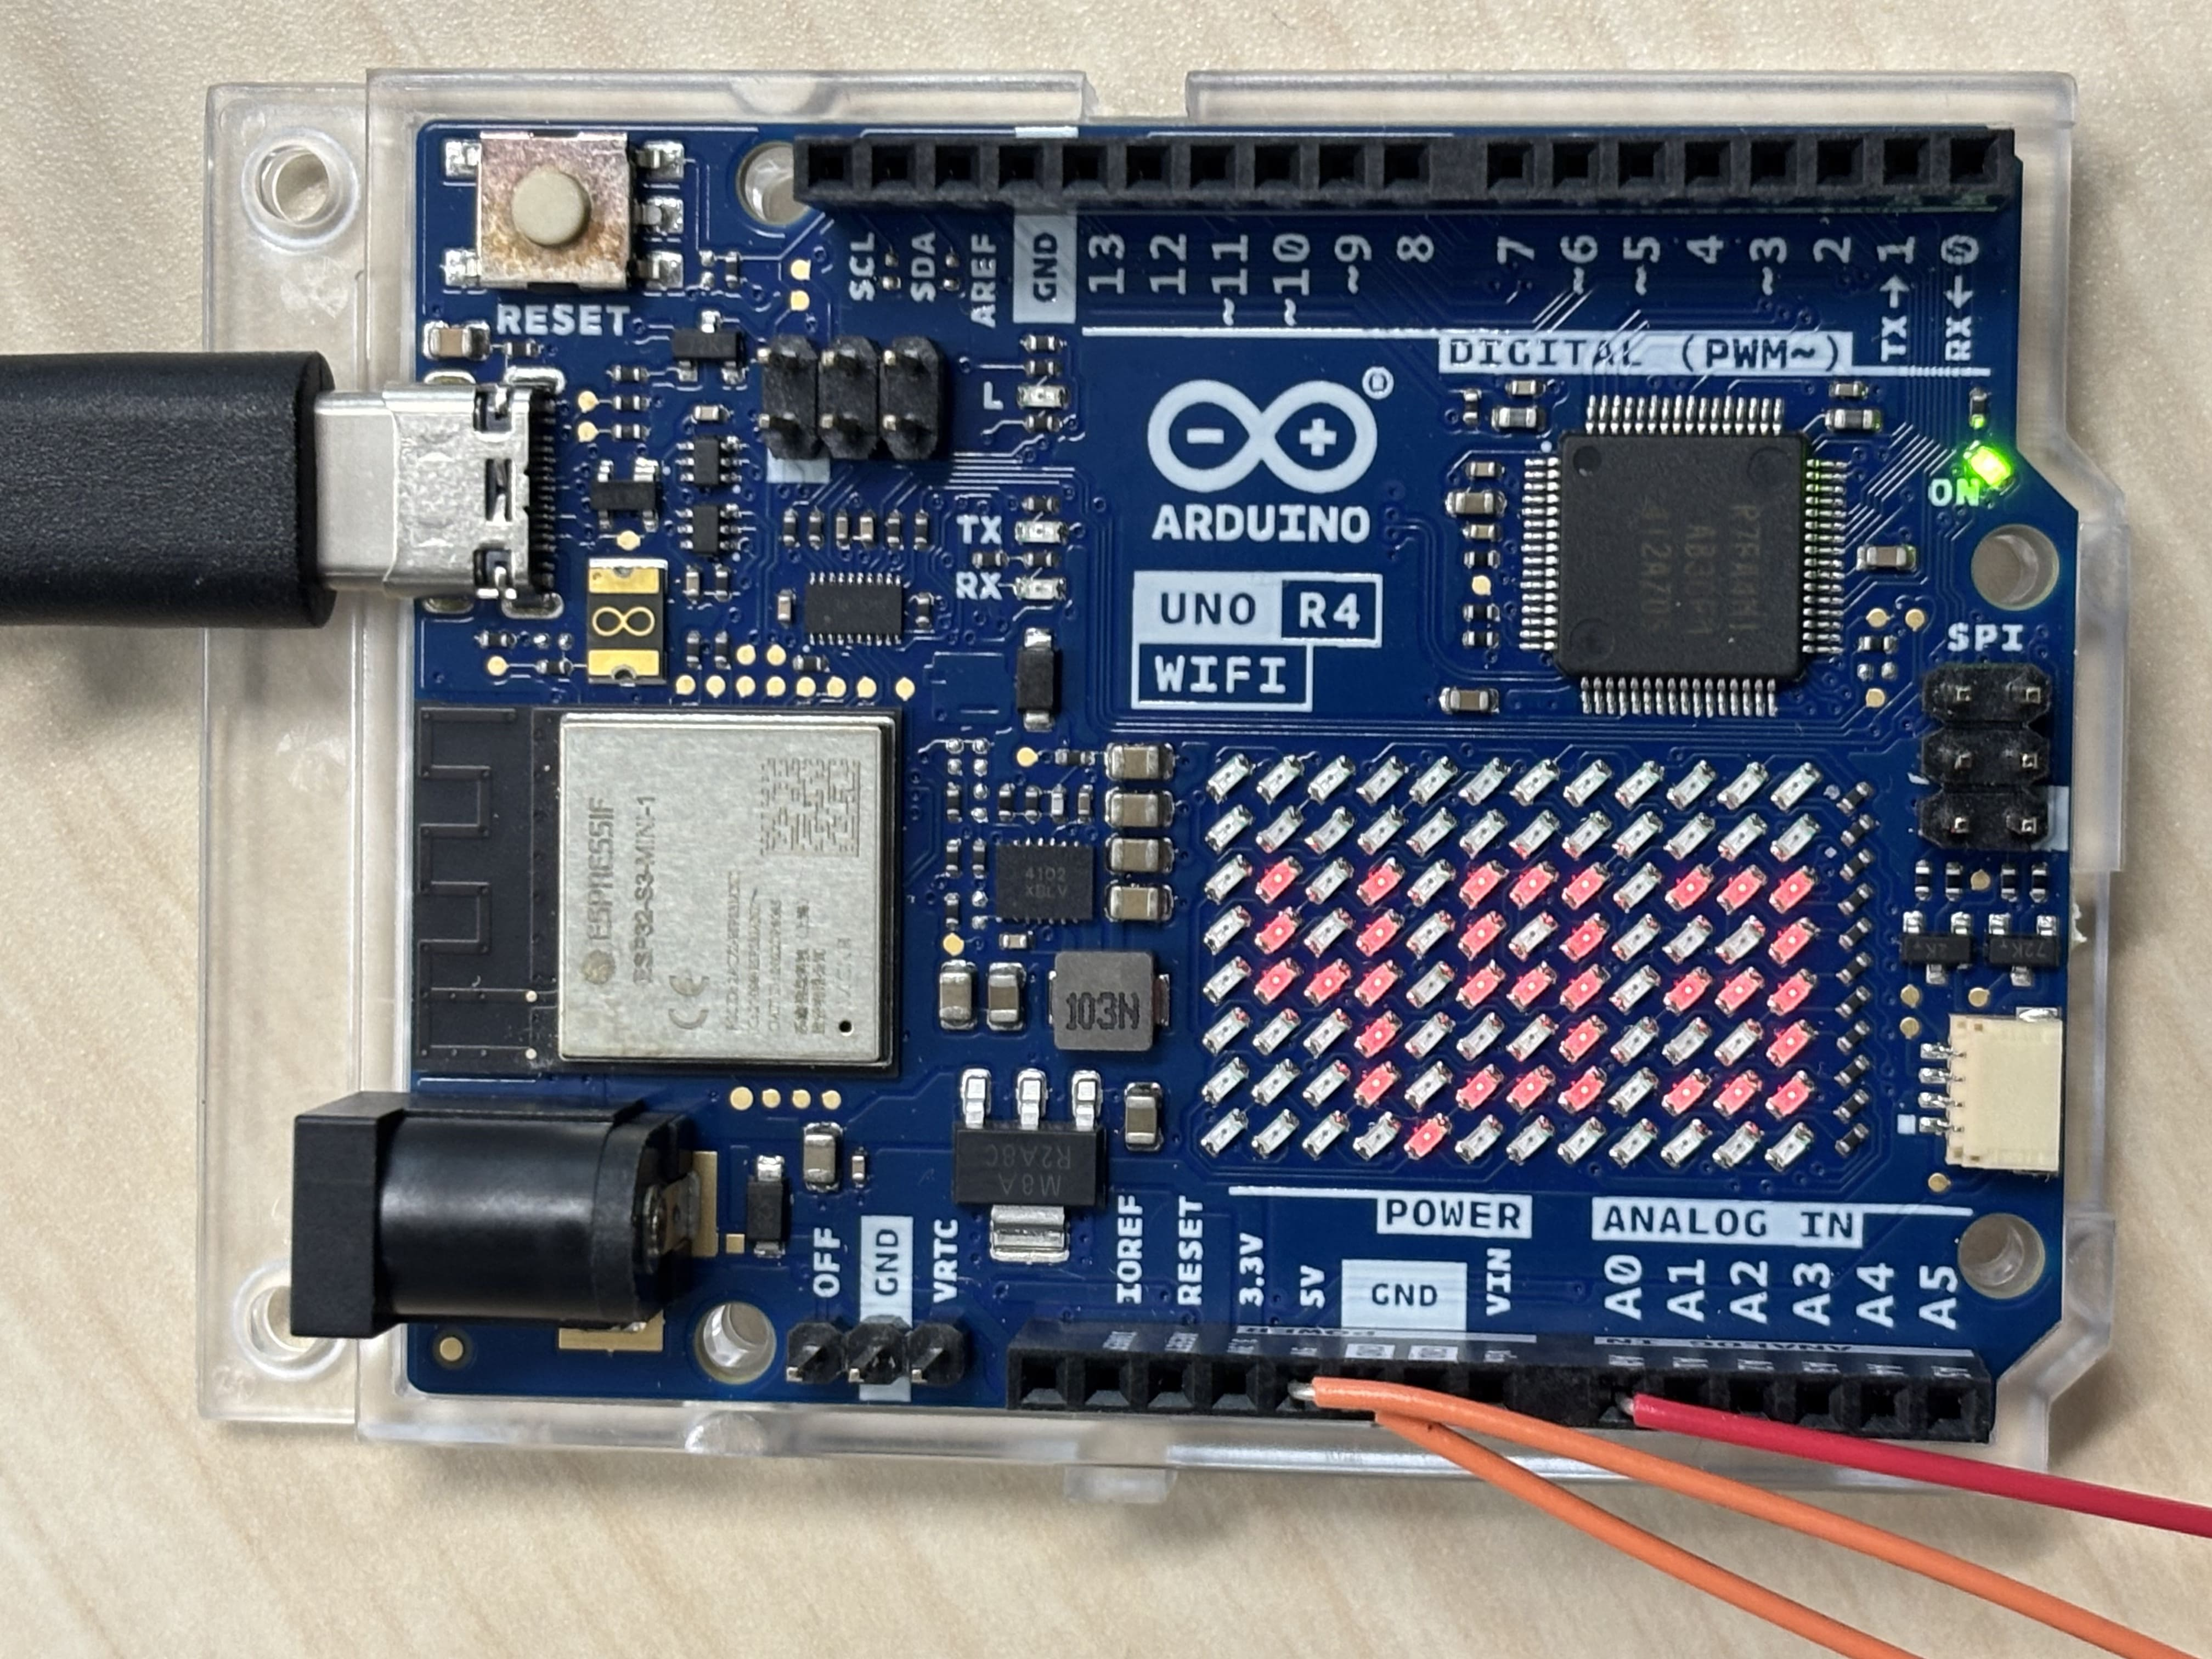
\includegraphics[width=0.8\linewidth]{fig_work_C/IMG_9242.jpg}
  \caption{電圧値を表示しているLEDマトリクスの例}
  \label{fig:C-1-LEDex}
\end{figure}

実験手順について説明する．まず，回路図を図\ref{fig:C-1-kairozu}に，実装した配線を図\ref{fig:C-1-kairo}に，使用した実験部品を表\ref{tab:C-1-1}に示す．
\begin{figure}[H]
  \centering
  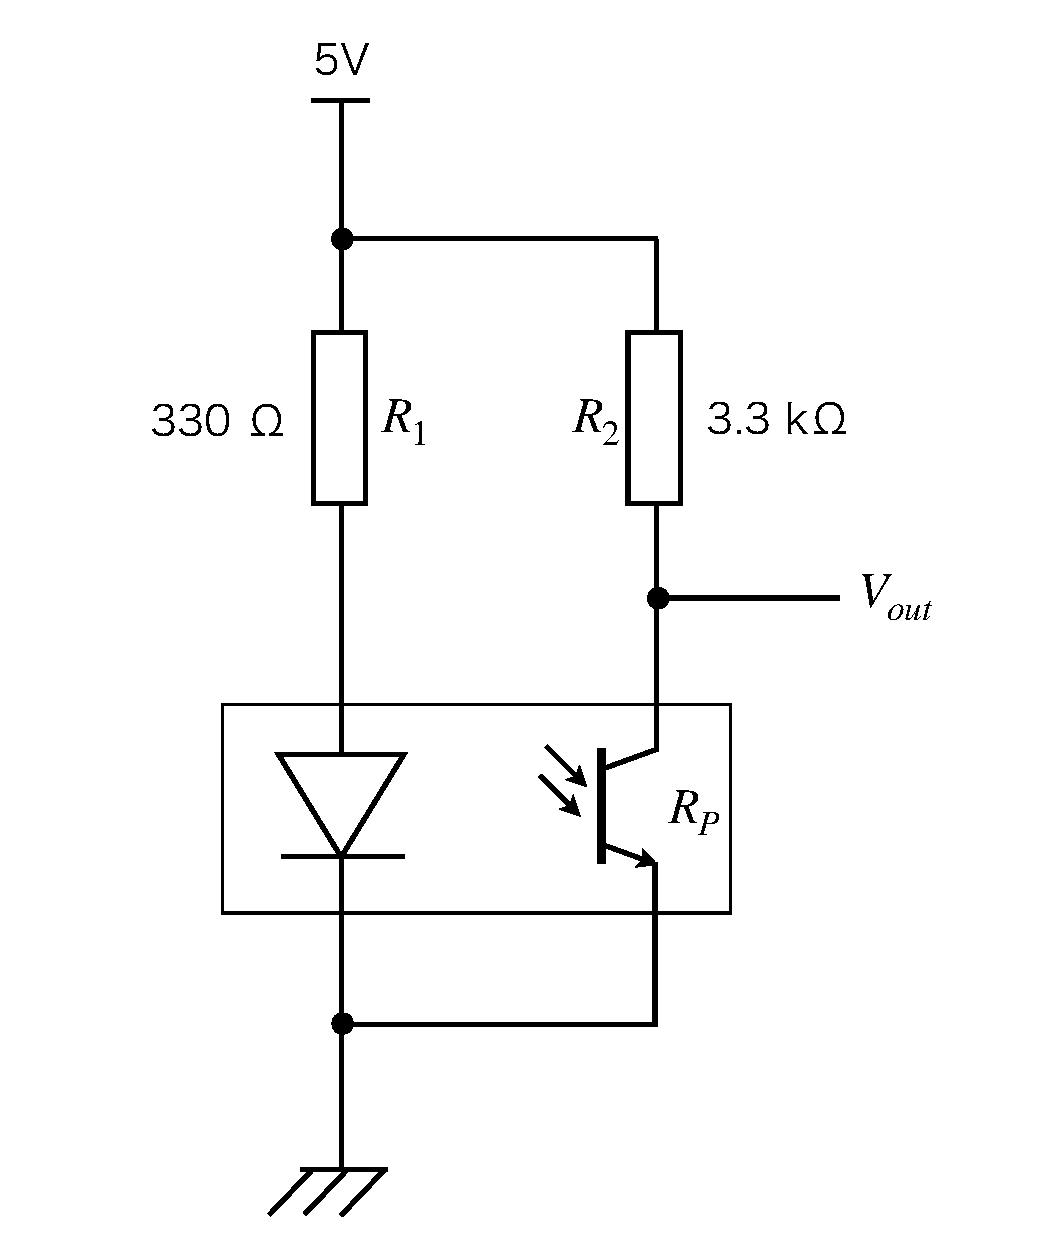
\includegraphics[width=0.7\linewidth]{fig_work_C/work_C-1_kairozu.pdf}
  \caption{フォトリフレクタを用いた分圧回路図}
  \label{fig:C-1-kairozu}
\end{figure}
\begin{figure}[H]
  \centering
  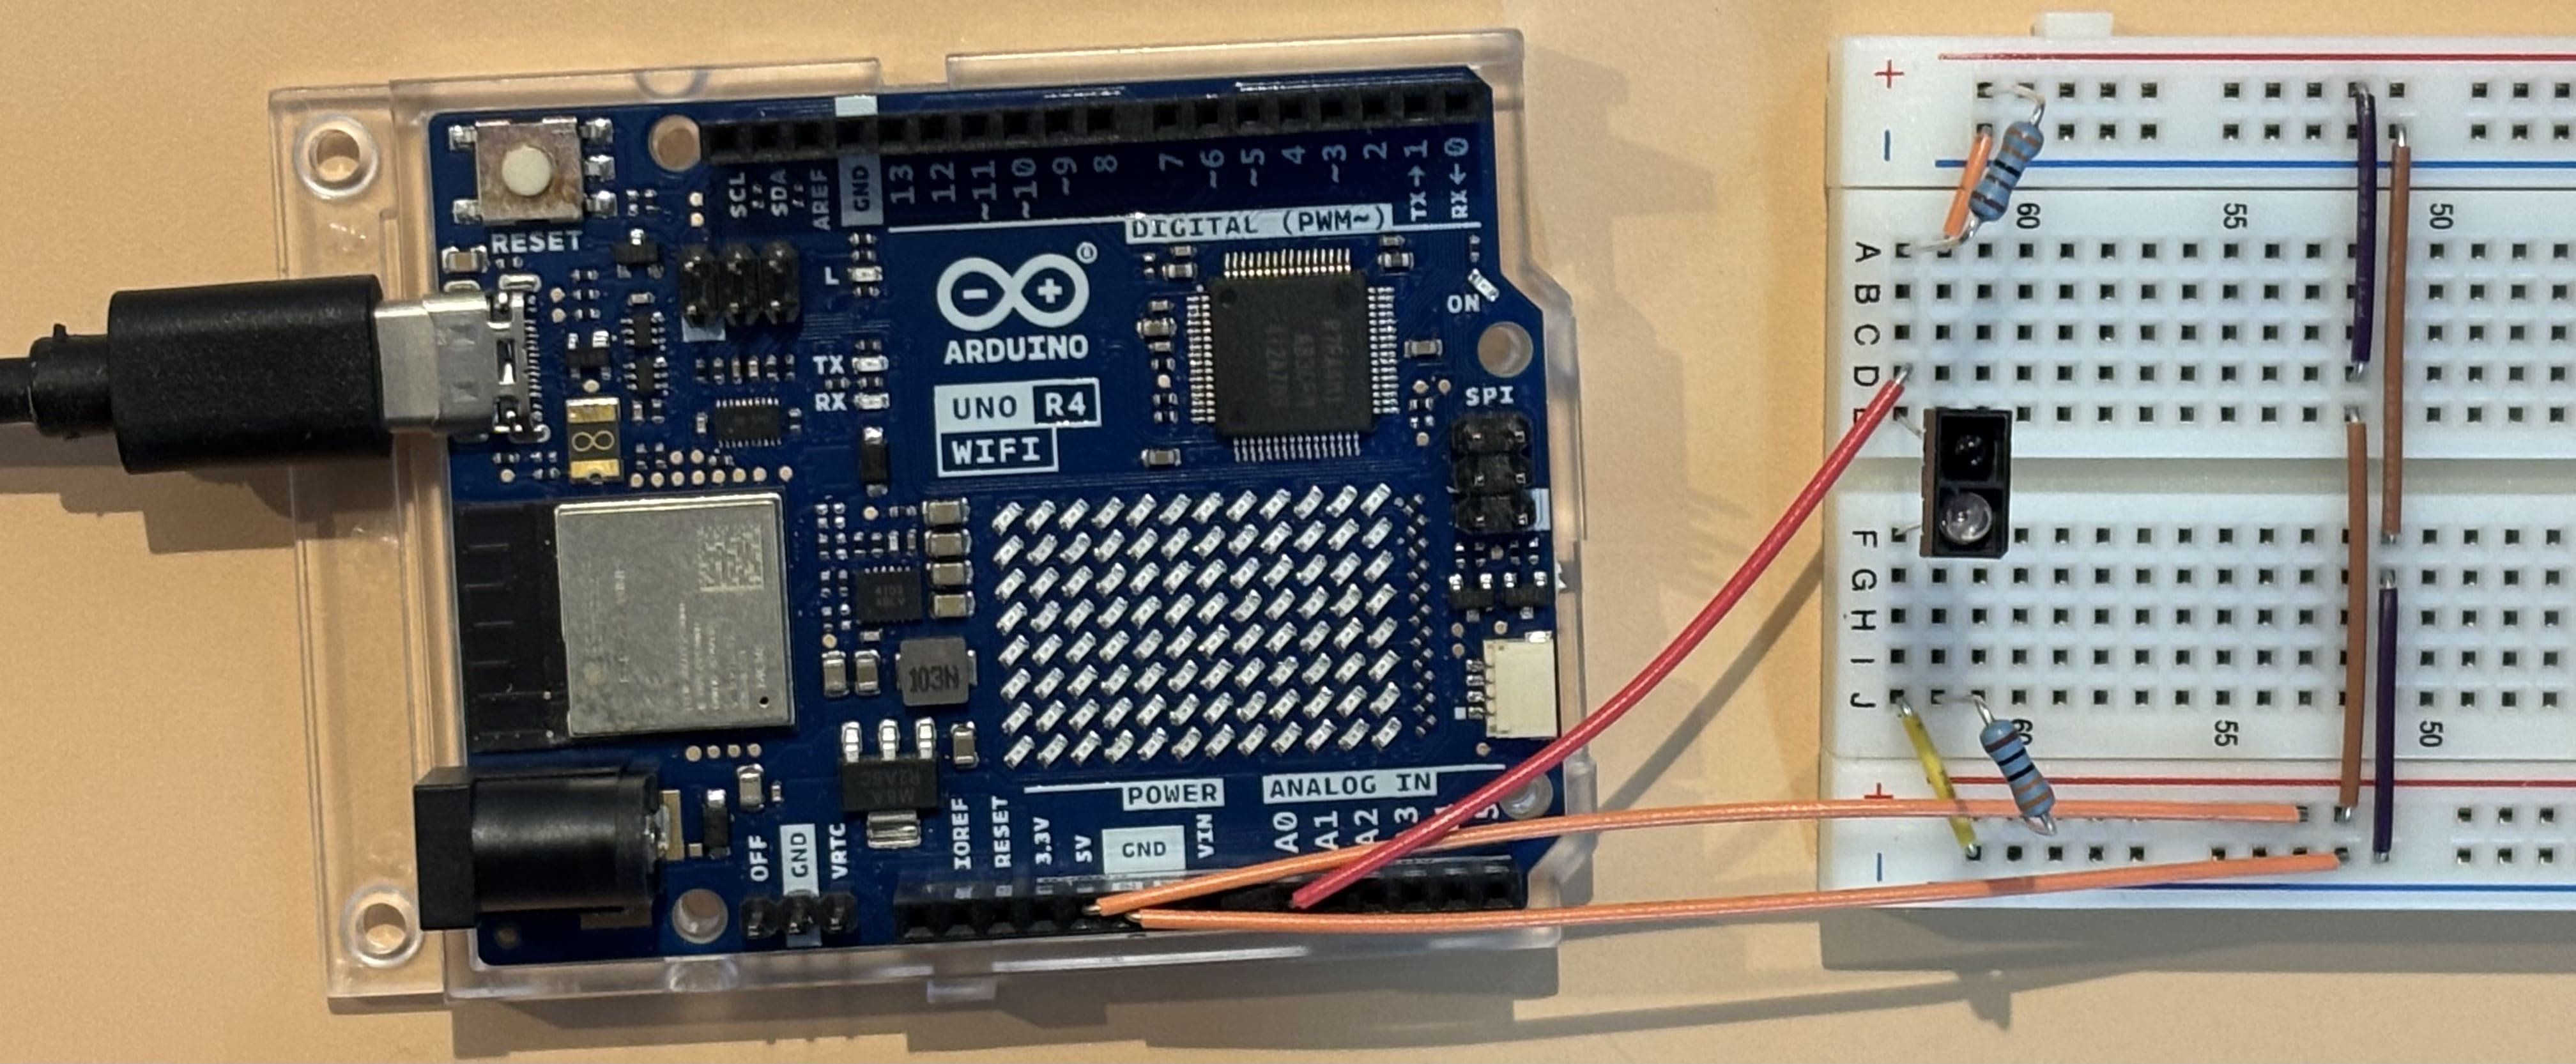
\includegraphics[width=0.9\linewidth]{fig_work_C/IMG_9240.jpg}
  \caption{フォトリフレクタを用いた分圧回路の配線}
  \label{fig:C-1-kairo}
\end{figure}
\begin{table}[H]
  \caption{使用した実験部品}
  \centering
  \begin{tabular}{|c|l|}
    \hline
    部品名 & 説明・備考 \\
    \hline \hline
    \multirow{2}{*}{Arduino Uno R4 WiFi} & A0ピンで3.3 k$\Omega$の抵抗器とフォトトランジスタの間の \\
     & アナログ値($V_{out}$)を読み取り，LEDマトリクスに結果を表示 \\
    \hline
    フォトリフレクタ & \multirow{2}{*}{遮蔽物からの反射光を検出し，距離に応じた電圧信号を出力} \\
    (LBR-127HLD)\cite{LBR-127HLD} & \\
    \hline
    抵抗器$R_1$(330 $\Omega$) & フォトリフレクタの赤外線LEDに接続する電流制限用の抵抗 \\
    \hline
    抵抗器$R_2$(3.3 k$\Omega$) & フォトリフレクタのフォトトランジスタに接続する抵抗 \\
    \hline
    ブレッドボード & 回路を実装するための土台 \\
    \hline
    ジャンパーワイヤ & Arduinoとブレッドボード，部品間の配線に使用 \\
    \hline
    PC(MacBook Pro) & 電源として使用 \\
    \hline
    USB Type-C & PCとArduinoを接続 \\
    \hline
  \end{tabular}
  \label{tab:C-1-1}
\end{table}
次に，フォトリフレクタと遮蔽物との距離を0.5 cmから5.0 cmまで0.5 cm間隔で変化させ，その際のA0ピンの電圧を測定した．
測定する際，距離を測るために定規を使用した．その計測の様子を図\ref{fig:C-1-keisoku}に示す．
\begin{figure}[H]
  \centering
  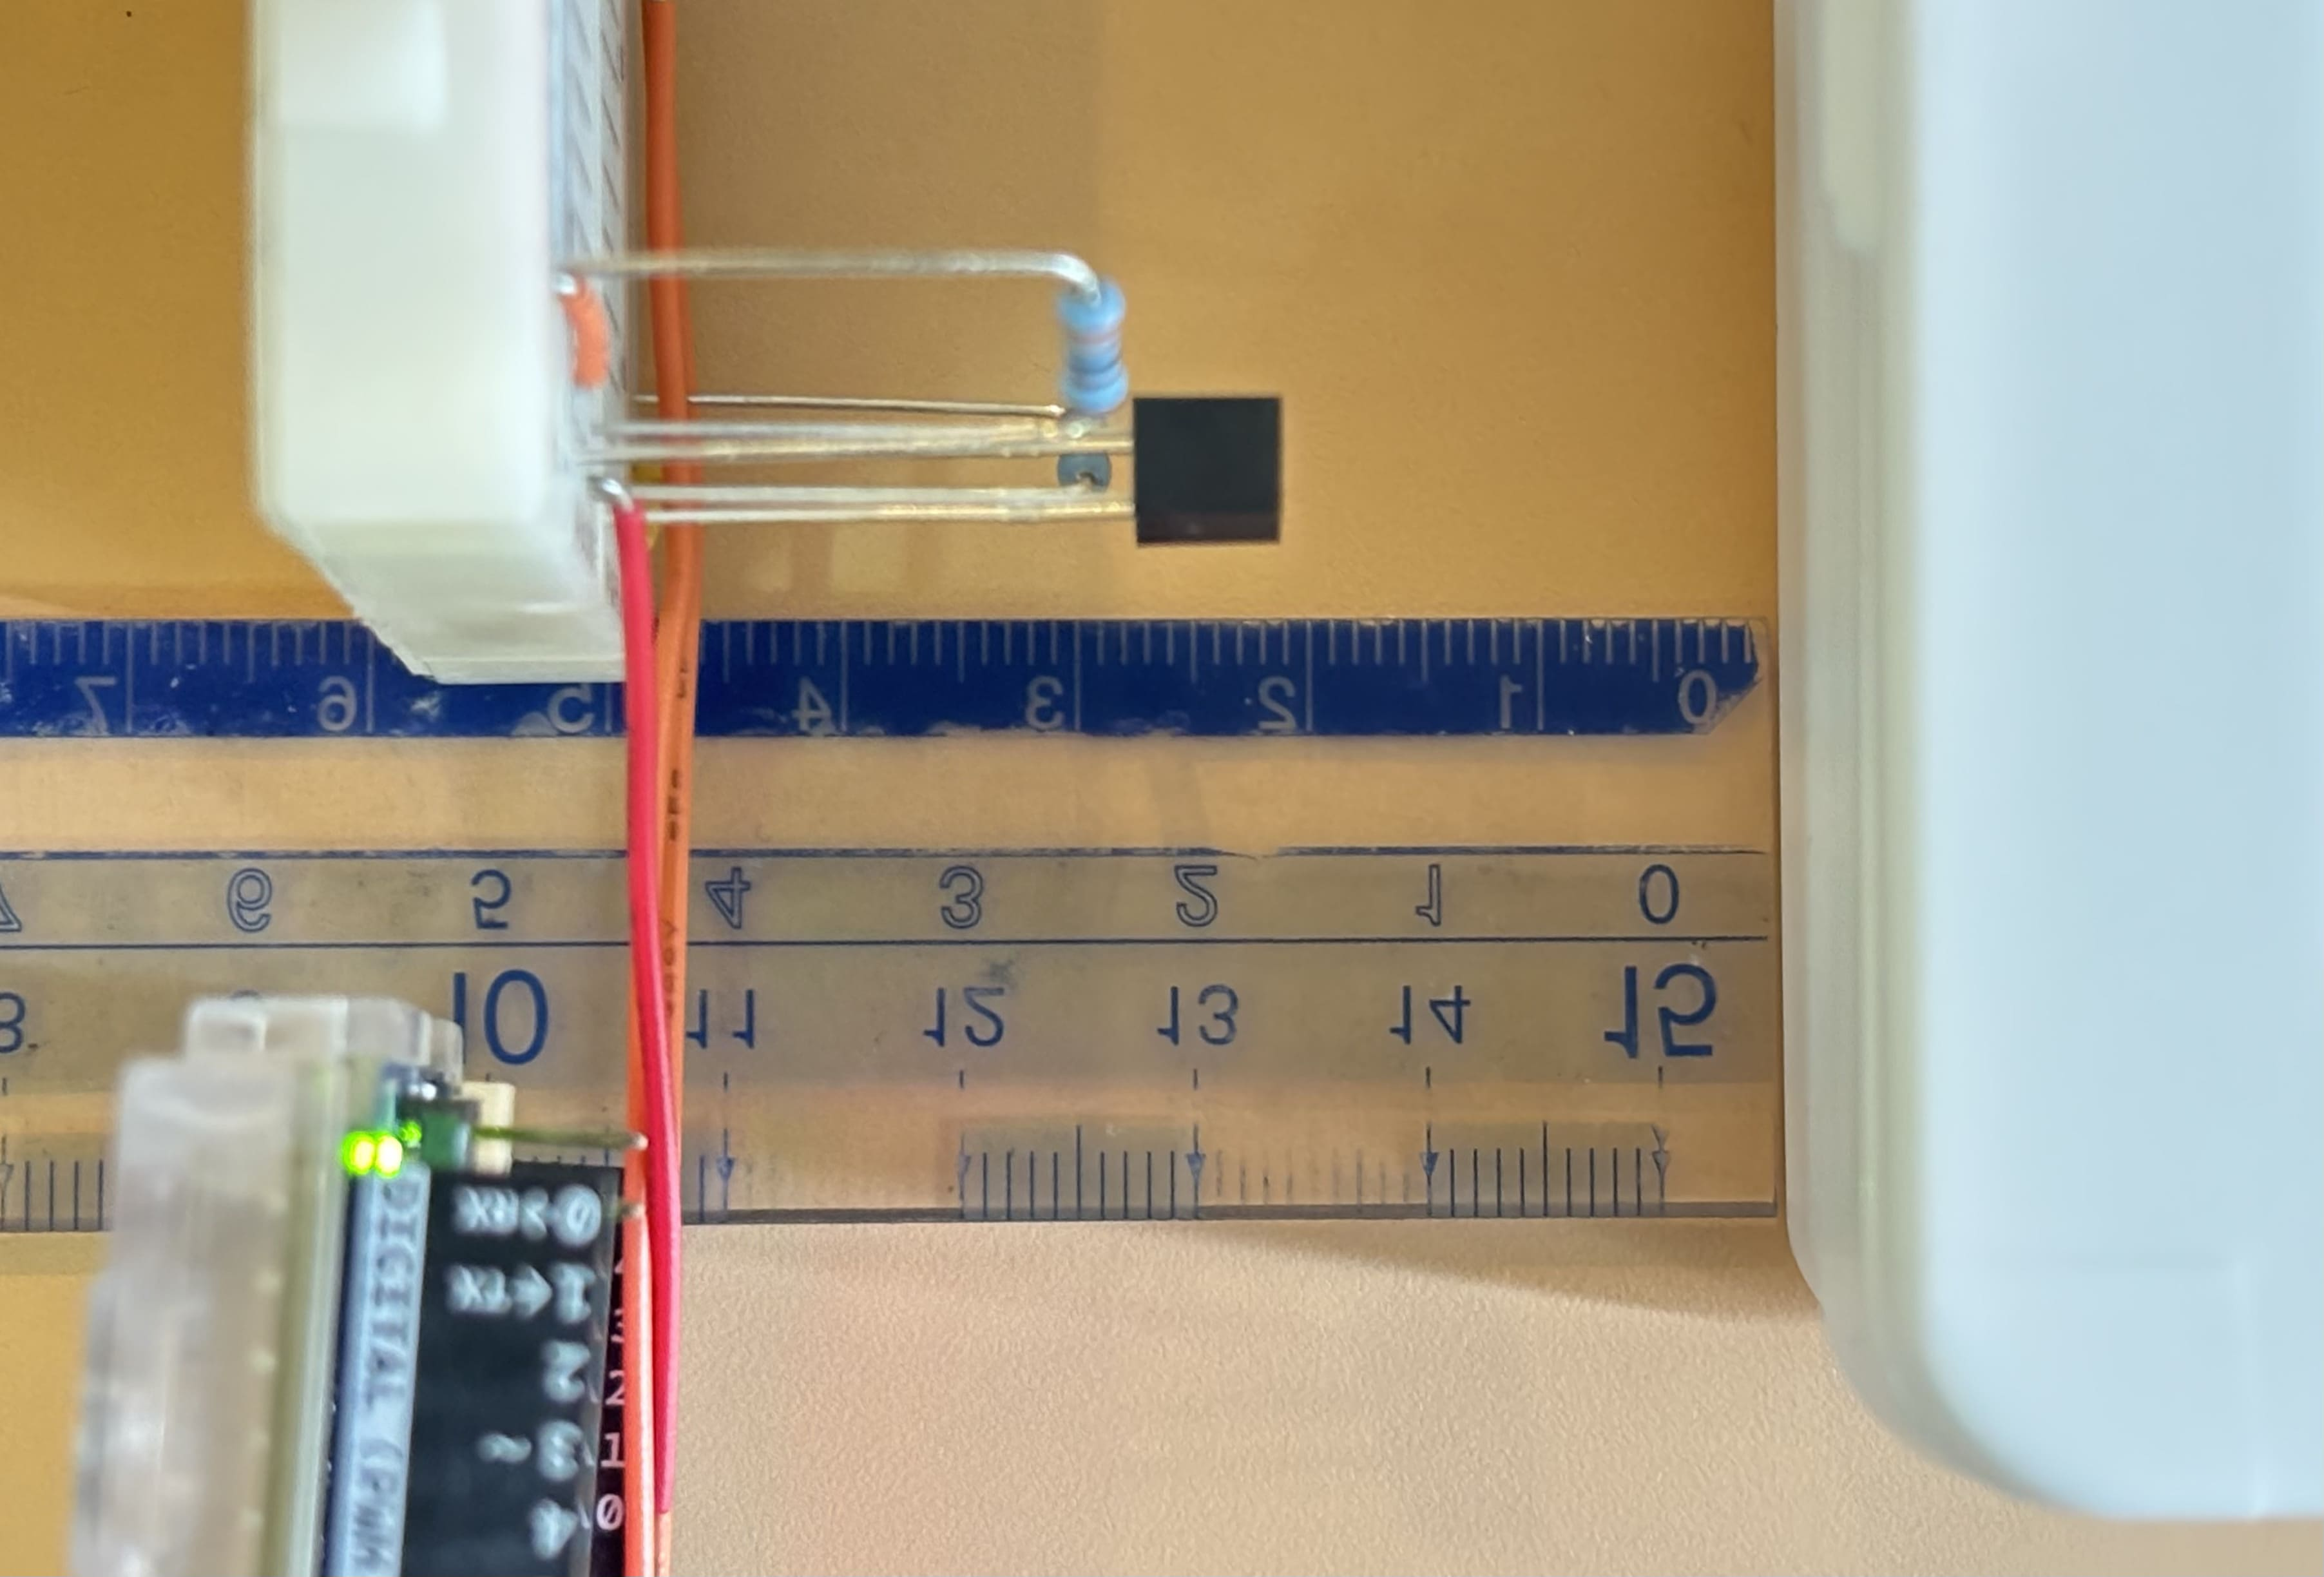
\includegraphics[width=0.9\linewidth]{fig_work_C/IMG_9238.jpg}
  \caption{フォトリフレクタと遮蔽物との距離の計測に定規を使用する様子}
  \label{fig:C-1-keisoku}
\end{figure}
測定した電圧値は遮蔽物との距離ごとに記録し，Pythonを用いて作成したフォトリフレクタと遮蔽物との距離と電圧値の関係を示すグラフで評価した．



\subsection{ワークC-2 ネットワークを介したデータの取得と分析}


本実習では，ArduinoをWebサーバとして機能させ，ネットワーク経由で測定データを取得するシステムを構築した．
ArduinoはWi-Fiモジュール(ESP32-S3)を利用してアクセスポイントモードで起動し，クライアントからのHTTPリクエスト待機状態にする．
クライアント側PCがPythonプログラムを用いてHTTP GETリクエストを送信すると，ArduinoはA0ピンで読み取った電圧値を返送する．
CdSセルは入射する光量によって抵抗値が増減するため\cite{workC_CdSセル}，この増減による電圧の変化を測定した．

回路図を図\ref{fig:C-2-kairozu}に，実装した配線を図\ref{fig:C-2-kairo}に，使用した実験部品を表\ref{tab:C-2-1}に示す．
\begin{figure}[H]
  \centering
  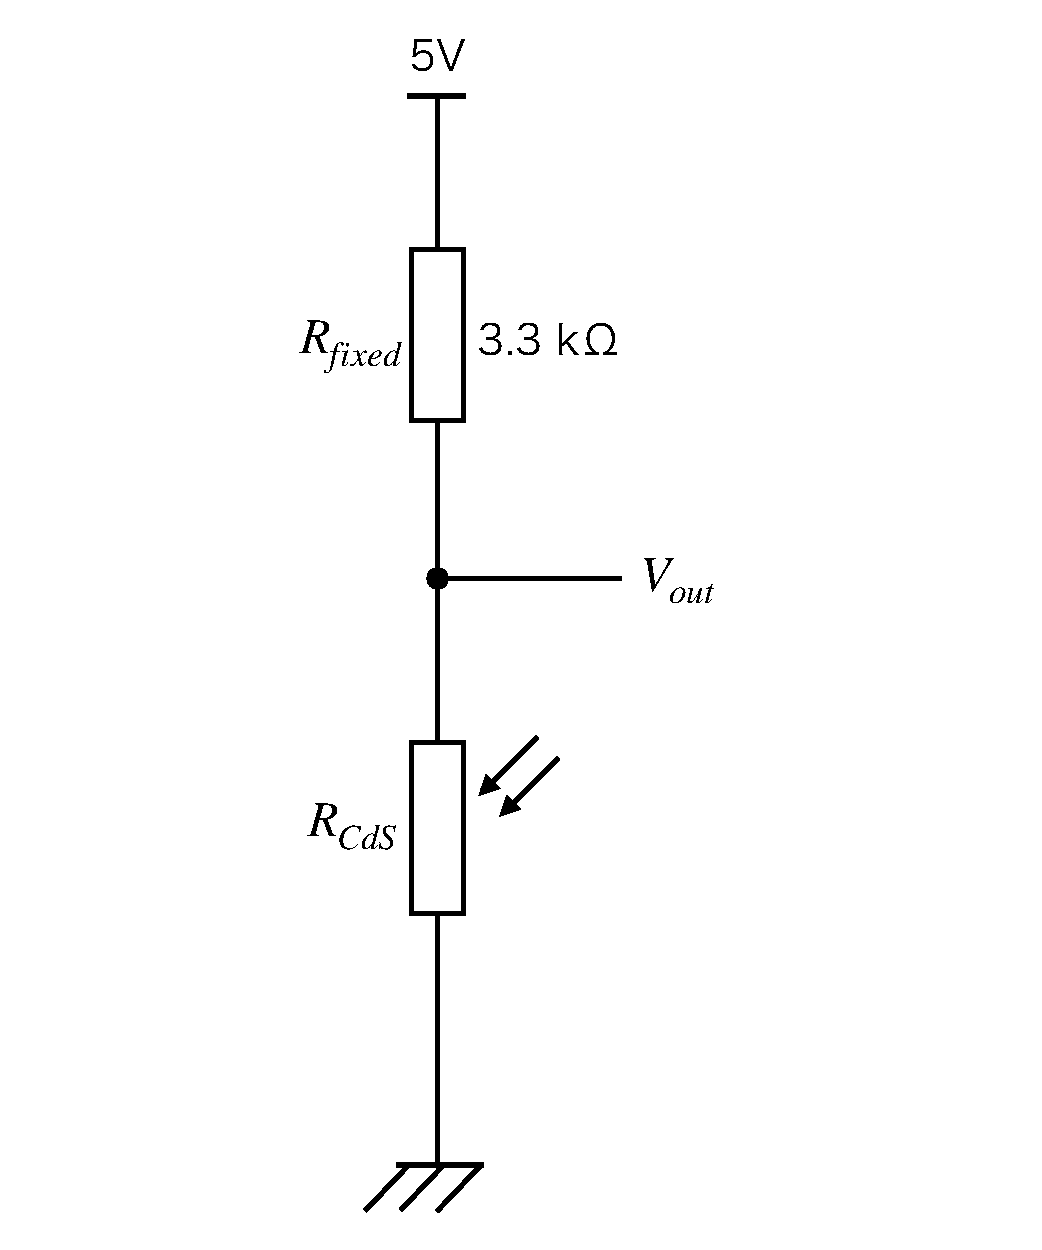
\includegraphics[width=0.7\linewidth]{fig_work_C/work_C-2_kairozu.pdf}
  \caption{CdSセルを用いた分圧回路図}
  \label{fig:C-2-kairozu}
\end{figure}
\begin{figure}[H]
  \centering
  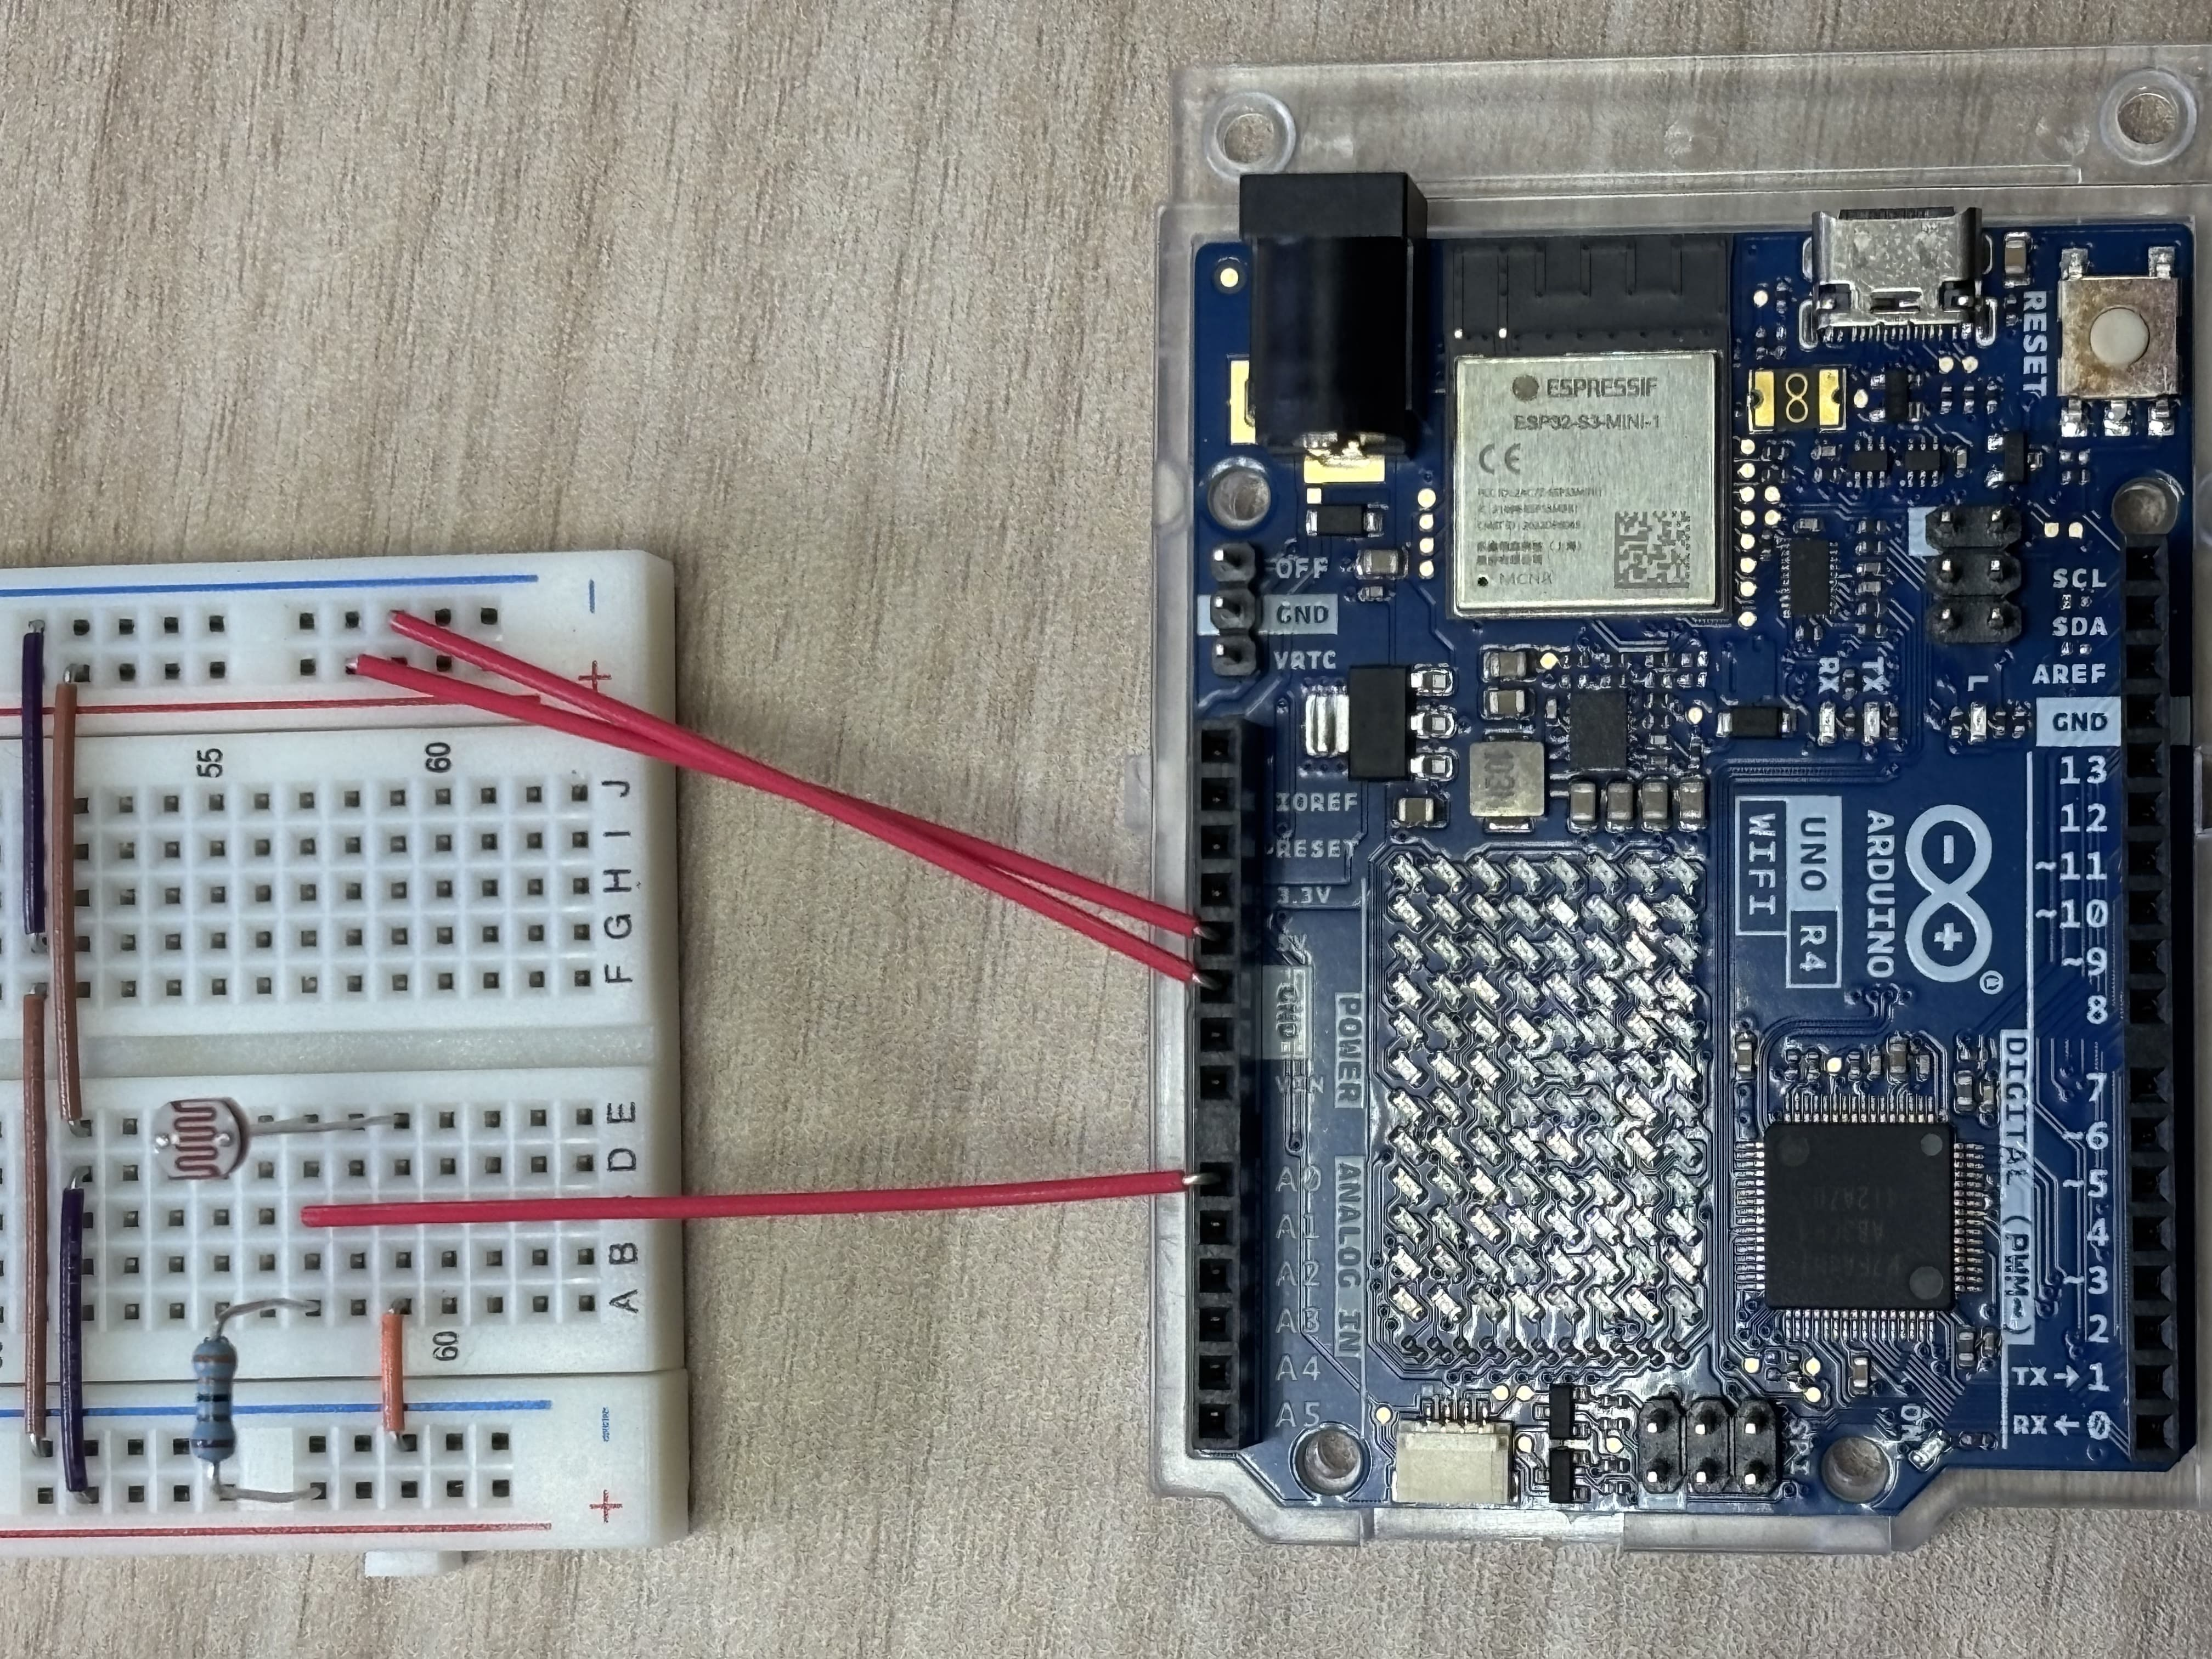
\includegraphics[width=0.8\linewidth]{fig_work_C/IMG_9271.jpg}
  \caption{CdSセルを用いた分圧回路の配線}
  \label{fig:C-2-kairo}
\end{figure}
\begin{table}[H]
  \caption{使用した実験部品}
  \centering
  \begin{tabular}{|c|l|}
    \hline
    部品名 & 説明・備考 \\
    \hline \hline
    \multirow{2}{*}{Arduino Uno R4 WiFi} & Webサーバとして機能し，A0ピンで電圧($V_{out}$)を \\
     & 測定してクライアント側PCへ送信 \\
    \hline
    CdSセル$R_{CdS}$ & \multirow{2}{*}{光の強度に応じて抵抗値が変化する光センサ} \\
    (GL3516)\cite{workC_GL3516} & \\
    \hline
    抵抗器$R_{fixed}$(3.3 k$\Omega$) & CdSセルと直列に接続し，分圧回路を構成するための抵抗 \\
    \hline
    ブレッドボード & 回路を実装するための土台 \\
    \hline
    ジャンパーワイヤ & Arduinoとブレッドボード，部品間の配線に使用 \\
    \hline
    クライアント側PC & Arduinoへリクエストを送信し，データを取得・記録 \\
    \hline
    USB Type-C & PCとArduinoを接続し，Arduinoに電力を供給 \\
    \hline
  \end{tabular}
  \label{tab:C-2-1}
\end{table}
\clearpage
実験手順として，以下の5つの条件で各20秒間ずつ電圧値を連続して測定した．
\begin{enumerate}
  \item センサ上部に何もない状態(天井の照明を受光)
  \item センサ上部約9.0 cmに手をかざした状態
  \item センサ上部約6.0 cmに手をかざした状態
  \item センサ上部約3.0 cmに手をかざした状態
  \item 再びセンサ上部に何もない状態
\end{enumerate}
クライアント側PCからは1秒ごとにリクエストを送信し，取得したデータを時系列データとしてCSVファイルに記録した．
その計測の様子を図\ref{fig:C-2-keisoku}に示す．
\begin{figure}[H]
  \centering
  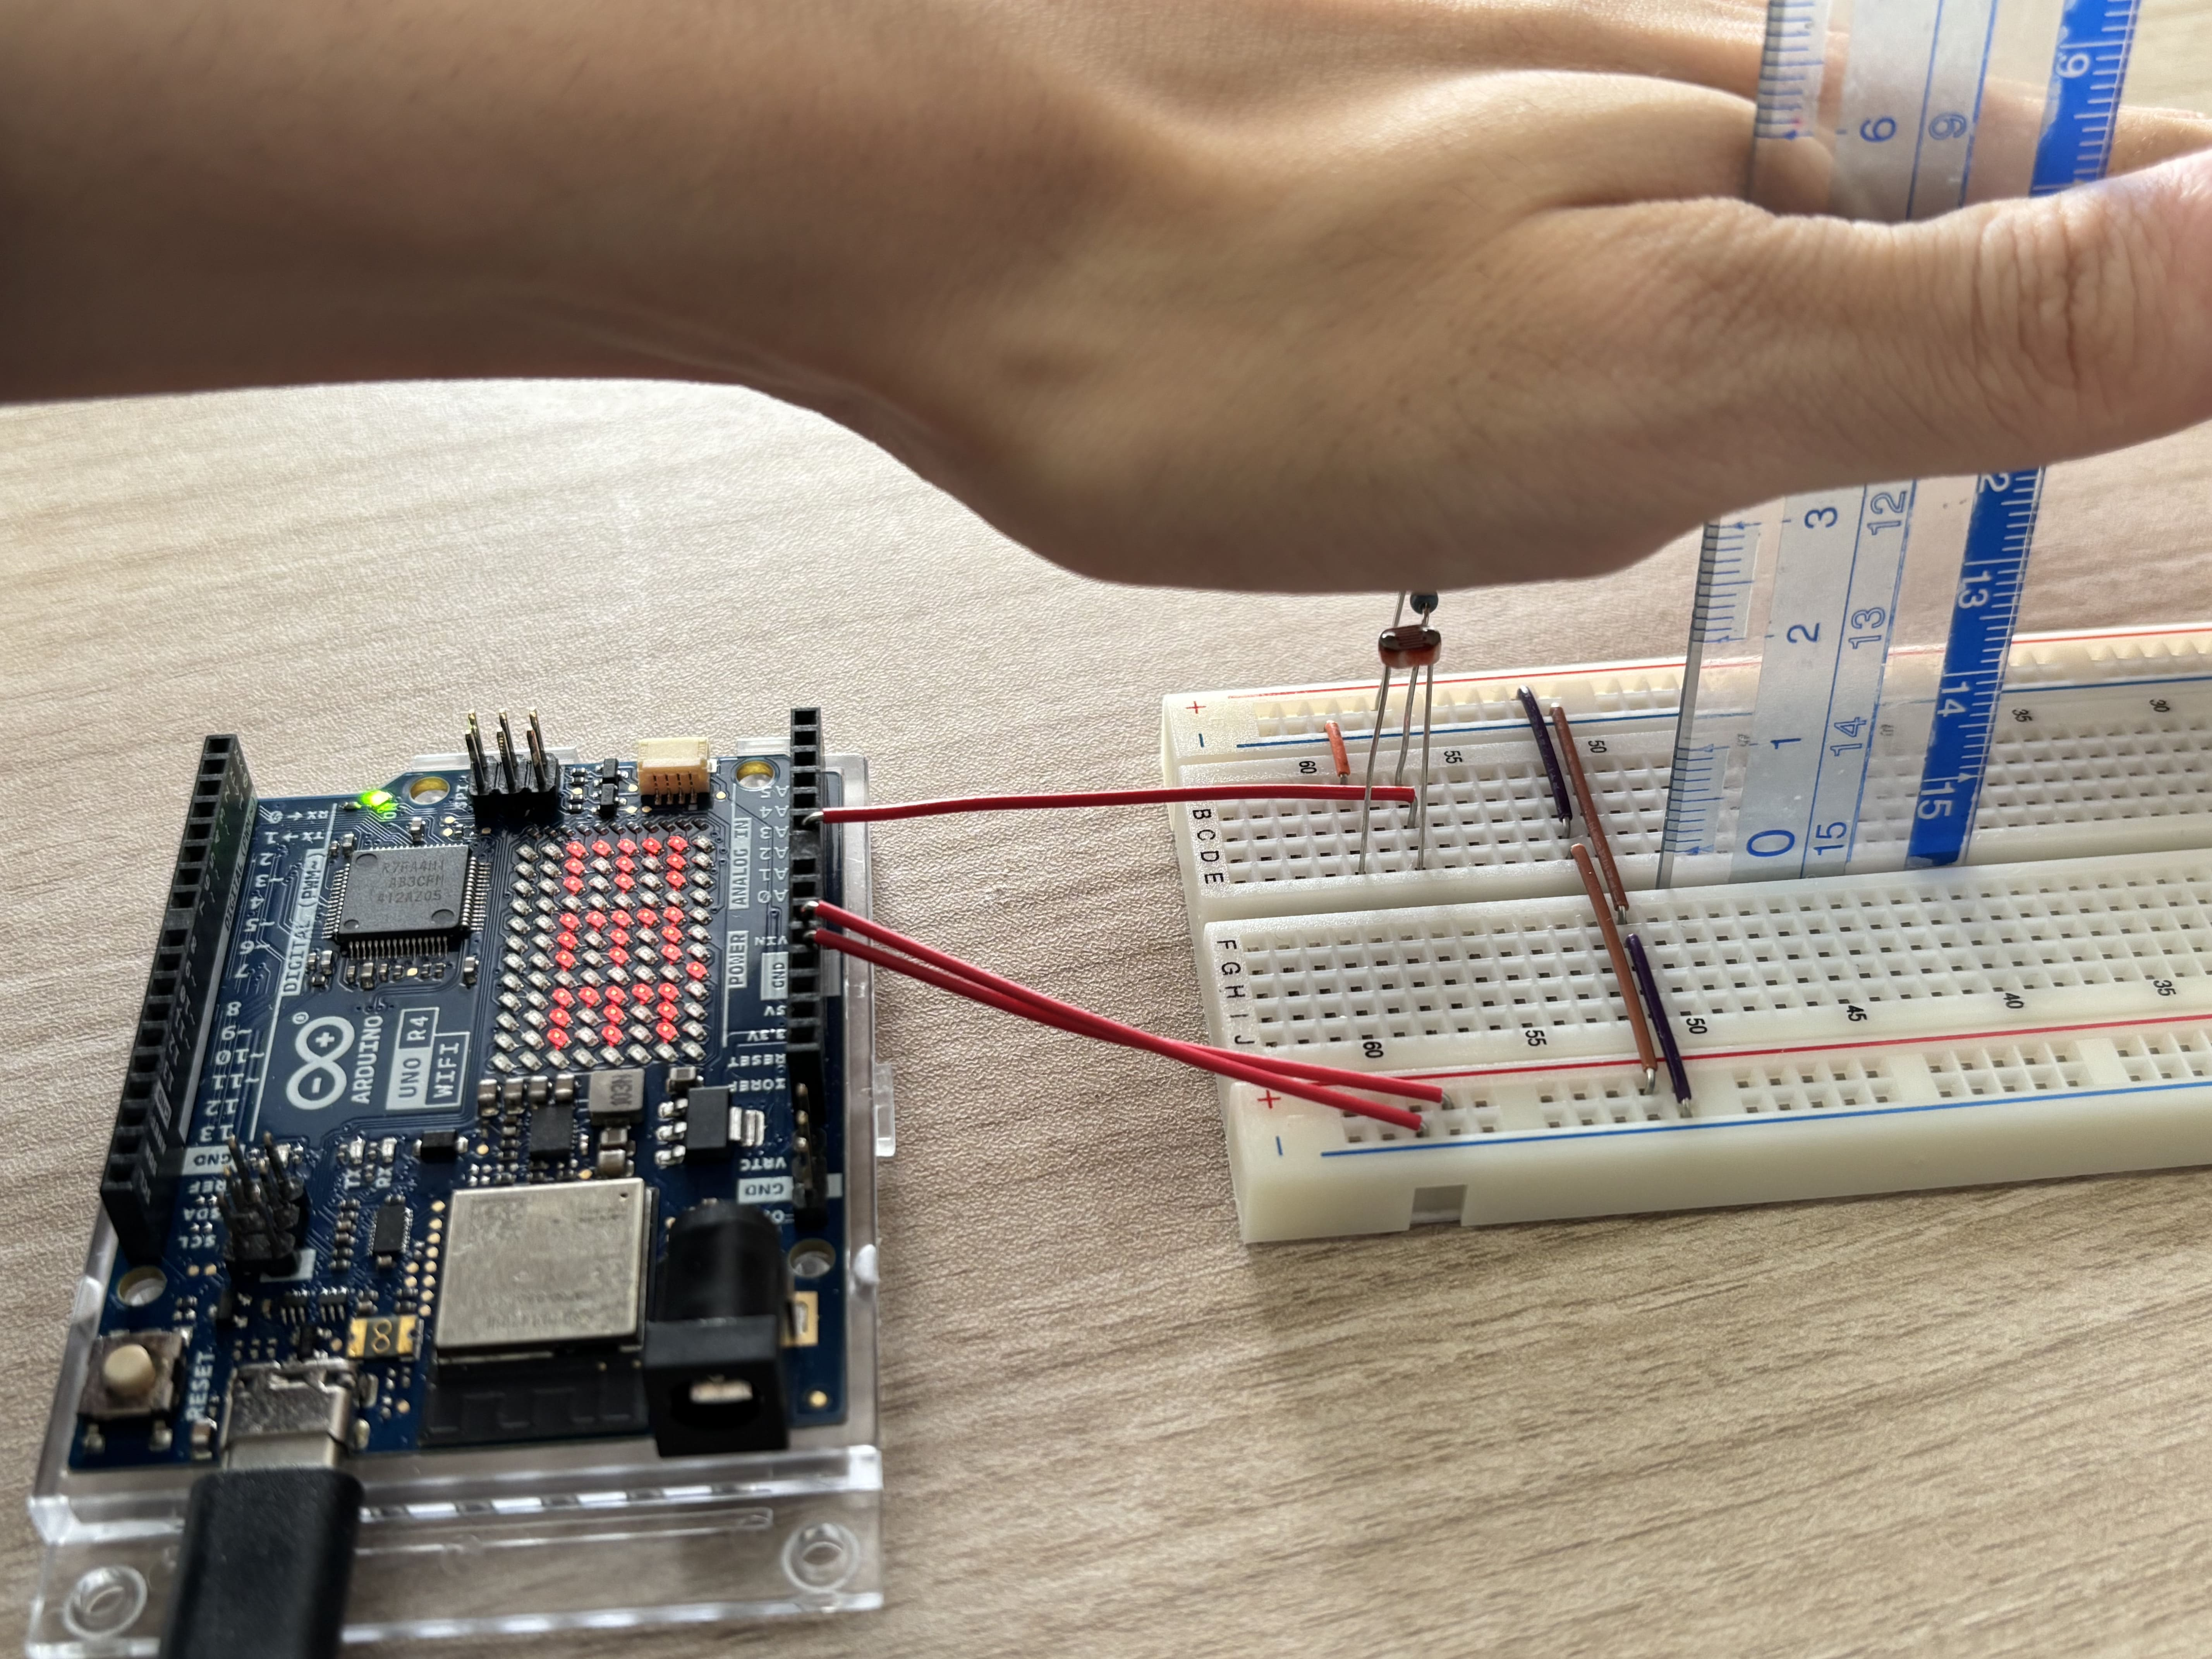
\includegraphics[width=0.8\linewidth]{fig_work_C/IMG_9293.jpg}
  \caption{CdSセルの上に定規を使用して手をかざす様子}
  \label{fig:C-2-keisoku}
\end{figure}
CSVファイルをもとに，Pythonを用いて作成した電圧値の変化を示すグラフで評価した．



\clearpage

\subsection{ワークC-3 時系列データの平滑化}


ワークC-2で取得した時系列データにはノイズが含まれるため，これを平滑化する処理の実装を行った．
本実習では，移動平均(Moving Average)および指数移動平均(Exponential Moving Average)の2種類の手法を用いて比較検証を行った．

移動平均は，直近$N$個のデータの単純平均を計算する手法である\cite{workC_MA}．
時刻$t$におけるデータ値を$x_t$とすると，移動平均値$y^{MA}_t$は式(\ref{eq:MA})で表される．
\begin{equation}
  y^{MA}_t = \frac{x_t + x_{t-1} + \dots + x_{t-N+1}}{N} \label{eq:MA}
\end{equation}
指数移動平均は，過去のデータほど重みを指数関数的に減少させ，直近のデータを重視する手法である\cite{workC_MA}．
平滑化係数を$\alpha = \frac{2}{N+1}$とすると，指数移動平均値$y^{EMA}_t$は式(\ref{eq:EMA})で表される．
\begin{equation}
  y^{EMA}_t = \alpha x_t + (1 - \alpha) y^{EMA}_{t-1} \label{eq:EMA}
\end{equation}

本実習では，ウィンドウサイズを$N=5$，$N=10$とし，移動平均の計算にはPythonのpandasライブラリのrolling()関数を用い，
指数移動平均の計算にはewm()関数を用いて計算を行った．
その後，元のデータと比較するグラフを作成して評価した．


\clearpage \section{結果} 
%実験から得られた結果について記述し，その中で読者の興味を引く結果がどれであり，それが何であるかを述べる．
%グラフや表にまとめるべきデータがあれば適切に図表として示すこと．
%本節の目的は図表を活用して要点を簡潔にまとめることであり，図表を文章にするのではない点に注意する．

\subsection{ワークC-1 LEDマトリクスの活用}
本実習では，フォトリフレクタと遮蔽物との距離を変化させ，電圧値との関係を示すグラフを作成した．
ArduinoのLEDマトリクスに表示された結果を表\ref{tab:C-1-result1}に示す．
\begin{table}[H]
  \caption{フォトリフレクタと遮蔽物との距離と電圧値}
  \centering
  \begin{tabular}{|c|c|c|c|c|c|c|c|c|c|c|}
    \hline
    距離 [cm] & 0.5 & 1.0 & 1.5 & 2.0 & 2.5 & 3.0 & 3.5 & 4.0 & 4.5 & 5.0 \\
    \hline
    電圧値 [V] & 2.20 & 3.37 & 4.11 & 4.42 & 4.57 & 4.70 & 4.74 & 4.76 & 4.78 & 4.79 \\
    \hline
  \end{tabular}
  \label{tab:C-1-result1}
\end{table}
表\ref{tab:C-1-result1}の数値から作成したグラフを図\ref{fig:C-1-result2}に示す．
\begin{figure}[H]
  \centering
  \includegraphics[width=0.6\linewidth]{../work/result_C1.png}
  \caption{フォトリフレクタと遮蔽物との距離と電圧値の関係}
  \label{fig:C-1-result2}
\end{figure}
横軸はフォトリフレクタと遮蔽物との距離 [cm]，縦軸は電圧 [V]を表している．
遮蔽物との距離が0.5 cmから2.5 cmの間では距離が離れるにつれて電圧値が急激に上昇し，
3.0 cm～5.0 cmでは電圧値の上昇が緩やかになり，約4.8 Vに収束する傾向が確認された．



\clearpage

\subsection{ワークC-2 ネットワークを介したデータの取得と分析}
CdSセルを用いて照度変化に伴う電圧の時間変化を測定した結果を図\ref{fig:C-2-result}に示す．
\begin{figure}[H]
  \centering
  \includegraphics[width=0.8\linewidth]{../work/result_C2.pdf}
  \caption{照度変化に伴う電圧の時間変化(生データ)}
  \label{fig:C-2-result}
\end{figure}
横軸は経過時間 [s]，縦軸は電圧 [V]を表している．
手をかざしていない状態(0～20秒，80～100秒)では約2.4 Vで安定しているが，
手をかざしてセンサへの光を遮ると電圧が上昇することが確認された．
また，手との距離が9.0 cm，6.0 cm，3.0 cmと近づくにつれて(20～80秒)，階段状に電圧値が増加する傾向が得られた．
一方で，電圧が一定となるべき区間においても，微小な電圧の振動(ノイズ)が観測された．



\subsection{ワークC-3 時系列データの平滑化}
ワークC-2で得られたデータに対し，ウィンドウサイズを$N=5$として移動平均および指数移動平均を適用した結果を図\ref{fig:C-3-result}に示す．
\begin{figure}[H]
  \centering
  \includegraphics[width=0.945\linewidth]{../work/result_C3.png}
  \caption{ウィンドウサイズを$N=5$とした平滑化手法による波形の違い}{(上：生データ，中：移動平均，下：指数移動平均)}
  \label{fig:C-3-result}
\end{figure}
上段は元の生データ，中段は移動平均，下段は指数移動平均の結果であり，横軸は経過時間 [s]，縦軸は電圧 [V]を表している．
いずれの手法においても，生データで見られた微細なノイズが低減され，波形が滑らかになっていることが確認できる．
特に，電圧が急激に変化するタイミング(手が移動するとき)において，移動平均と指数移動平均で生データに対する追従性に違いが見られた．

ウィンドウサイズを$N=10$として作成したグラフを図\ref{fig:C-3-result-N10}に示す．
\begin{figure}[H]
  \centering
  \includegraphics[width=0.92\linewidth]{../work/result_C3_N=10.png}
  \caption{ウィンドウサイズを$N=10$とした平滑化手法による波形の違い}{(上：移動平均，下：指数移動平均)}
  \label{fig:C-3-result-N10}
\end{figure}
上段は移動平均，下段は指数移動平均の結果であり，横軸は経過時間 [s]，縦軸は電圧 [V]を表している．



\clearpage \section{考察} 
%本ワークで得られた結果について考察する．
%例えば，以下のように記述する．

%（例）本ワーク○○では○○の結果が得られたが，これは理論値と比較して○○な結果である．これは○○が原因であると考えられる．

\subsection{ワークC-1 LEDマトリクスの活用}

本実習では，フォトリフレクタと遮蔽物との距離が電圧値に与える影響を検証した．
図\ref{fig:C-1-result2}に示すグラフでは，距離が0.5 cmから2.5 cmの間で電圧値が急上昇し，3.0 cm以降は約4.80 Vで収束する傾向が確認された．
この特有のグラフ形状は，光の強さが距離に応じて減衰する逆二乗の法則と\cite{workC_逆二乗の法則}，
センサ回路の電気的な特性を決定づけるオームの法則(式(\ref{eq:オームの法則}))によって説明できる\cite{workC_オームの法則}．
\begin{equation}
  V = I \times R \label{eq:オームの法則}
\end{equation}

まず，A0ピンで観測される電圧は，図\ref{fig:C-1-kairozu}に示す回路によって決定される．
この回路は，3.3 k$\Omega$の固定抵抗($R_2$)と，フォトリフレクタのフォトトランジスタ($R_P$)が直列に接続された分圧回路である\cite{workC_分圧回路}．
フォトトランジスタは，受光する光の強さに応じて抵抗($R_P$)が変化する可変抵抗として機能する．
A0ピンは，この$R_P$にかかる電圧($V_{out}$)を測定しており，その値はオームの法則に基づき，式(\ref{eq:A0電圧})の関係で表される．
\begin{equation}
  V_{out} = V_{CC} \times \frac{R_P}{R_2 + R_P} \label{eq:A0電圧}
\end{equation}

次に，受光する光の強さは逆二乗の法則に従う．
センサのLEDから放たれた赤外線は，遮蔽物に当たって反射し，フォトトランジスタに戻ってくる．
光は往復で距離の影響を受けるため，受光する光の強さは距離の二乗に反比例して急激に減少する．
この法則が，図\ref{fig:C-1-result2}のグラフのような形状を生み出す要因である．

これら2つの法則を組み合わせると，観測された図\ref{fig:C-1-result2}のグラフの傾向が説明できる．
遮蔽物が近い場合，反射光が強く，フォトトランジスタの抵抗値($R_P$)は低くなる．
分圧回路の特性により，$V_{out}$はGND側に引かれ，表\ref{tab:C-1-result1}では0.5 cmのとき2.20 Vという低い電圧となった．
遮蔽物を遠ざけると，逆二乗の法則に従い反射光が急激に減少し，$R_P$は高くなる．
これにより，$V_{out}$は分圧回路の特性に従って急激に上昇する．
そして，3.0 cm付近で反射光がほぼ0に近くなると，$R_P$は最大値に近くなり，それ以上はほとんど増加しなくなる．
その結果，$V_{out}$は電源電圧(5V)に近い約4.8 Vで収束したと考えられる．

以上の考察から，センサの出力電圧はフォトトランジスタが受光する赤外線の量によって決定されることがわかった．
本実習では距離を変数としたが，受光量は遮蔽物の反射率にも依存する．
したがって，本センサ回路の出力は，対象物との距離だけでなく，対象物の赤外線反射率にも強く関係していると考察できる．
この特性を利用し，一定の電圧を閾値とすることで，物体の有無を検知する非接触のスイッチへの応用が可能であると考えられる．




\subsection{ワークC-2 ネットワークを介したデータの取得と分析}

ワークC-2では，CdSセルを用いた回路の出力をネットワーク経由で連続的に測定し，光量の変化に伴う電圧値の変動を検証した．

まず，図\ref{fig:C-2-result}に示すように，手を近づけてセンサの照度が低下すると電圧値が上昇する結果が得られた．
この現象は，CdSセルの特性と，実験で用いた分圧回路の特性によって説明される．
CdSセルは，光のエネルギーを吸収することで内部の電子が増加し，電気抵抗が減少する性質を持つ\cite{workC_CdSセル}．
これにより，手を近づけてセンサへの入射光量が減少すると，CdSセルの内部抵抗($R_{CdS}$)が増加する．
図\ref{fig:C-2-kairozu}の回路は，固定抵抗($R_{fixed}$)と$R_{CdS}$が直列に接続された分圧回路であり，
A0ピンで測定される電圧($V_{out}$)は式(\ref{eq:A0電圧CdS})によって決定される\cite{workC_分圧回路}．
\begin{equation}
  V_{out} = V_{CC} \times \frac{R_{CdS}}{R_{fixed} + R_{CdS}} \label{eq:A0電圧CdS}
\end{equation}
この関係に基づき，照度低下によって$R_{CdS}$が増加すると，測定点($V_{out}$)にかかる電圧が上昇する．
CdSセルの性質により，手を近づけることによる照度低下は$R_{CdS}$の増加し，それに伴い分圧回路の特性によって$V_{out}$が上昇する．
その結果，図\ref{fig:C-2-result}のような電圧変化が観測されたと考察できる．

次に，20秒ごとの手の位置変更による大きな電圧変化のほかにも，電圧値に小さな変動が見られた．
この小さな変動の要因を考察する．
第一に，測定環境の照明の光のちらつきが，CdSセルでノイズとして検出された可能性が考えられる．
第二に，回路を流れる電流によるノイズや，Arduinoにおけるデジタル化に伴う誤差など，測定過程で生じるノイズが重畳している可能性がある．
第三に，一定の距離で手を静止させているつもりでも，測定者の微細な震えによって，センサ上を通過する光量がわずかに変動したこともノイズの一因として挙げられる．

続いて，手の位置を安定させる以外の方法で電圧値の小さな変動を低減する方法を検討する．
第一に，平滑化処理を適用する方法である．具体的には，移動平均や指数移動平均を計算することで，時系列データの高周波ノイズ成分を効果的に除去できる．
第二に，測定回路にコンデンサを追加する方法である．CdSセルにかかる電圧を測定しているA0ピンとGNDの間にコンデンサを接続することで，
RCローパスフィルタを構成し，高周波のノイズ成分をGND側にバイパスし，電圧の急激な変動を抑えることができる．
第三に，クライアント側のリクエスト間隔(1秒)はそのままとし，Arduino側のプログラムで複数回測定した平均値を返すように変更する方法である．
例えば，0.1秒ごとに10回測定し，その平均値を1秒のデータとしてクライアントに返すことで，瞬間的なノイズの影響を相殺し，低減することが可能となる．



\subsection{ワークC-3 時系列データの平滑化}
ワークC-3では，移動平均と指数移動平均によるノイズ除去効果を比較した．
図\ref{fig:C-3-result}より，両手法ともに高周波のノイズ成分を除去し，データの動向を捉えやすくする効果が確認された．

まず，手法間の違いとして，電圧が急激に変化する20秒付近，40秒付近，60秒付近，80秒付近での応答性に違いが見られた．
移動平均は過去$N$個のデータを均等に扱うため，急激な変化に対して値が追従するのに時間を要し，波形の立ち上がりが緩やかである傾向が強かった．
一方，指数移動平均は直近のデータを強く重要視するため，移動平均と比較して変化への反応が早く，変化に対してより忠実に追従していることがわかった．

次に，移動平均(式(\ref{eq:MA}))および指数移動平均(式(\ref{eq:EMA}))の両手法において，平滑化の結果に最も大きな影響を与えるパラメータはウィンドウサイズ($N$)である．
本実習では，ウィンドウサイズを$N=5$，$N=10$と設定し，それぞれ図\ref{fig:C-3-result}，図\ref{fig:C-3-result-N10}のグラフを作成した．
応答性の観点では$N=5$(図\ref{fig:C-3-result})，平滑化の観点では$N=10$(図\ref{fig:C-3-result-N10})が優れており，
グラフに対するウィンドウサイズの影響が明らかとなった．
移動平均では，$N$は平均を計算するために使用する直近のデータ数を表す．
$N$を大きくするほど，より多くの過去のデータを含めるため，波形はより滑らかになり，ノイズ除去効果は増大する．
しかし，同時に信号の急激な変化に対する遅延も大きくなり，信号の立ち上がりが鈍くなるという影響を与える．
指数移動平均では，$N$の値から式(\ref{eq:EMA_alpha})によって決定される平滑化係数$\alpha$によって制御される．
\begin{equation}
  \alpha = \frac{2}{N+1} \label{eq:EMA_alpha}
\end{equation}
$N$を大きくするほど$\alpha$は小さくなり，過去のデータに対する比率が相対的に増え，波形はより平滑化される．
しかし，移動平均と同様に，ノイズ除去と引き換えに変化への応答性は低下する．

今回のような状態が切り替わるデータの測定においては，ノイズを除去しつつも，状態変化のタイミングを正確に捉えることが重要である．
したがって，過去のデータの影響を長く引きずらず，変化への応答性が高い指数移動平均の方が，本システムの用途には適していると考察できる．



\clearpage

\section{おわりに} 
%ワークを通じて得られた知見や考察，目的の達成度などについて記述し，本ワークを総括する．
%単なる感想ではなく，客観的な総括を行うように注意すること．

本ワークでは，測定機器の出力機能および通信機能の開発を通じて，データの取得，表示，分析の一連のプロセスを習得することを目的とした．

まず，ワークC-1では，Arduinoに搭載されたLEDマトリクスを用いてセンサからの電圧値を小数点第2位まで表示するシステムを開発した．
これにより，マイコンボードの表示機能を実装する方法を理解した．

次に，ワークC-2では，ArduinoをWebサーバとして構築し，CdSセルで測定した環境光の強度データをネットワーク経由でクライアント側PCに送信するシステムを開発した．
これにより，測定機器が持つ通信機能と外部コンピュータとの連携を実現する方法を理解した．

最後に，ワークC-3では，取得された時系列データに含まれるノイズに対し，移動平均と指数移動平均の2種類の平滑化処理を施し，その結果を比較した．
これにより，指数移動平均が移動平均よりも急激な変化に対する応答性に優れていることを理解した．

以上の結果より，本ワークの目的であった「出力部および通信部の開発を通じて，データを取得・分析する方法を学ぶ」という目標は達成された．
物理量の測定から回路の特性に基づくデータ分析，そしてデータを平滑化するという一連のプロセスを実施することで，
感知システムとデータ処理についての理解を深めることができた．

\clearpage
% \input{04_integraion}
%\chapter{鉄屑の騎士と永遠の春}

\section{物語プロット}
\subsection{シーン１：森}
うっそうとした森の中。逃げるエルフの少女の息遣い。
背後から下卑た笑い声を上げる賊たちに追い詰められ、少女は木の根に躓いて転ぶ。
賊が手を伸ばしたその時、重苦しい金属音が森に響く。\\
賊の前に立ち塞がったのは、全身、使い込まれて輝きを失った鎧の騎士。動きは遅く、関節からはギチギチと不快な音がする。鎧の所々には錆が浮き、限界が近いことを感じさせる。
賊は「なんだお前は！」と斬りかかるが、騎士は無言のまま避けもせず、重厚な剣の一撃で賊の武器ごと殴り飛ばす。
華麗な剣技ではない。ただ硬く、重いだけの暴力。賊たちは恐怖して逃げ出す。\\
騎士は少女を一瞥もせず、軋む足取りで去ろうとする。

\subsection{シーン２：街道}
少女は騎士の後を追う。
騎士は立ち止まらず、兜越しのくぐもった声で拒絶する。
\\「ついてくるな。俺はもうガタがきてる鉄屑だ。……子守をしてやる余裕はない。」\\
それでも少女は、騎士の足に合わせて一生懸命歩く。
道端に咲く、小さな青い花を見つける少女。
\\「あ！ おじちゃん、これ！」\\
少女は騎士の前に回り込み、背伸びをして、騎士の腰甲冑の隙間にその花を無理やりねじ込む。
\\「お守り！ 助けてくれたお礼！」\\
無骨で汚れた鉄の塊に、不釣り合いな可憐な花が一輪。
騎士は溜息をつく。それを引き抜こうとするが、ガントレットの指が太すぎて（あるいは、老いで指が震えて）うまく摘めない。
\\「……勝手にしろ。」\\
騎士は諦めて歩き出す。少女は「やった！」と笑顔でその後ろをついていく。

\subsection{シーン３：夜の焚き火}
焚き火のパチパチという音。\\
騎士は兜を被ったまま、固い干し肉を齧っている（隙間から押し込んでいる）。
少女も渡された干し肉を齧ろうとするが、固すぎて噛み切れず、困った顔をしている。
それを見た騎士は、ため息をつくと、無言で少女の持っていた固い肉をひったくり、ナイフで細かく削いで少女に差し出す。
少女はパァッと顔を輝かせ、「ありがとう！」と受け取る。
\\「おじちゃんは、どこへ行くの？」
\\「……終わる場所だ。」
\\「終わる場所？お家？」
\\「……お前たちエルフにはわからんだろうな。」\\
騎士は自分の手を見る。ガントレットの下の手が、小刻みに震えているのを隠すように拳を握る。
\\「俺の時間はもう無い。……何千年も生きるお前とは、見ている世界が違いすぎる。」\\
騎士は焚き火越しに少女を見る。炎に照らされた彼女の顔は、あまりに生気に満ちていて、眩しい。
\\「長く戦いすぎたんだ。……近くにいるだけで、お前にまで錆（死の臭い）が移っちまう。」
\\（これ以上、懐かれるわけにはいかない。俺が死んだ時、この子が悲しむだけだ。）\\
騎士はわざと、ドスの利いた低い声で突き放す。
\\「迷惑なんだよ。明日、エルフの里の近くで別れる。……二度と俺の前に現れるな。」\\
少女は悲しそうに俯くが、何も言い返さない。腰の青い花だけが、風に揺れている。\\

夜が更ける。少女は焚き火のそばで丸くなって眠っている。騎士は座ったまま動かない。
\\「……ん……おじ……ちゃん……」\\
少女が小さく寝言を漏らす。不安そうな、しかしどこか甘えるような声。
騎士はその声にピクリと反応し、ガントレットの拳をギリッと握りしめる。
\\「……すまんな」\\
騎士は音もなく立ち上がり、少女のズレた毛布を首元までかけ直す。

\subsection{シーン４：里の近く}
翌朝。二人は無言のまま歩いている。\\
昨夜の拒絶が重くのしかかり、少女は騎士から数歩遅れて、うつむきながらついてくる。
騎士も振り返らない。これでいい、と自分に言い聞かせるように、ただ前だけを見ている。\\
木漏れ日が差し込み、森が開ける。
\\「……行け。ここまでだ。」\\
騎士が足を止め、冷たく告げる。
少女はハッとして顔を上げ、何か言いたげに口を開く。
\\「……っ、でも……！」\\
しかし騎士の頑なな背中を見て、言葉を飲み込み、唇を噛みしめて俯く。
その時、下卑た笑い声が静寂を切り裂く。

\subsection{シーン５：襲撃}
エルフの少女を取り返しに、再びあの賊たちが現れる。
\\「見つけたぞ、あのエルフだ！」
\\「手間かけさせやがって……。おい、傷物にするなよ？ こいつは金貨の山なんだ。」\\
騎士は即座に少女を背に庇い、抜剣する。老体に鞭を打ち応戦するが、賊の数は前回よりも多い。
\\（死ぬのは怖くないはずだった。だが、今ここで倒れる姿を……この子の未来を閉ざすわけにはいかない！）\\
防戦一方となり、敵の重い一撃が騎士の頭部を捉える。
衝撃音と共にバイザーが砕け散り、騎士はその勢いでガクリと地面に膝をつく。
\\「あっ……！」\\
少女が息を呑む。砕けた仮面の下から、初めて騎士の素顔（片目）が露わになる。
賊の一人が苛立ちながら声を荒げる。
\\「チッ、しぶといジジイだ。……おい、死にたくなきゃ失せろ。俺たちの狙いはガキだけだ。見逃してやる。」\\
しかし騎士は、その言葉など聞こえていないかのように、露出した瞳で彼女を真っ直ぐに見据え、今までで一番大きな、そして優しい声で叫ぶ。
\\「行け！ お前には……未来があるんだ！」\\
その形相と迫力、そして込められた想いに打たれ、少女は一瞬迷った後、唇を噛み締めて踵を返し、全速力で走り出す。

\subsection{シーン６：決戦}
遠ざかる小さな足音を、騎士は背中で聞く。
\\「……そうだ、それでいい。」\\
騎士はよろりと、しかし力強く再び立ち上がる。
無視された賊が舌打ちをする。
\\「あ？ 死にたいのかテメェ」\\
騎士はフッと笑い、剣を構え直して立ちはだかる。
もはや孤独に死ぬためではない。少女の記憶の中に「守られた」という温かい事実を残すために……！
\\「安心しろ。……もう追わせん！」\\
逃げていく少女の背中へ向けた慈愛に満ちた瞳が、賊に向き直った瞬間、戦士の鋭い眼光へと変わる。
騎士は最後の力を振り絞り、賊の群れを迎え討つ。激しい剣戟の中で、腰に挿していた一輪の花が、花弁となって舞い散る。

\subsection{シーン７：別れ}
戦いは終わった。賊は全滅し、騎士もまた、大樹の根元に座り込んだまま動かない。
鎧はあちこちが砕け、体からは力が抜けている。
\\「おじちゃん……っ！」\\
戻ってきた少女が駆け寄り、騎士の冷たい鎧に抱きつく。
騎士は、うっすらと目を開け、困ったように眉を寄せる。
\\「……馬鹿野郎が。……逃げろと、言っただろう……」\\
その時、彼女は気づく。騎士の腰の甲冑の隙間には、花弁の散ってしまった茎だけが、まだしがみつくように残っていることを。
騎士は、砕けたバイザーの隙間から見える目で、泣きじゃくる少女を優しく見つめる。
\\「……泣くな。お前にとっちゃ、瞬き一回分の時間だろうが……」\\
震える手（ガントレット）を上げ、エルフの頬に触れようとする。
\\「お前を守れた。……それで、十分だ……」\\
（スローモーション）少女は涙を流しながら、その手を両手で包み込もうとする。
しかし、あと数センチのところで、ガントレットの重さに耐えかねて、手はガクリと力なく落ちる。
地面に手が落ちた「ゴトッ」という鈍い音だけが響く。\\
森に風が吹き抜け、木々がざわめく音だけが、静寂の中に響き渡る。

\subsection{エンディング（スタッフロール）}
黒画面（または思い出のカットのフラッシュバック）に、スタッフロールが流れる。
観客に「騎士の死」を噛み締めさせる時間。

\subsection{シーン８：数百年後}
季節は巡り、風景は移り変わっていく。
かつて騎士が座り込んでいた場所には、錆びて赤茶色になった兜（バイザーが欠けたもの）だけが、地面に半ば埋もれるように遺っている。
しかし、その場所は寂しくはない。兜を取り囲むように、あの日と同じ種類の「青い花」が一面に咲き乱れている。
\\「……おじさん。今年も……また、春が来たよ。」\\
美しい大人の女性に成長したエルフが、大樹の根元で兜の横に座り、穏やかに語りかけている。
その場所だけが、まるで永遠の春が続いているかのように、光と花に包まれていた。

\textbf{「完」}

\clearpage\section{設定}
\begin{description}
    \item [ジャンル] 異世界、ヒューマンドラマ
    \item [タイトル] 鉄屑（てつくず）の騎士と永遠の春
    %\item [キャラ設定] \mbox{}\par
    %\begin{enumerate}
        \item [騎士]
            \begin{itemize}
            \item 全身傷だらけで年季の入ったフルプレートアーマー。兜は絶対脱がない。
            \item ぶっきらぼうで厭世的。老兵で死に場所を探している。
            \item 孤独への固執（「別れが辛くなるだけだから、孤独に死ぬのが正解だ」という思い込みを持つ。）
            \item 過去は不明。（観客に委ねる）
            \end{itemize}
        \item [少女]
            \begin{itemize}
            \item 8歳前後の見た目のエルフ。寿命が長く数千年を生きる種族。
            \item 森で賊に攫われそうになっていたところを騎士に助けられる。
            \item 幼さゆえの純真さで、騎士の頑なな心を無意識に溶かしていく。
            \end{itemize}
        \item [賊~~~]
            \begin{itemize}
            \item シーン1では二人組、シーン5〜6では三人以上（ここは後で自由に）。エルフの少女を金銭目的で狙って攫おうとしている。
            %\item ファンタジー要素を増やすならゴブリンやオークでも可。（無理に人以外の生物を描かなくていい）
            \end{itemize}
        
        \item [※キャラクター名について]
        この物語では、以下の意図によりあえて固有名詞を設定しません。
        \begin{itemize}
            \item \textbf{対比の強調：} 「個」ではなく「朽ちゆく者」と「永遠の者」という象徴的な関係性を描くため。
            \item \textbf{孤独の演出：} 騎士が自らを「鉄屑」と呼び、人間としての個（名前）を捨てていることを表現するため。
            \item \textbf{呼称の昇華：} 最後まで名乗り合わないことで、ラストシーンの「おじさん」というありふれた呼称を、二人だけの特別な絆の証として際立たせるため。
        \end{itemize}
    %\end{enumerate}
\end{description}

\clearpage\section{各シーンの演出・脚本意図解説}
\subsection{シーン１：森（出会い）}
\textbf{［狙い］主人公のキャラクター提示（「枯れ」と「重み」）} \\
冒頭の戦闘であえて「華麗な剣技」や「魔法」を使わず、鈍重な殴打のみで敵を倒すことで、主人公が全盛期を過ぎた老兵であることを説明なしで伝えます。
「金属音（ギチギチ）」を強調し、彼が「鉄屑（死に近い存在）」であることを聴覚的に印象付けます。

\subsection{シーン２：街道（異物混入）}
\textbf{［狙い］物語の象徴となる「視覚的矛盾」の作成} \\
無骨で汚れた鎧（死・停滞）の腰に、可憐な青い花（生・未来）が挿さるという「矛盾したビジュアル」を作ります。これがこの物語のキービジュアルとなります。
「ガントレットが太くて花を抜けない」という描写により、「拒絶したいのに、物理的に受け入れざるを得ない」という状況を作り出し、不器用な交流の始まりを自然に描きます。
「子守をしてやる余裕はない」というセリフで、彼が冷徹なのではなく、自分の生命維持だけで手一杯な状態であることを示唆し、観客の同情を誘います。

\subsection{シーン３：夜の焚き火（葛藤の提示）}
\textbf{［狙い］「行動」と「言葉」の矛盾による葛藤描写} \\
口では冷たく突き放しているのに、手元では少女のために固い肉を切り分けてやるという行動の矛盾を描写します。
さらに、寝言を聞いてそっと毛布をかけ直すシーンにより、彼の根底にある優しさと、それを理性で押し殺そうとする苦しみを可視化し、観客の「素直になればいいのに」という感情移入を深めます。

\textbf{［狙い］主人公の「間違い（思い込み）」の提示} \\
「数千年の寿命 vs 瞬き一回分の命」という対比を語らせることで、騎士が抱える「自分は関わるべきではない（関わると不幸になる）」という誤った思い込みを明確にします。

\subsection{シーン４：里の近く（別れの予感）}
\textbf{［狙い］「間」による緊張感の演出} \\
二人の物理的な距離（数歩遅れて歩く）を描写し、少女が言葉を飲み込む様子で、心のすれ違いを視覚的に表現します。
別れを切り出した直後に襲撃が起こる構成にすることで、「最悪のタイミング」感を演出し、平和な日常が終わる緊張感を高めます。

\subsection{シーン５：襲撃（転換点・クライマックス１）}
\iffalse
\textbf{［狙い］「物理的破壊」と「精神的解放」のシンクロ} \\
これまで頑なに守っていた「兜（心の壁）」が敵の攻撃で砕けるのと同時に、押し殺していた「本音（感情）」が溢れ出る構成です。
「未来があるんだ！」という叫びは、シーン3で語った「俺に関わるな」という拒絶を自ら覆す瞬間です。
ここが主人公が「孤独な老人」から「未来を守る英雄」へと変化（成長）する最大の見せ場です。
\fi
\textbf{［狙い］「生存への誘惑」を蹴ることで示す「愛」} \\
賊のセリフにより彼らがエルフを「金（モノ）」として見ている卑しさを強調し、騎士の守る意志との対比を作ります。
これまで頑なに守っていた「兜（心の壁）」が砕けた状態で、賊から「見逃してやる（生き残れる）」という選択肢を提示されますが、
騎士はそれを無視し、「行け！」と叫ぶことで、自らの命よりも少女の未来を選んだことを行動で示します。
また、「未来があるんだ！」という叫びは、シーン3で語った「俺に関わるな」という拒絶を自ら覆す瞬間です。
この「選択」の瞬間こそが、彼が「孤独な老人」から「英雄」へと変化した証明となります。

\subsection{シーン６：決戦（決別・クライマックス２）}
\textbf{［狙い］「花」を使ったセリフのない感情表現} \\
「腰に挿した花が戦闘の衝撃で散る」という描写を入れることで、「騎士の命が削れていく様子」と「少女との思い出が過去になっていく儚さ」を映像的に表現します。
バイザーが割れて素顔が見えているため、これまでの無機質な印象から一転して、人間臭い表情（痛み、覚悟）を描きます。

\subsection{シーン７：別れ（結末）}
\textbf{［狙い］悲劇ではなく「救済」としての死} \\
少女が茎に触れたり、声を上げたりするのではなく、「それに気づく」というカットを入れるだけに留めます。
「花弁（命）は散ったが、茎（生きた証）は最後まで離さなかった」という事実を、静かな絵だけで提示し、観客に解釈を委ねることで余韻を深めます。
「守れた、それで十分だ」というセリフで、自己肯定感が低かった彼が、最後に自分の人生（死に様）を肯定できたことを示します。
これにより、観客の読後感を「悲しい」から「尊い」へと昇華させます。
手を伸ばすが届かずに落ちる演出をスローモーションで見せ、重い落下音を響かせることで、「鉄（肉体）の重みには勝てなかったが、想いは伝わった」という現実を残酷かつ美しく描きます。
あえて風の音だけで終わらせることで、静寂な感動を誘います。

\subsection{シーン８：数百年後（エピローグ）}
\textbf{［狙い］タイトルの回収とカタルシス} \\
騎士の肉体は滅びましたが、彼が守った「花（意志）」がその場を埋め尽くしている光景を見せることで、「彼の死は無駄ではなかった（＝永遠の春）」というハッピーエンドを提示します。
花が勝手に増えたのではなく、「エルフが数百年間、毎年ここに来て種を植え、世話をし続けてきた」ことを示唆します。
これにより、タイトルの「永遠の春」は魔法などによる現象ではなく、「彼女の愛と記憶によって維持されている春」であるという結論になり、テーマの深みが増します。
シーン7で残ったみすぼらしい「一本の茎」が、数百年後には「一面の花畑」になっている。このビジュアルの飛躍が、騎士の守った未来の大きさ（価値）を証明します。
短い動画時間でも「一本の映画を見た」という満足感を与えるため、明確な時間経過とハッピーエンドを用意し、物語を完璧に閉じます。

\clearpage\section{物語の伏線とテーマの深化}
この物語には、テーマである「鉄屑と永遠」「拒絶と保護」「想いの継承」を強化するための伏線（フリとオチ）が散りばめられています。

\subsection{「鉄屑」と「永遠」の対比（メインテーマの伏線）}
\begin{itemize}
    \item \textbf{伏線：} シーン1〜3で騎士が繰り返し自分を「鉄屑」と自嘲し、無価値なものとして振る舞います。また、シーン2で少女が無骨な鎧に可憐な「青い花」を挿すことで、異物感を演出します。さらに、シーン3で「数千年の寿命」と「瞬き一回分の時間」の違いを語り、断絶を強調します。
    \item \textbf{回収：} シーン7で騎士が死に、肉体は「鉄屑」となりますが、精神的には「上出来な最期」と肯定されます。シーン8では、その鉄屑（兜）が数百年の時を経ても残り、周囲が花畑になっていることで、「鉄屑」が「永遠の春」を守り抜いた証となります。
\end{itemize}

\subsection{「拒絶」と「保護」の矛盾（感情の伏線）}
\begin{itemize}
    \item \textbf{伏線：} シーン1で賊を無言で排除し、シーン2で「子守をする余裕はない」と言いつつ少女の歩調に合わせ、シーン3で「迷惑だ」と言いつつ食事の世話をし、寝言を聞いて毛布をかけ直します。
    \item \textbf{回収：} シーン5の「行け！ 未来があるんだ！」という叫びで、隠していた保護欲求（本音）が爆発し、観客にカタルシスを与えます。
\end{itemize}

\subsection{「青い花」の運命（視覚的な伏線）}
\begin{itemize}
    \item \textbf{伏線：} シーン2で少女が腰に挿す（出会い）。シーン6で花弁が散る（別れ、命の燃焼）。
    \item \textbf{回収：} シーン7で「茎」だけが残っていることに少女が気づき（想いの継承）、シーン8で一面の花畑になっています（想いの結実）。花の変化が二人の関係性と時間の流れを象徴します。
\end{itemize}

\subsection{「顔が見えない」こと（演出上の伏線）}
\begin{itemize}
    \item \textbf{伏線：} シーン1〜4まで、騎士は頑なにフルフェイスの兜を被り続け、表情を見せません（心の壁）。
    \item \textbf{回収：} シーン5でバイザーが割れ、素顔が露わになります。ここで初めて「優しい目」や「必死な表情」が見えることで、言葉以上の説得力が生まれます。
\end{itemize}

\subsection{「終わる場所」の意味（セリフの伏線）}
\begin{itemize}
    \item \textbf{伏線：} シーン3で騎士が「終わる場所を探している」と言い、少女の「お家？」という問いに否定も肯定もしません。
    \item \textbf{回収：} シーン7で騎士が死ぬ場所（大樹の根元）が彼の「終わる場所」となり、シーン8でそこが少女にとっても「帰ってくる場所（お家のような場所）」になります。
\end{itemize}

\clearpage\section{感動を生むメカニズム（涙へのプロセス）}
この物語では、単に「キャラクターを死なせて泣かせる（お涙頂戴）」のではなく、観客の感情を段階的に誘導し、最後に「納得と救い」を与えることで涙を誘います。その設計は以下の3段階です。
\begin{enumerate}
    \item \textbf{共感とフラストレーションの蓄積}（シーン1〜4）
    \begin{itemize}
        \item 仕掛け： 騎士が自分を「鉄屑」と卑下し、言葉では少女を拒絶しますが、行動の端々には無意識の優しさ（食事の世話、毛布をかけ直す）が漏れ出てしまいます。さらに、言葉を飲み込む少女の姿や、別れようとした瞬間に最悪のタイミングで襲撃が起こることで、緊張感をピークに持っていきます。
        \item 観客の心理： 不器用な騎士に対し、「根は優しいのに、なぜそこまで自分を粗末にするのか」「早く素直になればいいのに」というもどかしさ（フラストレーション）を蓄積させます。この「ため」が、後の解放感を高めます。
    \end{itemize}
    \item \textbf{感情の決壊とカタルシス}（シーン5〜6）
    \begin{itemize}
        \item 仕掛け： 物理的に「兜（心の壁）」が砕け、騎士がなりふり構わず本音（「生きろ！」）を叫びます。
        \item 観客の心理： 蓄積していたフラストレーションが一気に解消されます。「やっと本音を言った！」「彼は鉄屑なんかじゃない、英雄だ！」という熱い感情（カタルシス）が湧き上がります。ここで観客の感情のガードを下げます。
    \end{itemize}
    \item \textbf{悲劇の肯定と昇華}（シーン7〜8）
    \begin{itemize}
        \item 仕掛け： 騎士は亡くなりますが、最期に「お前を守れた、それで十分だ」と自分の人生を肯定します。さらにラストシーンで、その想いが数百年の時を超えて「花畑」として残っていることを見せます。
        \item 観客の心理：
        \begin{itemize}
            \item シーン7で「死んでしまった悲しみ」を与えます。
            \item 直後のシーン8で「でも、彼の想いは報われたんだ」という救いを与えます。
            \item この「悲しみ」と「救い」が同時に訪れることで、「切ないけれど、温かい」という、最も質の高い感動（涙）へと昇華させます。
        \end{itemize}
    \end{itemize}
\end{enumerate}
人は「可哀想なこと」だけでは泣きません。「そのキャラクターが報われた時」にこそ泣きます。
だからこそ、この物語は「騎士の死」そのものではなく、最期に彼が「自分を肯定できたこと」、そして「想いが未来に残ったこと」に重点を置いて演出します。

\clearpage\section{企画意図・解説資料}
\subsection{物語の核：「間違い」と「成長」の設計}
この物語は、主人公の内面的な成長（ドラマ）を描くために、意図的に以下の構成にしています。
\begin{description}
    \item [主人公の初期状態（間違い）] 「自分は鉄屑だ（価値がない）」「情が移る前に突き放すべきだ」という誤った思い込みを持たせています。これにより、観客は「不器用な彼を応援したい」という感情を抱きます。
    \item [変化の瞬間（カタルシス）] シーン5で「物理的に鎧が壊れる」と同時に「心の壁（本音）が溢れる」という演出を重ねています。今まで頑なに拒絶していた彼が、自分のプライド（顔を隠すこと）を捨ててまで少女の未来を守ろうとするギャップが、最大の感動ポイントです。
\end{description}

\subsection{視覚的演出：「鉄」と「花」の対比}
アニメーションとしての見映えと、セリフに頼らない感情表現のために、対照的なモチーフを使用しています。
\begin{itemize}
    \item 「\textbf{錆びた鎧（鉄屑）}」 ＝ 老い、死、停滞、過去
    \item 「\textbf{青い花（春）}」 ＝ 若さ、生、変化、未来
\end{itemize}
シーン2で「無骨な鎧に可憐な花が刺さる」という絵作りをすることで、「死にゆく者が、未来を背負った」ことを視覚的に表現しています。
ラストシーンで、主を失った兜が花に囲まれている描写は、「彼の肉体は滅びたが、彼の守りたかった意志（花）は残り、繁栄した」というハッピーエンド（救い）を意味します。これにより、単なる「死んで悲しい話」ではなく、「温かい涙が流れる話」に着地させます。

\subsection{観客へのアプローチ}
アンケートの結果を分析し、「観客が真に求めているもの」に応えるための構成にしました。
\begin{description}
    \item [課題１：「結末の消化不良感」] 
    \begin{description}
        \item []
        \item [アンケートの声] 『中途半端なところで終わってしまった感があった』『見終わったあとの「なんだあれは」というモヤモヤ感』『結末がどうなったのか分かりづらかった』『2話目ください（＝1話で完結していない不満）』
        \item [本作の解決策] 起承転結の構成で明確な「完結」を用意し、主人公の死と数百年後の後日談までを描き切ることで、「一本の映画を見終わったような満足感」を提供します。
    \end{description}
    \item [課題２：「音声・セリフの聞き取りづらさ」] 
    \begin{description}
        \item []
        \item [アンケートの声] 『声優の声が小さく内容が入ってこなかった』『ちょっと聞き取れない部分がありました』
        \item [本作の解決策] 
            \begin{itemize}
                \item セリフ量の削減: 「無言の行間」や「視線」で語るシーンを増やし、セリフに頼らない演出にします。
                \item 叫びの強調: ボソボソ喋るシーン（前半）と、叫ぶシーン（後半）のメリハリをつけることで、最も伝えたい「魂の叫び」を聞き取りやすくします。
            \end{itemize}
    \end{description}
    \item [課題３：「ドラマパートの物足りなさ」] 
    \begin{description}
        \item []
        \item [アンケートの声] 『日常パートの書き込み量が戦闘シーンと比べて少ない』『教室での会話で、真正面の会話が続いた』
        \item [本作の解決策] 派手なアクション（戦闘）だけでなく、前半の「焚き火」や「花のやり取り」といった静かなドラマパートにも演出の重きを置きます。これにより、キャラクターへの感情移入を深め、ラストの感動を最大化します。
    \end{description}
\end{description}



\iffalse
\subsection{制作コストとクオリティの両立}
部活動という限られたリソースで最大限のクオリティを出すため、以下の工夫を前提としています。
\begin{itemize}
    \item \textbf{作画コストの削減：} 主人公をフルフェイスの兜とすることで、アニメ制作で手間のかかる「口パク作画」を大幅にカットします。また、舞台を「森」と「街道」に絞ることで背景美術の工数も削減します。
    \item \textbf{リソースの集中投下：} 削減して浮いた労力を、クライマックスの\textbf{「バイザーが割れて素顔が見える瞬間（作画）」}と、ラストシーンの\textbf{「美しい花畑と大樹（美術）」}に全集中させます。これにより、短期間の制作でも「メリハリのある高品質な映像」に見せることが可能です。
\end{itemize}
\fi

\clearpage\section{制作上の懸念点}
\subsection{「承」の短さと感情移入の課題}
本作品は10分という短尺のため、キャラクターの関係性を深める「承（シーン2〜4）」の時間が物理的に短くなっています。
そのため、
%演出の密度が低いと、
観客が騎士に感情移入しきる前にクライマックスへ突入してしまい、感動が薄れる（泣けない）リスクがあります。
\iffalse
\textbf{【対策：量ではなく「密度」で勝負する】}
\begin{itemize}
    \item \textbf{「演技」の高解像度化：}
    尺を伸ばすことは難しいため、1カットごとの情報量を高めます。特にシーン3の「肉を切り分ける手元」や「寝言を聞いた際の一瞬の硬直」など、数秒の仕草に感情の全てを込める細やかな演出を徹底します。
    \item \textbf{「間」の確保：}
    セリフを削ぎ落とした分、キャラクターが沈黙する「間」を恐れずに確保します。物理的な時間は短くとも、心理的な時間を長く感じさせることで、関係性の深さを表現します。
\end{itemize}
\fi

%\chapter{約束の果実}

\section{物語プロット}
\subsection{シーン１：回想（2年前の庭）}
画面全体が暖かな陽光に包まれている。
まだ元気な母エレナと、8歳の幼いノアが、泥だらけになって庭作業をしている。
二人がプランターに撒いているのは、黒くて小さなイチゴの種。
\\「このイチゴはね、実がなるまで2年もかかるの」
\\「2ねん？ ながいなぁ」
\\「でもね、時間をかけた分だけ、とびきり甘くなるのよ。真っ赤になったら、二人でお腹いっぱい食べようね」\\
母の言葉に、ノアは目を輝かせて小指を差し出す。
\\「うん！ やくそく！」\\
指切りをする二人の笑顔。幸せの絶頂。

\subsection{シーン２：灰色の寝室}
現在。%画面の彩度は低く、寒色寄りのグレー。
エレナは病に伏せ、痩せ細っている。激しい咳の音だけが響く。
10歳になったノアは、濡れタオルを変え、背中をさするが、その手は微かに震えている。
窓の外、プランターのイチゴにはまだ実がない。緑色の葉が風に揺れているだけだ。

\subsection{シーン３：賢者の庵}
鬱蒼とした森の奥。ノアは息を切らして駆け込んでくる。
\\「賢者様！ 前の薬草、もう効かないんだ。もっと凄いのをちょうだい！ このままじゃお母さんが死んじゃう！」\\
賢者は静かに首を横に振る。
\\「あれ以上の薬はない。あとは母の生命力に任せるしか……」
\\「嫌！ 絶対に嫌！ 何かあるはずだ、賢者様なら知ってるはずだろ！？」\\
ノアは賢者の服を掴み、涙ながらに懇願する。その必死さは、ただの駄々っ子のものではない。
ノアの必死さに、賢者は未来（母が死に、ノアが後を追う絶望的な未来）を予見してしまう。
賢者はため息と共に奥から漆黒のスクロールを取り出す。
\\「……一つだけ、方法がある。だが、これは治療ではない。『取引』だ」
\\「とりひき？」\\
賢者はスクロールを見せる。%代償（存在の消滅と忘却）について語る。
\\「お前が消えれば母は助かる。だが、お前は誰の記憶にも残らない」\\
ノアは言葉を失い、震える。
賢者はスクロールを棚に戻す。
\\「今の話は忘れなさい。……死ぬより辛い選択など、するものではない」

\subsection{シーン４：孤独の天秤}
その夜。ノアはベッドの上で眠れずに膝を抱えている。
%難しいことはわからない。でも、自分が消えることへの生理的な恐怖で身震いする。
\\「消えるって、どうなるんだろう。痛いのかな。暗いのかな」\\
死への根源的な恐怖。生理的な死への恐怖に身震いする。しかし、壁の向こうから母の苦しむ咳が聞こえ、思考が切り替わる。
もし母が死んだら、この冷たい家に自分は一人ぼっちになる。
\\「……ひとりの方が、怖いよ」\\
ノアの中で、「死への恐怖」よりも「母のいない孤独への恐怖」の天秤が重くなる。

\subsection{シーン５：残酷な願い}
翌朝。窓辺のプランターには、イチゴの可愛らしい「白い花」が咲いている。
エレナが目を覚まし、その花を見て微笑む。
\\「……あぁ、見て、ノア。花が咲いたわ」
\\「うん。もうすぐ実になるよ」
\\「楽しみね……。真っ赤になったら、約束通り、二人でお腹いっぱい食べましょうね。……テーブルに並べきれないくらい、たくさん」\\
母の「二人で」という言葉が、鋭い棘のようにノアの胸に刺さる。
賢者の言葉が脳裏をよぎる。『お前が消えれば母は助かる。だが、お前は誰の記憶にも残らない』――それを選べば、この約束は永遠に果たされない。
\\「……うん、そうだね」\\
ノアは声を絞り出すのが精一杯だ。恐怖で足がすくみ、まだ決断できない。
エレナはそんなノアの手を弱々しく、けれど愛おしそうに握る。
\\「お願い、もっと自分を大事にして。あなたが笑ってくれることが、お母さんの一番の幸せなんだから」\\
その言葉は、ノアにとってあまりに残酷なパラドックスとなる。
母を助けたい。でも、助けるためには「自分を大事にして」という母の願いを裏切り、自分を消さなければならない。
「生きたい」という本能と、「母を救いたい」という愛の天秤が、ギリギリで揺れ動く。

\subsection{シーン６：決意}
嵐の夜。エレナが危篤状態となる。ノアは豪雨の中を走り、賢者の小屋へ飛び込む。
\\「お願い！ 貸して！ 今すぐじゃないと間に合わない！」\\
賢者は悲痛な顔で問う。
\\「本気か？ お前自身が消えてしまうのだぞ」\\
ノアは泣きじゃくりながら、子供なりの限界を叫ぶ。
\\「怖いよ！ ……でも、お母さんがいなくなる方がもっと怖いんだ！」\\
その叫びは、言葉よりも遥かに切実な10歳の少年の本音だった。
賢者は目を閉じ、その慟哭を受け止める。これほど純粋な魂の叫びを、大人の理屈で止めることはできない。
\\「……行け。その愛、誰にも止められまい」\\
賢者は震える手でスクロールを差し出す。

\subsection{シーン７：消失}
戻ってきたノアは、母のベッドサイドで魔法陣を開く。
自身の体が光の粒子となって崩れ始める中、ノアは窓の外のイチゴへ視線を投げる。
\\「ごめんね、お母さん。約束、守れそうにないや」\\
光が強くなる。ノアの表情に恐怖はない。
\\「……よかった。これで、ひとりじゃないね」
\\「ありがとう……お母さん……」\\
光が弾け、画面がホワイトアウトする。

\subsection{シーン８：歴史の改変}
\textbf{（重要演出）}世界が再構築される映像。
冒頭の「二人で苗を植える回想シーン」がフラッシュバックする。
しかし、ノイズと共にノアの姿だけがフッと消滅し、「エレナがたった一人で、汗を拭いながら苗を植えている映像」へと上書きされる。
現実の部屋でも、ノアの服やおもちゃが、砂のようにサラサラと崩れて消滅していく。
ベッドのエレナの顔色はみるみる良くなり、穏やかな寝息を立て始める。

\subsection{シーン９：綻びのある日常}
数ヶ月後。晴天。庭には真っ赤なイチゴ。
元気になったエレナが、庭のテーブルに紅茶を置く。
カチャン、カチャン。
無意識に「二つ」のカップを置き、向かいの席に誰もいないことに気づいて、不思議そうに首を傾げる。
\\「……あら？ 私ったら、どうして二つ淹れたのかしら」\\
彼女は胸をさする。病気は治ったはずなのに、胸の奥に、風が吹き抜けるような空洞がある。

\subsection{シーン１０：賢者の来訪}
エレナは山盛りのイチゴが入ったカゴを抱えている。
庭でイチゴを収穫していたエレナが、通りかかった賢者に気づく。
\\「あら、賢者様。森から出てこられるなんて珍しいですね」
\\「ふむ、ちと散歩にな。……豊作ですね」\\
賢者がイチゴに目を向ける。エレナは笑顔でカゴを差し出す。
\\「ええ。でも不思議なんです。私ひとりじゃ、どうしても食べきれなくて……。」\\
賢者はその赤く輝く果実を見つめる。それは誰かの命そのものであり、エレナへの愛の結晶だ。賢者の目に、安堵と哀しみが混ざる。
賢者は首を横に振り、優しく断る。
\\「いいえ。それはあなたが食べるべきだ」
\\「え？」
\\「その赤さは、あなたが注いだ愛情と……長い年月の証です。あなたがその甘さを噛み締めてやれば、胸のつかえも取れるだろう」
\\「はぁ……そういうものでしょうか」

\subsection{シーン１１：涙の味}
エレナは不思議そうにしながらも、賢者の言葉に従い、一粒のイチゴを口に含む。
\\「……おいしい」\\
その瞬間、ボロボロと大粒の涙がこぼれ落ちる。
\\「おかしいわね。すごく甘くて……すごく、優しい味がするの」\\
泣き崩れながら、イチゴを大切そうに抱きしめるエレナ。
脳は忘れていても、身体が失われた半身を覚えている。
賢者はその姿に背を向け、歩き出しながら、誰にも聞こえない声で呟く。
\\「……あぁ、見事だ」\\
虚空へ向けて、慈しむように。
\\「お前の愛は、ちゃんと届いておるよ。……ノア」\\
風が吹き抜け、イチゴの葉が揺れる。%カメラが青空へとパンアップして終幕。

\textbf{「完」}



\clearpage\section{設定}
\begin{description}
    \item [ジャンル] 異世界ファンタジー、感動ドラマ
    \item [タイトル] 約束の果実
    \item [ノア（10歳）]
    \begin{itemize}
        \item 主人公。父を早くに亡くし、母を守ろうとする健気な子供。
        \item \textbf{【性別不詳】} あえて性別は明言せず、中性的な容姿（ショートヘアなど）とする。観客が自身の子供や自分自身を投影できるようにするため。
        \item 「自分の死」よりも「孤独」を恐れる、子供らしい切実な動機を持つ。
        \item 最終的に、母の「自分を大事にして」という願いを裏切ってでも、母の命を救うことを選ぶ（愛ある裏切り）。
    \end{itemize}
    \item [エレナ（30代）]
    \begin{itemize}
        \item ノアの母。不治の病に侵される。
        \item 自分の命よりも息子の幸福を願う、無償の愛の持ち主。
        \item 魔法の代償により、ノアに関する一切の記憶（妊娠、出産、育児）を失う。
    \end{itemize}
    \item [賢者（老齢）]
    \begin{itemize}
        \item 森の奥に住む観測者。世界の理を知る存在。世界の均衡と秩序を守る番人。
        \item ノアの決断を見届け、最後にエレナへ「真実（愛）」を伝える役割を担う。
    \end{itemize}

    \item [重要アイテム]
    \begin{itemize}
        \item \textbf{禁忌のスクロール}
        \begin{itemize}
            \item 賢者が管理している、漆黒の古びた巻物。
            \item \textbf{効果：} いかなる病や呪いも打ち消す奇跡を起こす。
            \item \textbf{代償：} 「等価交換」ではなく、術者の「存在そのもの」を燃料とする。使用者は光となって消滅し、世界中の人々の記憶から抹消されるだけでなく、写真や私物などの「生きた痕跡」も歴史から排除（修正）される。
        \end{itemize}
        \item \textbf{イチゴ（約束の果実）}
        \begin{itemize}
            \item \textbf{種（過去）：} 2年前、母と二人で撒いた小さな希望。
            \item \textbf{緑/白（未熟）：} 成長途中のノア、未完成の約束。
            \item \textbf{赤（完熟）：} ノアの命、母への愛、完成した約束。
            \item この物語ではイチゴを単なる果物ではなく、「ノアの化身」として扱います。
        \end{itemize}
    \end{itemize}

\end{description}


\clearpage\section{キャラクター心理}

\subsection{ノアの感情曲線}
本作品の主人公ノアは、短い尺の中で劇的な心理変化を遂げます。%演出および作画においては、以下の4段階の感情推移を意識してください。

\subsubsection{第１段階：恐怖と依存（シーン２〜３）}
\textbf{「お母さんが死ぬのが怖い。自分が消えるのも怖い」}
\begin{itemize}
    \item 賢者の前では必死ですが、一人になると年相応の弱さを見せます。
    \item 恐怖のあまり、無意識に自分の腕を抱いたり、震えたりする描写を入れます。まだ「覚悟」はできていません。
\end{itemize}

\subsubsection{第２段階：孤独の天秤（シーン４）}
\textbf{「死ぬこと（肉体の消滅）」vs「孤独（精神の死）」}
\begin{itemize}
    \item ここが最大の転換点です。大人びた自己犠牲ではなく、\textbf{「一人ぼっちは嫌だ」という子供の本能的な恐怖}が、死への恐怖を上回る瞬間です。
    \item ヒーローとしての決断ではなく、「逃避（孤独からの逃げ）」としての側面を持たせることで、より切実さを演出します。
\end{itemize}

\subsubsection{第３段階：皮肉な決意（シーン５）}
\textbf{「お母さんの願いを裏切ることが、お母さんを守る唯一の道」}
\begin{itemize}
    \item 母から「自分を大事にして」と言われた時、ノアは泣きそうな顔で笑います。
    \item この瞬間、彼は「子供」から「守る者（親のような視点）」へと精神的に成長します。
\end{itemize}

\subsubsection{第４段階：安寧と昇華（シーン６〜７）}
\textbf{「これで、もう寂しくない」}
\begin{itemize}
    \item 魔法を使う瞬間、ノアに悲壮感はありません。むしろ、母を救える安堵と、孤独から解放される喜びで、穏やかな表情（聖母のような微笑み）をしています。
    \item \textbf{「消えること＝救い」}として描くことで、観客の涙を誘います。
\end{itemize}

\subsection{賢者の行動原理について} 
なぜ賢者は子供に禁忌の品を渡したのか。
それは彼がノアの未来を予見し、「母の死後、ノアが絶望して後を追う（共倒れになる）未来」を感じ取ったからです。
賢者はノアを子供扱いせず、その凄絶な愛の深さを認め、「どう生きるか（どう終わるか）」の選択権を彼に委ねました。
これは残酷な判断ですが、賢者なりの最大限の慈悲（救済措置）として描きます。

\clearpage\section{各シーンの演出・脚本意図解説}
\subsection{シーン１〜２：色彩による対比}
\textbf{［狙い］「幸せな過去」と「絶望的な現在」の可視化} \\
冒頭（過去）は暖色系のフィルターで「楽園」のように描き、現在シーンでは彩度を落とした寒色（死の色）で描きます。このギャップにより、ノアが取り戻したいものが何であるかを一目で理解させます。

\subsection{シーン４：孤独の天秤（動機の強化）}
\textbf{［狙い］子供視点での「自己犠牲」のリアリティ} \\
子供がいきなり「母のために死ねる」と決意するのは嘘くさくなりがちです。
そこで、「死ぬのは怖い」という本音を吐露させた上で、「でも独りぼっちになるのはもっと怖い」という天秤を描きます。これにより、彼の行動原理に強い説得力を持たせます。

\subsection{シーン５：残酷な願い（皮肉）}
\textbf{［狙い］「愛」が「自己犠牲」のトリガーになる矛盾} \\
母の「自分を大事にして」という言葉が、逆にノアの背中を押してしまう（母を悲しませないために、自分が消えるしかない）という皮肉な構造を作ります。この「すれ違う愛」が物語の悲劇性を高めます。

\subsection{シーン８：歴史の改変（映像的クライマックス）}
\textbf{［狙い］「消える」ことの残酷さの映像化} \\
単にノアが光になって消えるだけでは不十分です。「過去の回想シーン」にノイズが走り、ノアの姿だけが消去され、最初から母一人だったかのように映像が書き換わる演出を入れます。
これにより、ノアが「死んだ」のではなく「存在しなかったことになった」という絶望的なルールを、視覚的衝撃と共に伝えます。

\subsection{シーン１１：味覚による記憶の呼び覚まし}
\textbf{［狙い］理屈を超えた「魂の記憶」} \\
脳（記憶）はノアを忘れていますが、身体（味覚・涙）は彼を覚えている。
「おいしい」というシンプルな感覚から涙が溢れる描写にすることで、言葉で説明するよりも雄弁に「愛が残ったこと」を証明します。
最後に賢者が名前を呼ぶことで、観客が抱える「誰か覚えていてあげて！」という感情を救済し、温かい余韻で幕を閉じます。

\clearpage\section{物語の伏線とテーマの深化}

\subsection{「2年」の時間経過（構造の伏線）}
\begin{itemize}
    \item \textbf{伏線：} 冒頭で「種からだと実がなるまで2年かかる」と提示し、中盤で「もうすぐ2年だ」とノアがつぶやきます。蕾はまだ白く、時間（命）が足りないことを示唆します。
    \item \textbf{回収：} ラストシーンでイチゴは真っ赤に熟しています。これは、ノアが本来生きるはずだった未来の時間や、彼の命そのものが、魔法によって一瞬でイチゴに注ぎ込まれ、空白の時間を埋めたことを意味します。
\end{itemize}

\subsection{「一人で種を撒いた」という矛盾（映像の伏線）}
\begin{itemize}
    \item \textbf{伏線：} 冒頭では「二人」で種を撒いていました。
    \item \textbf{回収：} 歴史改変後、回想シーンが「エレナが一人で種を撒いている映像」に書き換わります。エレナは「私一人じゃ食べきれない」「一人で持て余している」と繰り返します。これは事実として「一人で育てた歴史」になったからですが、観客には「そこにいたはずのノア」の不在を痛烈に感じさせるフックとなります。
\end{itemize}

\subsection{賢者の立ち位置（視点の伏線）}
\begin{itemize}
\item \textbf{伏線：} 賢者は決して魔法を推奨せず、あくまで「観測者」として振る舞います。
\item \textbf{回収：} ラストで彼だけがノアの名前を呼ぶことで、彼が単なる魔法使いではなく、「この悲しくも美しい奇跡の唯一の証人」であったことが確定します。
\end{itemize}

\clearpage\section{感動を生むメカニズム（涙へのプロセス）}
本企画は「悲しいから泣ける」ではなく、「愛の深さに触れて泣ける」構造を目指します。

\begin{enumerate}
\item \textbf{不可逆性の提示と予感}（シーン3〜4）
\begin{itemize}
\item 仕掛け： 「存在の消滅」という重すぎる代償と、それでも母を想う子供の健気さを描きます。
\item 観客の心理： 「助かってほしい」という願いと、「でも消えてしまう」という予感の間でサスペンス（緊張感）を高めます。
\end{itemize}
\item \textbf{歴史改変による喪失の実感}（シーン7〜9）
\begin{itemize}
\item 仕掛け： 幸せな回想シーンが「孤独な映像」に上書きされる残酷な演出。
\item 観客の心理： ノアが「いなくなった」ことの決定的な証拠を突きつけられ、猛烈な喪失感（悲しみ）を与えます。
\end{itemize}
\item \textbf{感覚的な再会と救済}（シーン10〜11）
\begin{itemize}
\item 仕掛け： 記憶はないのに涙が止まらない母と、それを肯定する賢者の言葉。
\item 観客の心理：
\begin{itemize}
\item 「頭では忘れても、心は覚えている」という現象により、ノアの犠牲が報われたことを感じさせます。
\item 賢者が「見事だ」と称賛し名前を呼ぶことで、観客の「ノアの存在を認めてほしい」という欲求を満たし、悲しみを「温かい感動」へと昇華させます。
\end{itemize}
\end{itemize}
\end{enumerate}



\clearpage\section{企画意図・解説資料}
\subsection{物語の核：「矛盾」と「昇華」の設計}
この物語は、単なるお涙頂戴ではなく、人間の複雑な心理を描くために以下の構成にしています。
\begin{description}
    \item [動機のリアリティ（矛盾）] 
    主人公ノアの決断を、美しい自己犠牲としてだけでなく、子供特有の\textbf{「死ぬのは怖いが、独りぼっちになるのはもっと怖い」}という切実なエゴ（生存本能の裏返し）として描きます。これにより、観客は「聖人君子」としてではなく「等身大の子供」としてノアに感情移入します。
    \item [愛の裏切り（昇華）] 
    「自分を大事にして」という母の願いを叶えるためには、母を見殺しにするしかない。逆に、母を救うためには、その願いを裏切って自分が消えるしかない。この\textbf{「愛ゆえに親の願いを裏切る」}という構造を作ることで、ラストシーンの切なさを最大化します。
\end{description}

\iffalse
\subsection{視覚的演出：「色」と「記憶」の対比}
セリフで説明するのではなく、画面の色彩設計そのものをストーリーテリングの一部として機能させます。
\begin{itemize}
    \item 「\textbf{彩度の低い世界（灰色）}」 ＝ 現在、死の予感、閉塞感
    \item 「\textbf{鮮やかな赤（イチゴ）}」 ＝ ノアの命、情熱、残された愛
\end{itemize}
物語の前半を意図的に彩度を落として描き、ラストシーンの青空と「イチゴの赤」を強烈なコントラストで見せることで、ノアの命が世界に色を取り戻したことを視覚的に表現します。
また、歴史改変シーンにおける「ノイズによる人物消去」の演出は、魔法の残酷さをデジタル的な違和感として突きつけ、観客の心に深い爪痕を残す狙いがあります。
\fi

\subsection{キャラクター戦略：性別の意図的な排除}
主人公ノアの性別をあえて設定せず、中性的なデザインと演技（一人称「ボク」、高めの声）で描写します。
これにより、以下の効果を狙います。
\begin{itemize}
    \item \textbf{感情移入の最大化：} 観客はノアを「男の子」や「女の子」としてではなく、普遍的な\textbf{「我が子」という概念}として認識するため、観客の没入感を高めます。
    \item \textbf{テーマの純化：} ジェンダーによる役割（男だから強くあれ、女だから優しくあれ等）をノイズとして排除し、純粋な「親を想う子供の魂」だけを抽出して描きます。
\end{itemize}

\subsection{観客へのアプローチ}
過去の制作物に対するアンケート結果を分析し、弱点を克服するための構成にしました。

\begin{description}
    \item [課題１：「結末の消化不良感」] 
    \begin{description}
        \item []
        \item [アンケートの声] 『中途半端なところで終わってしまった感があった』『見終わったあとの「なんだあれは」というモヤモヤ感』『結末がどうなったのか分かりづらかった』『2話目ください（＝1話で完結していない不満）』
        \item [本作の解決策] 
        「ノアが消えて終わり（バッドエンド）」ではなく、その数ヶ月後の「母が救われた姿（救済）」までをしっかりと描きます。さらに賢者が「愛は届いている」と明言することで、物語としての「答え」を提示し、心地よい余韻と共に完結させます。
    \end{description}
    \item [課題２：「音声・セリフの聞き取りづらさ」] 
    \begin{description}
        \item []
        \item [アンケートの声] 『声優の声が小さく内容が入ってこなかった』『ちょっと聞き取れない部分がありました』
        \item [本作の解決策] 
            \begin{itemize}
                \item \textbf{「静寂」の活用:} 本作は叫び合うシーンがほとんどありません。BGMをカットし、環境音（雨音、衣擦れ）だけにするシーンを作ることで、ボソボソとした呟きでも際立つ音響設計にします。
                \item \textbf{視覚情報の補完:} 賢者の最後のセリフなど、聞こえにくくても文脈で伝わる演出（口元のアップや表情）を多用し、聴覚だけに頼らない設計にします。
            \end{itemize}
    \end{description}
    \item [課題３：「ドラマパートの物足りなさ」] 
    \begin{description}
        \item []
        \item [アンケートの声] 『日常パートの書き込み量が戦闘シーンと比べて少ない』『教室での会話で、真正面の会話が続いた』
        \item [本作の解決策] 
        本作は派手なアクションがない分、作画のリソースを「芝居（演技）」に全振りします。「震える指先」「視線の泳ぎ」「イチゴを食べる口元」といった\textbf{微細な演技}を丁寧に書き込むことで、静かな会話劇であっても画面を持たせ、退屈させないドラマを作ります。
    \end{description}
\end{description}


\iffalse
\clearpage\section{制作上の懸念点と対策}
\subsection{歴史改変（シーン7）の分かりにくさ懸念}
「過去が書き換わる」というSF的な現象を、セリフでの説明なしに理解させる必要があります。

\textbf{【対策：明確なグリッチ演出】}
回想シーンにデジタルノイズのようなグリッチ（歪み）を入れ、ノアの姿が「切り抜かれる」ように消え、背景が自然に繋がるようなアニメーション処理を施します。これにより「最初からいなかったことになった」という違和感を強調します。

\subsection{賢者のラストのセリフの演技}
賢者の最後のセリフが説明的になりすぎると、余韻を壊す恐れがあります。

\textbf{【対策：ささやき声と環境音】}
賢者の「……ノア」という最後の言葉は、エレナには聞こえないレベルの吐息混じりの演技にします。直後に風の音（SE）とBGMの盛り上がりを重ねることで、言葉の意味よりも「想いが風に乗って空へ届く」というニュアンスを重視した音響演出を行います。
\fi

%\chapter{あとがき}

ここでは、私の主観として何点か述べます。

「鉄屑の騎士と永遠の春」は、短編ではなく長編向けの物語です。
元々短編として制作していましたが、完全な異世界もの（ハイファンタジー）であるため、観客に世界観を理解してもらうまで感情移入の成立は難しいです。
そのため、この物語を採用するとしたら物語プロットを再構成し、数十分の映像作品にする方が良いと考えます。
その場合、過去の制作状況を踏まえると、制作期間は1年ではなく2年かかると思われます。
一応、短編の物語として成立しているので、現在の物語プロットで制作することも可能です。

「約束の果実」は、短編の物語としての完成度は高いと思います。
この物語はローファンタジーであり、異世界ではあるものの控えめなものとなっています。
また、扱うテーマが「家族愛」であり、観客の感情移入が容易であることが最大の理由です。

% \section{物語プロット}
\subsection{シーン１：森}
うっそうとした森の中。逃げるエルフの少女の息遣い。
背後から下卑た笑い声を上げる賊たちに追い詰められ、少女は木の根に躓いて転ぶ。
賊が手を伸ばしたその時、重苦しい金属音が森に響く。\\
賊の前に立ち塞がったのは、全身錆だらけの騎士。動きは遅く、関節からはギチギチと不快な音がする。
賊は「なんだお前は！」と斬りかかるが、騎士は無言のまま避けもせず、重厚な剣の一撃で賊の武器ごと殴り飛ばす。
華麗な剣技ではない。ただ硬く、重いだけの暴力。賊たちは恐怖して逃げ出す。\\
騎士は少女を一瞥もせず、軋む足取りで去ろうとする。

\subsection{シーン２：街道}
少女は騎士の後を追う。
騎士は立ち止まらず、兜越しのくぐもった声で拒絶する。
\\「ついてくるな。俺はもうガタがきてる鉄屑だ。……子守をしてやる余裕はない。」\\
それでも少女は、騎士の錆びついた足に合わせて一生懸命歩く。
道端に咲く、小さな青い花を見つける少女。
\\「あ！ おじちゃん、これ！」\\
少女は騎士の前に回り込み、背伸びをして、騎士の錆びた腰甲冑の隙間にその花を無理やりねじ込む。
\\「お守り！ 助けてくれたお礼！」\\
無骨で汚れた鉄の塊に、不釣り合いな可憐な花が一輪。
騎士は溜息をつく。それを引き抜こうとするが、ガントレットの指が太すぎて（あるいは、老いで指が震えて）うまく摘めない。
\\「……勝手にしろ。」\\
騎士は諦めて歩き出す。少女は「やった！」と笑顔でその後ろをついていく。

\subsection{シーン３：夜の焚き火}
焚き火のパチパチという音。\\
騎士は兜を被ったまま、固い干し肉を齧っている（隙間から押し込んでいる）。
少女も渡された干し肉を齧ろうとするが、固すぎて噛み切れず、困った顔をしている。
それを見た騎士は、ため息をつくと、無言で少女の持っていた固い肉をひったくり、ナイフで細かく削いで少女に差し出す。
少女はパァッと顔を輝かせ、「ありがとう！」と受け取る。
\\「おじちゃんは、どこへ行くの？」
\\「……終わる場所だ。」
\\「終わる場所？お家？」
\\「……お前たちエルフにはわからんだろうな。」\\
騎士は自分の手を見る。ガントレットの下の手が、小刻みに震えているのを隠すように拳を握る。
\\「俺の時間はもう無い。……何千年も生きるお前とは、見ている世界が違いすぎる。」\\
騎士は焚き火越しに少女を見る。炎に照らされた彼女の顔は、あまりに生気に満ちていて、眩しい。
\\「長く戦いすぎたんだ。……近くにいるだけで、お前にまで錆（死の臭い）が移っちまう。」
\\（これ以上、懐かれるわけにはいかない。俺が死んだ時、この子が悲しむだけだ。）\\
騎士はわざと、ドスの利いた低い声で突き放す。
\\「迷惑なんだよ。明日、エルフの里の近くで別れる。……二度と俺の前に現れるな。」\\
少女は悲しそうに俯くが、何も言い返さない。腰の青い花だけが、風に揺れている。\\

夜が更ける。少女は焚き火のそばで丸くなって眠っている。騎士は座ったまま動かない。
\\「……ん……おじ……ちゃん……」\\
少女が小さく寝言を漏らす。不安そうな、しかしどこか甘えるような声。
騎士はその声にピクリと反応し、ガントレットの拳をギリッと握りしめる。
\\「……すまんな」\\
騎士は音もなく立ち上がり、少女のズレた毛布を首元までかけ直す。

\subsection{シーン４：里の近く}
翌朝。二人は無言のまま歩いている。\\
昨夜の拒絶が重くのしかかり、少女は騎士から数歩遅れて、うつむきながらついてくる。
騎士も振り返らない。これでいい、と自分に言い聞かせるように、ただ前だけを見ている。\\
木漏れ日が差し込み、森が開ける。
\\「……行け。ここまでだ。」\\
騎士が足を止め、冷たく告げる。
少女はハッとして顔を上げ、何か言いたげに口を開く。
\\「……っ、でも……！」\\
しかし騎士の頑なな背中を見て、言葉を飲み込み、唇を噛みしめて俯く。
その時、下卑た笑い声が静寂を切り裂く。

\subsection{シーン５：襲撃}
エルフの少女を取り返しに、再びあの賊たちが現れる。
\\「見つけたぞ、あのエルフだ！」
\\「手間かけさせやがって……。おい、傷物にするなよ？ こいつは金貨の山なんだ。」\\
騎士は即座に少女を背に庇い、抜剣する。老体に鞭を打ち応戦するが、賊の数は前回よりも多い。
\\（死ぬのは怖くないはずだった。だが、今ここで倒れる姿を……この子の未来を閉ざすわけにはいかない！）\\
防戦一方となり、敵の重い一撃が騎士の頭部を捉える。
衝撃音と共にバイザーが砕け散り、騎士はその勢いでガクリと地面に膝をつく。
\\「あっ……！」\\
少女が息を呑む。砕けた仮面の下から、初めて騎士の素顔（片目）が露わになる。
賊の一人が苛立ちながら声を荒げる。
\\「チッ、しぶといジジイだ。……おい、死にたくなきゃ失せろ。俺たちの狙いはガキだけだ。見逃してやる。」\\
しかし騎士は、その言葉など聞こえていないかのように、露出した瞳で彼女を真っ直ぐに見据え、今までで一番大きな、そして優しい声で叫ぶ。
\\「行け！ お前には……未来があるんだ！」\\
その形相と迫力、そして込められた想いに打たれ、少女は一瞬迷った後、唇を噛み締めて踵を返し、全速力で走り出す。

\subsection{シーン６：決戦}
遠ざかる小さな足音を、騎士は背中で聞く。
\\「……そうだ、それでいい。」\\
騎士はよろりと、しかし力強く再び立ち上がる。
無視された賊が舌打ちをする。
\\「あ？ 死にたいのかテメェ」\\
騎士はフッと笑い、剣を構え直して立ちはだかる。
もはや孤独に死ぬためではない。少女の記憶の中に「守られた」という温かい事実を残すために……！
\\「安心しろ。……もう追わせん！」\\
逃げていく少女の背中へ向けた慈愛に満ちた瞳が、賊に向き直った瞬間、戦士の鋭い眼光へと変わる。
騎士は最後の力を振り絞り、賊の群れを迎え討つ。激しい剣戟の中で、腰に挿していた一輪の花が、花弁となって舞い散る。

\subsection{シーン７：別れ}
戦いは終わった。賊は全滅し、騎士もまた、大樹の根元に座り込んだまま動かない。
鎧はあちこちが砕け、体からは力が抜けている。
\\「おじちゃん……っ！」\\
戻ってきた少女が駆け寄り、騎士の冷たい鎧に抱きつく。
騎士は、うっすらと目を開け、困ったように眉を寄せる。
\\「……馬鹿野郎が。……逃げろと、言っただろう……」\\
その時、彼女は気づく。騎士の腰の甲冑の隙間には、花弁の散ってしまった茎だけが、まだしがみつくように残っていることを。
騎士は、砕けたバイザーの隙間から見える目で、泣きじゃくる少女を優しく見つめる。
\\「……泣くな。お前にとっちゃ、瞬き一回分の時間だろうが……」\\
震える手（ガントレット）を上げ、エルフの頬に触れようとする。
\\「お前を守れた。……それで、十分だ……」\\
（スローモーション）少女は涙を流しながら、その手を両手で包み込もうとする。
しかし、あと数センチのところで、ガントレットの重さに耐えかねて、手はガクリと力なく落ちる。
地面に手が落ちた「ゴトッ」という鈍い音だけが響く。\\
森に風が吹き抜け、木々がざわめく音だけが、静寂の中に響き渡る。

\subsection{エンディング（スタッフロール）}
黒画面（または思い出のカットのフラッシュバック）に、スタッフロールが流れる。
観客に「騎士の死」を噛み締めさせる時間。

\subsection{シーン８：数百年後}
季節は巡り、風景は移り変わっていく。
かつて騎士が座り込んでいた場所には、錆びて赤茶色になった兜（バイザーが欠けたもの）だけが、地面に半ば埋もれるように遺っている。
しかし、その場所は寂しくはない。兜を取り囲むように、あの日と同じ種類の「青い花」が一面に咲き乱れている。
\\「……おじさん。今年も……また、春が来たよ。」\\
美しい大人の女性に成長したエルフが、大樹の根元で兜の横に座り、穏やかに語りかけている。
その場所だけが、まるで永遠の春が続いているかのように、光と花に包まれていた。

\textbf{「完」}
\section{はじめに}
\subsection{開発の目的}
本レポートでは，Webアプリケーション開発の基礎技術習得を目的として作成したシステムについて報告する．
近年のWebシステムにおいて不可欠な技術である，サーバサイドでの動的なコンテンツ生成を実現するNode.jsおよびExpressフレームワークを利用し，データの「新規登録（Create）」「一覧，詳細表示（Read）」「編集・更新（Update）」「削除（Delete）」という基本機能（CRUD）を備えたアプリケーションを構築した．
本開発では，操作性や画面遷移を統一した3つの異なるシステムを作成することで，データ構造が異なっても共通の設計思想で実装可能であることを確認した．

\subsection{作成したシステム}
本課題では，以下の3つのシステムを作成した．
\begin{enumerate}
    \item \textbf{成績管理システム}：履修した科目の単位数や成績を記録し，学修状況を管理するシステム．
    \item \textbf{教員情報システム}：所属学科や職位，担当科目などの教員情報を一元管理し，閲覧するシステム．
    \item \textbf{お小遣い帳システム}：日々の支出を記録し，合計金額を自動計算して表示する金銭管理システム．
\end{enumerate}



\section{利用者向けドキュメント}
本節では，作成したシステムのうち「お小遣い帳システム」を例に，利用方法について説明する．なお，他の2つのシステムについても操作方法は統一されており，同様の手順で利用可能である．

\subsection{概要}
本システムを利用するためには，Google ChromeやMicrosoft EdgeなどのWebブラウザが必要である．また，システムを利用する前に，管理者によってWebサーバが起動されている必要がある．
お小遣い帳システムでは，日々の買い物の「日付」「項目」「値段」などを記録し，一覧画面で支出の合計を確認することができる．

\subsection{起動画面（メインメニュー）}
Webブラウザのアドレスバー（図\ref{fig:URL}）に \url{http://localhost:8080/} と入力してアクセスすると，メインメニューが表示される（図\ref{fig:top}）．
ここから「お小遣い帳」のリンクをクリックすることで，お小遣い帳システムへ移動できる．万が一，存在しないページへアクセスした場合は「ページが見つかりません」と表示され，トップページへ戻るリンクが提供される（図\ref{fig:404}）．

\begin{figure}[H]
 \begin{center}
  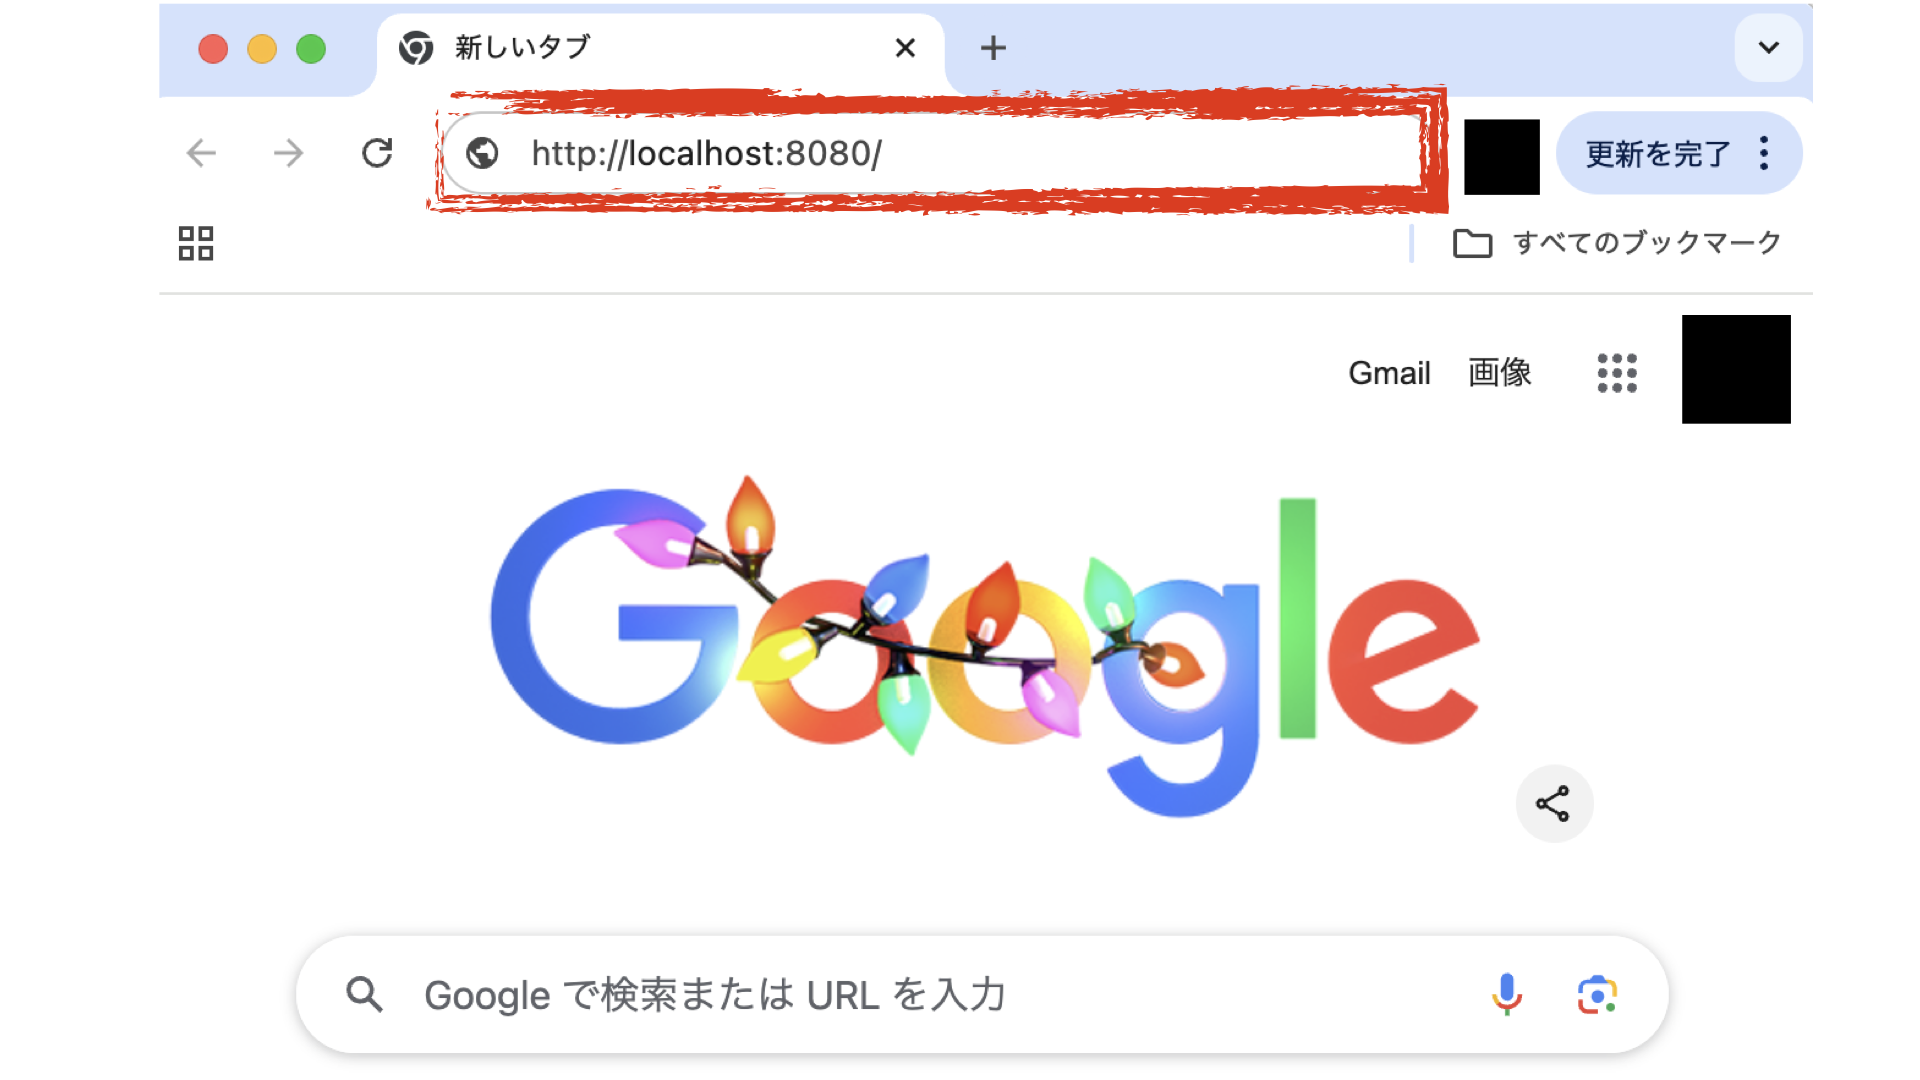
\includegraphics[width=13cm]{fig_web/URL.png}
  \caption{Google Chromeの場合のアドレスバーの位置}
  \label{fig:URL}
 \end{center}
\end{figure}
\begin{figure}[H]
 \begin{center}
  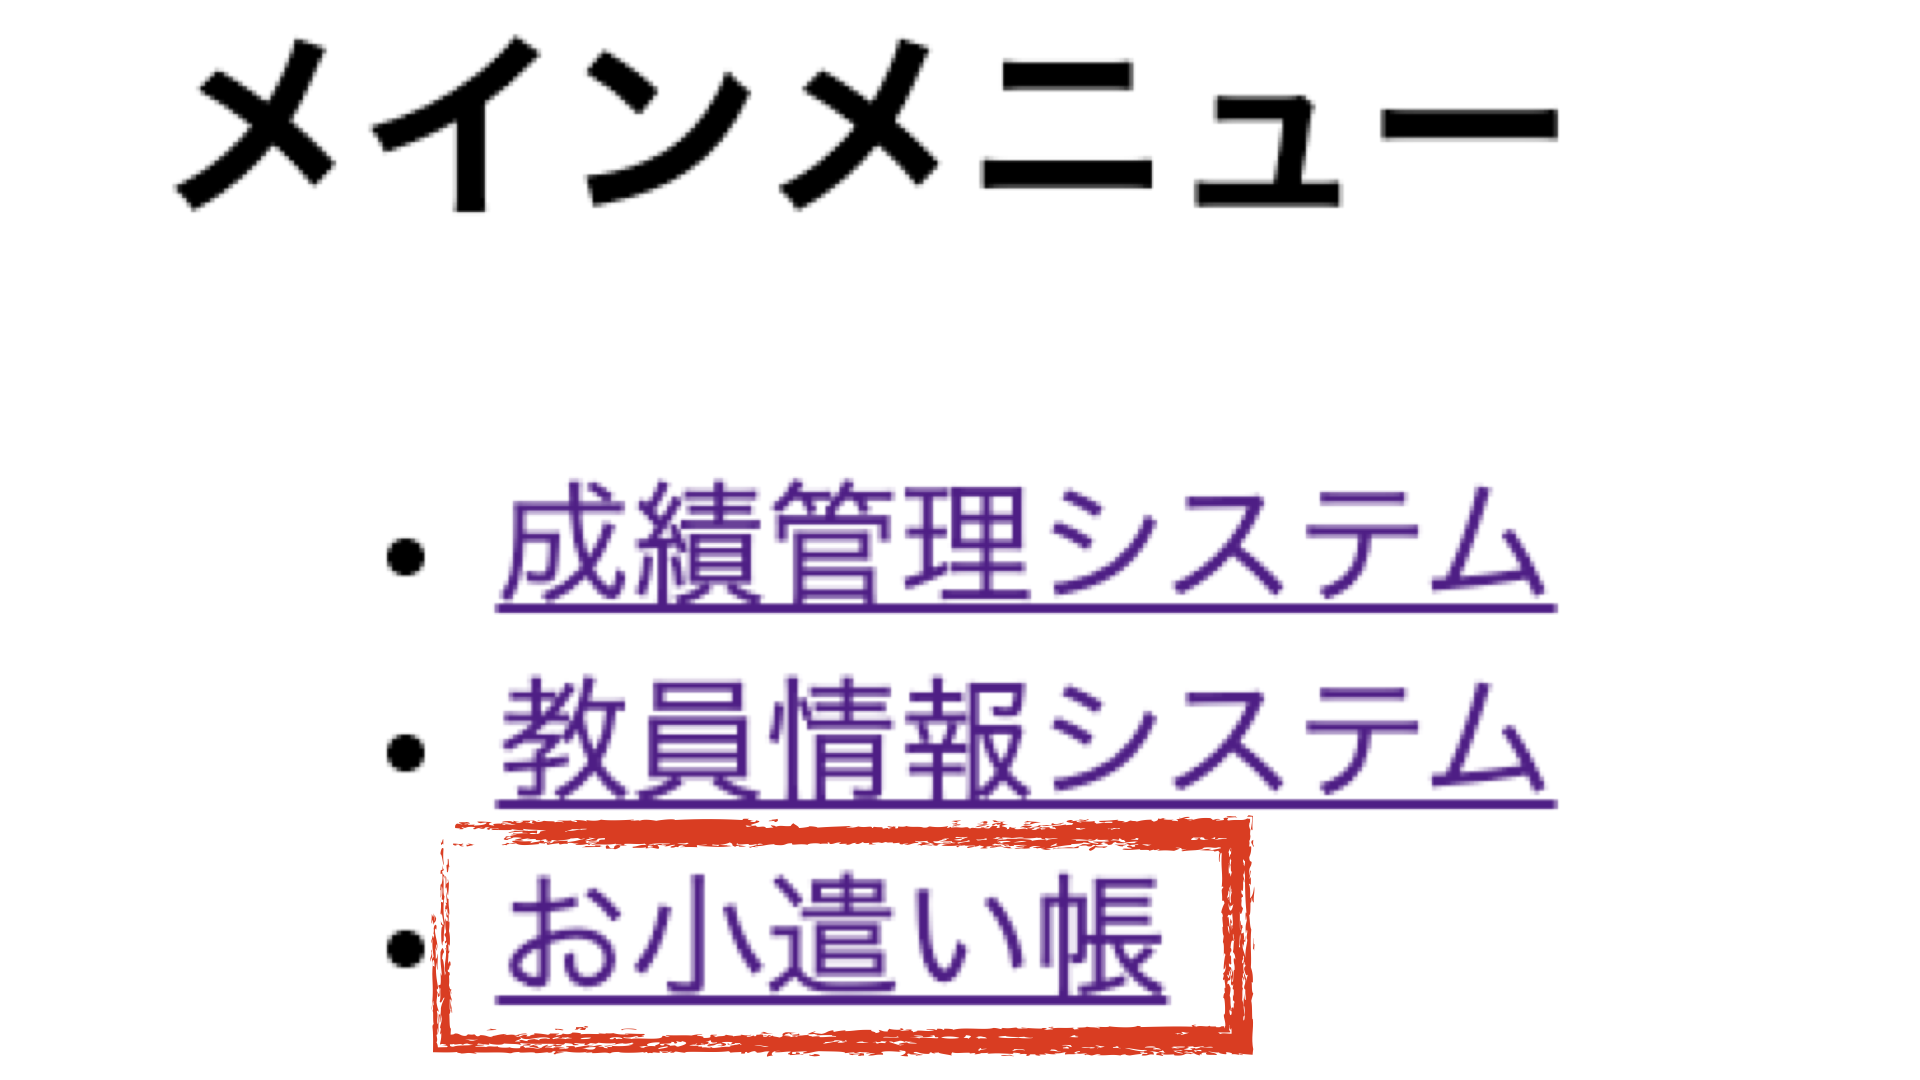
\includegraphics[width=5cm]{fig_web/top.png}
  \caption{メインメニュー画面}
  \label{fig:top}
 \end{center}
\end{figure}
\begin{figure}[H]
 \begin{center}
  
\includegraphics[width=5cm]{fig_web/404.png}
  \caption{存在しないページへアクセスした場合の画面}
  \label{fig:404}
 \end{center}
\end{figure}

\subsection{一覧表示}
お小遣い帳システムにアクセスすると，現在登録されているデータの一覧が表示される（図\ref{fig:list}）．
表には「日付」「項目」「値段」が表示され，表の最下部には登録されている全データの合計金額が自動計算されて表示される．
各項目のリンクをクリックすると，そのデータの詳細画面へ遷移する．

\begin{figure}[H]
 \begin{center}
  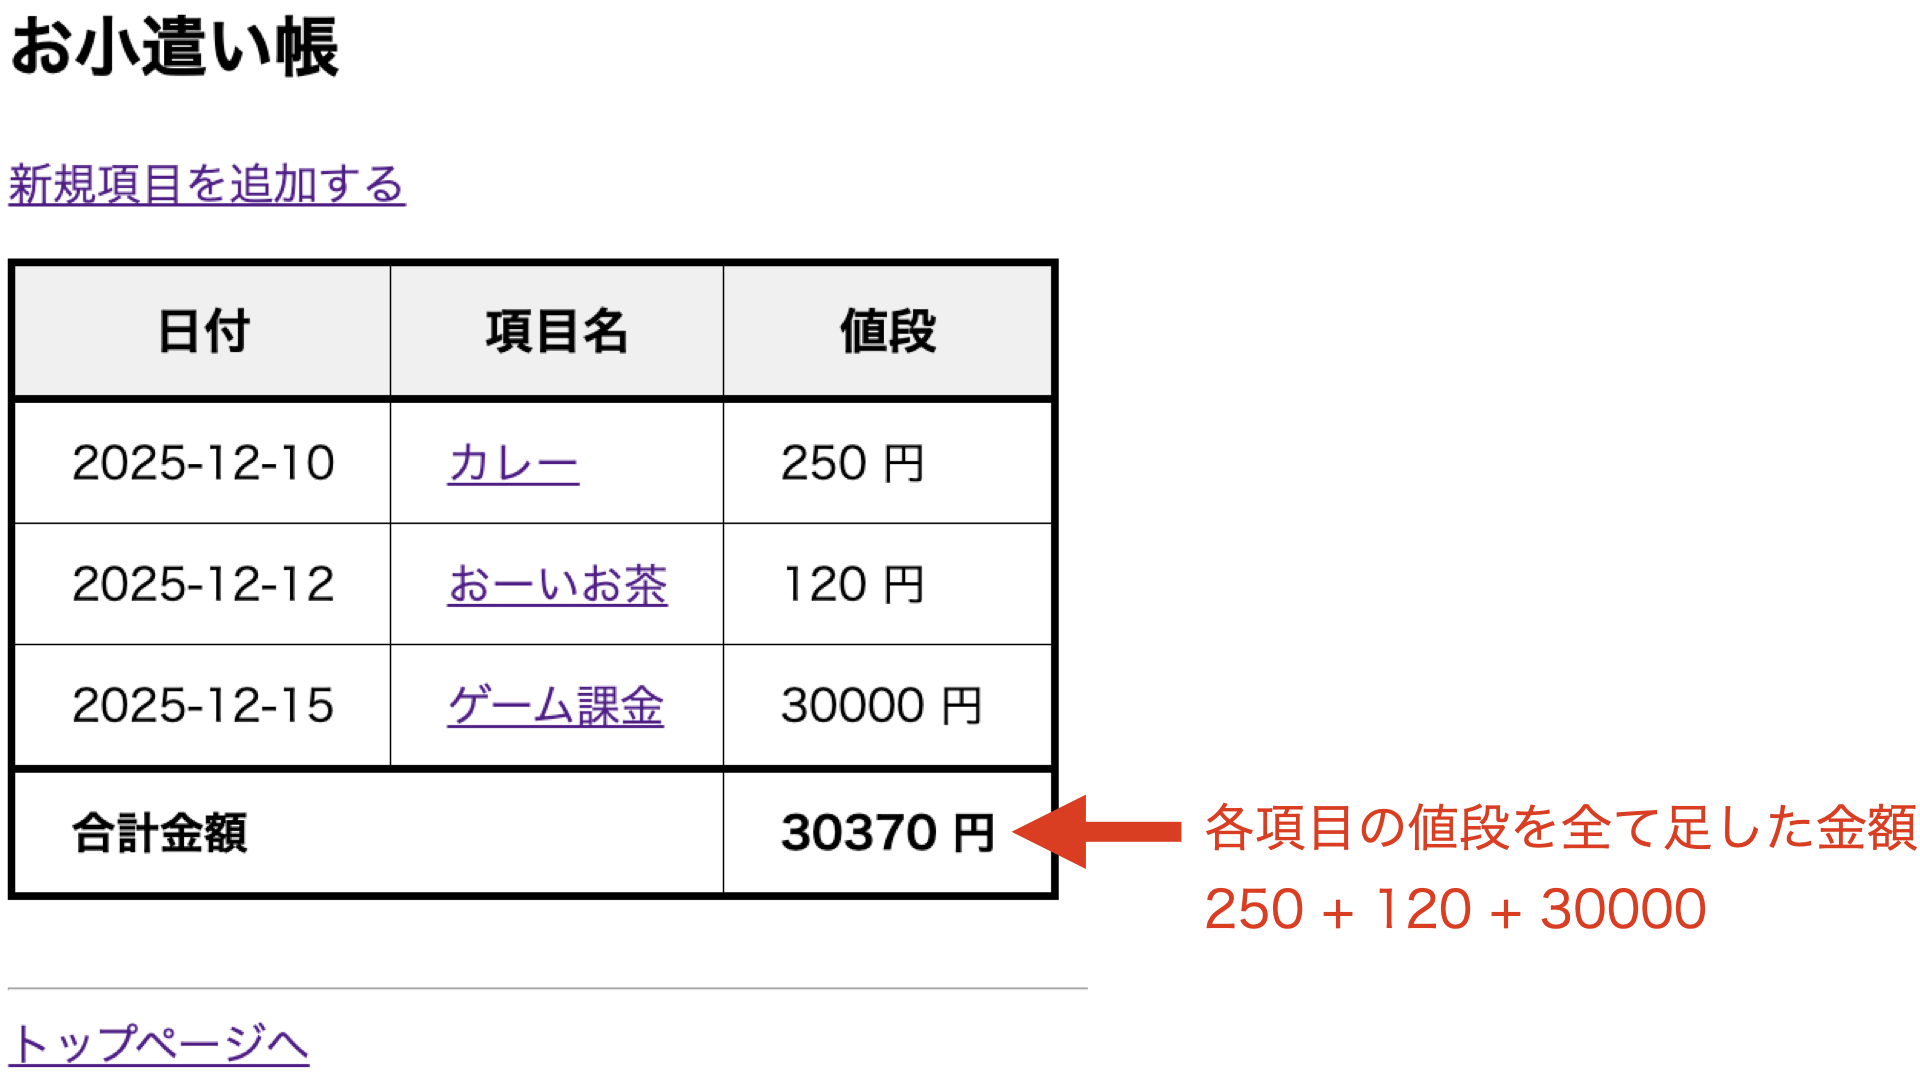
\includegraphics[width=13cm]{fig_web/wallet_list.png}
  \caption{お小遣い帳の一覧表示画面（合計金額が表示される）}
  \label{fig:list}
 \end{center}
\end{figure}

\subsection{詳細表示}
一覧画面で項目名をクリックすると，詳細表示画面へ遷移する（図\ref{fig:detail}）．
ここでは，一覧には表示しきれなかった「購入目的」や「備考欄」を含むすべての情報を確認できる．
また，この画面からデータの「編集」や「削除」を行うためのリンクが配置されている．

\begin{figure}[H]
 \begin{center}
  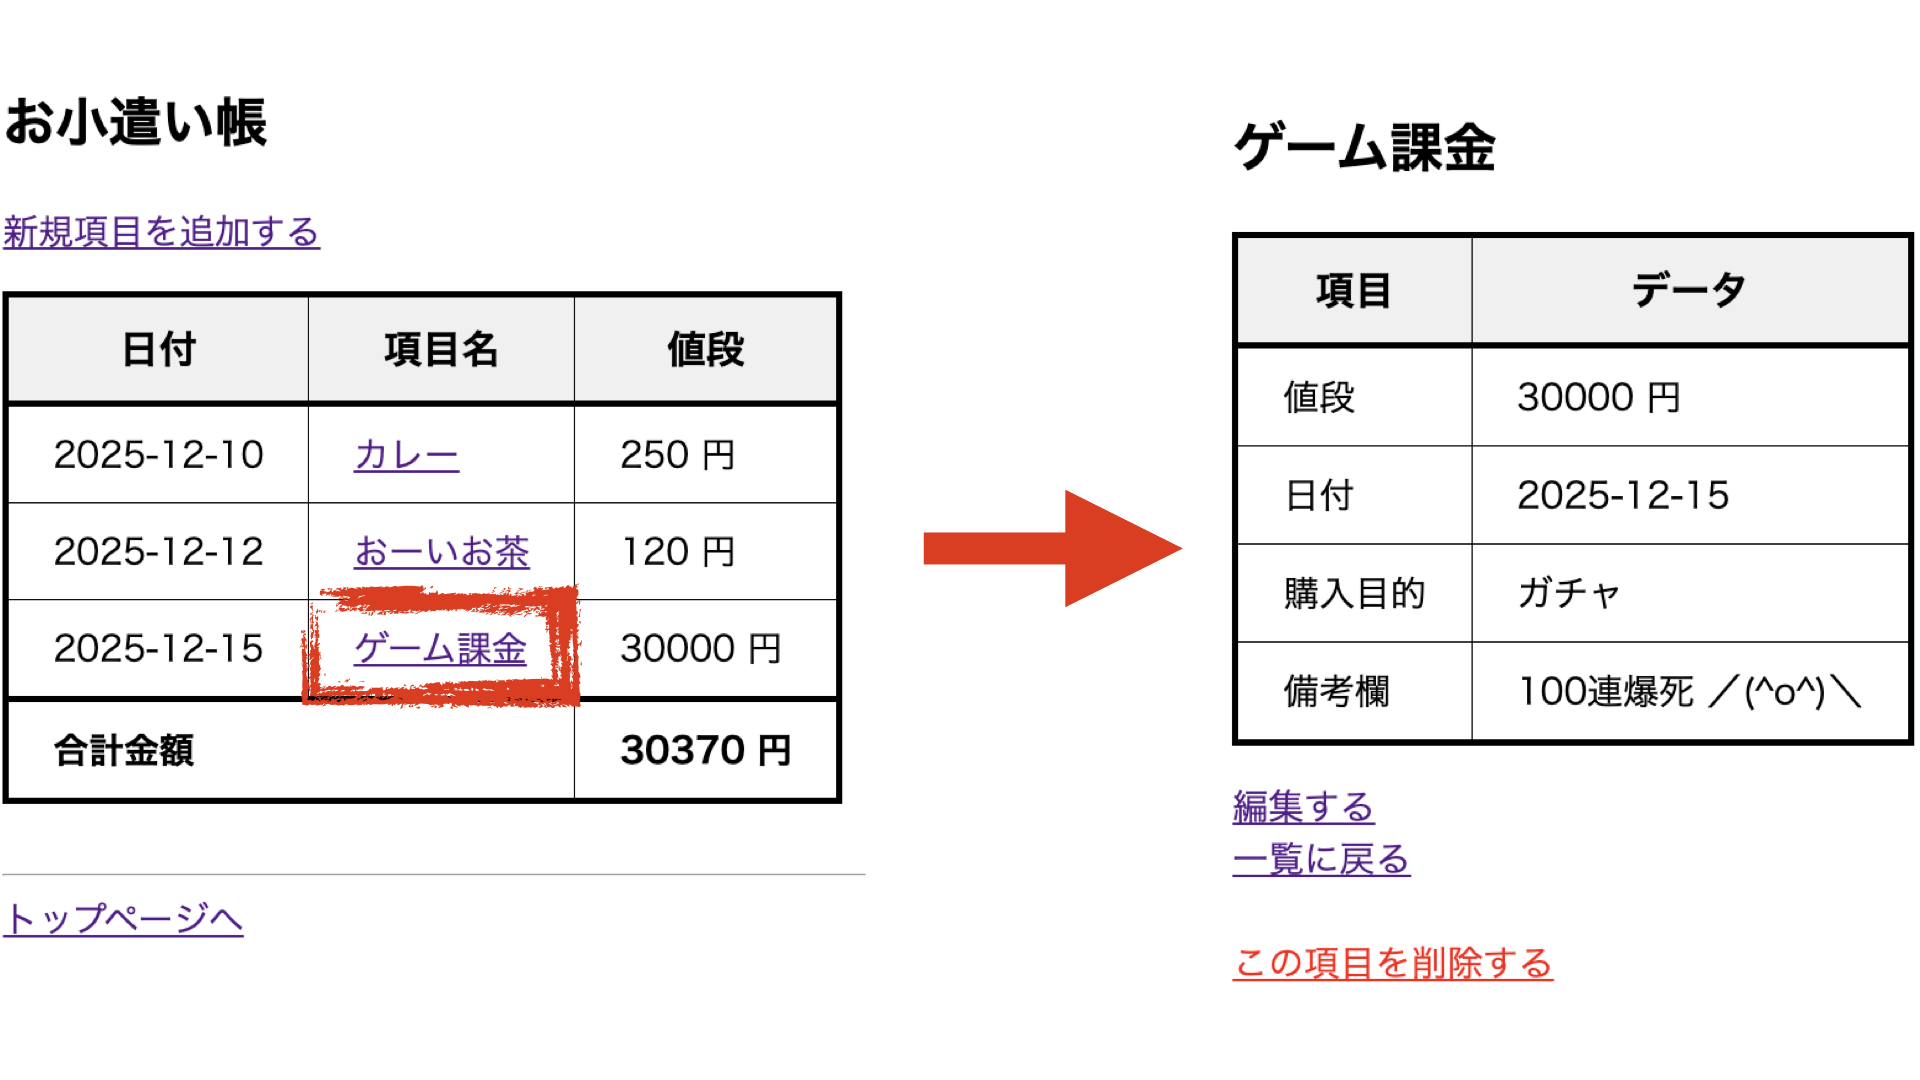
\includegraphics[width=15cm]{fig_web/wallet_detail.png}
  \caption{詳細表示の内容と仕方}
  \label{fig:detail}
 \end{center}
\end{figure}

\subsection{データの編集}
登録済みのデータを修正する手順は以下の通りである．
\begin{enumerate}
    \item 修正したいデータの詳細画面を開き，「編集する」リンクをクリックする（図\ref{fig:go_to_edit}）．
        \begin{figure}[H]
        \begin{center}
        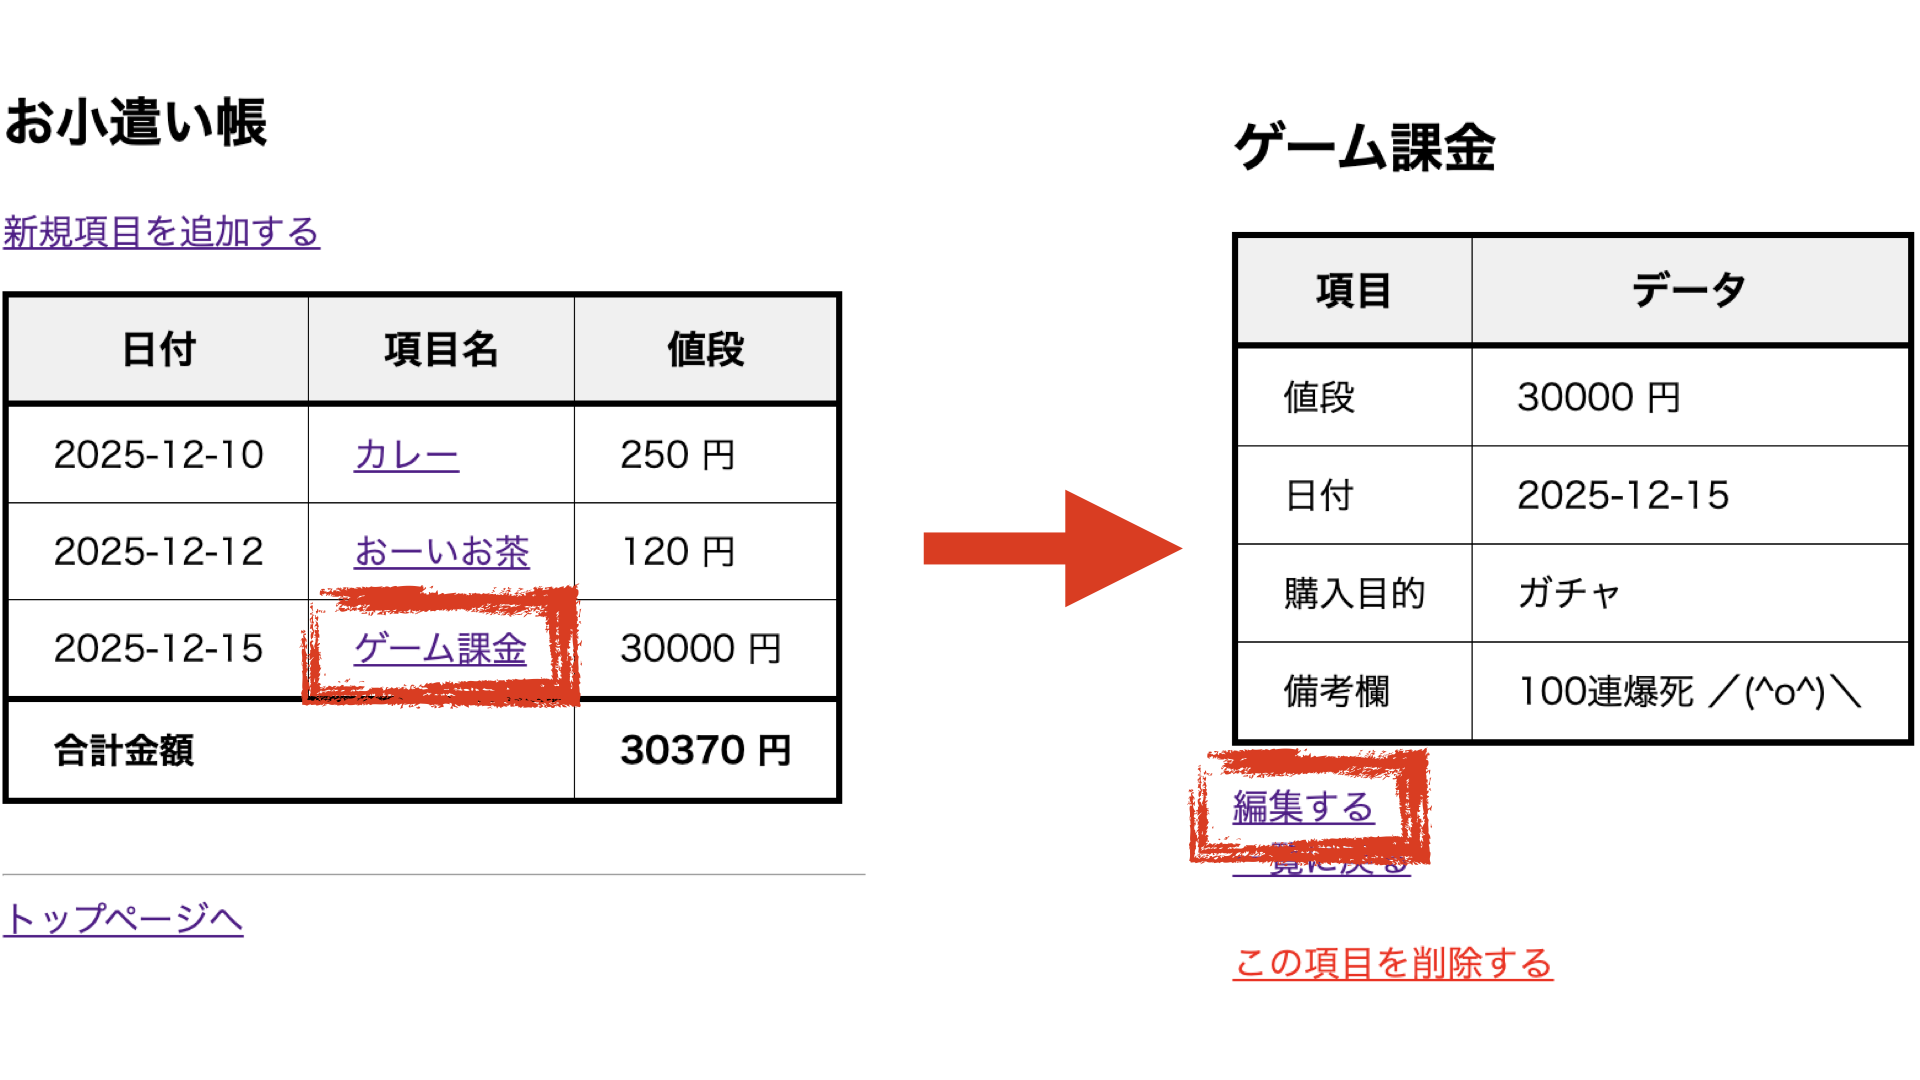
\includegraphics[width=15cm]{fig_web/wallet_go_to_edit.png}
        \caption{編集画面への行き方}
        \label{fig:go_to_edit}
        \end{center}
        \end{figure}
    \clearpage
    \item 編集画面が表示される（図\ref{fig:edit}）．現在のデータが入力欄に入った状態で表示されるため，修正したい箇所のみ書き換える．
        \begin{figure}[H]
        \begin{center}
        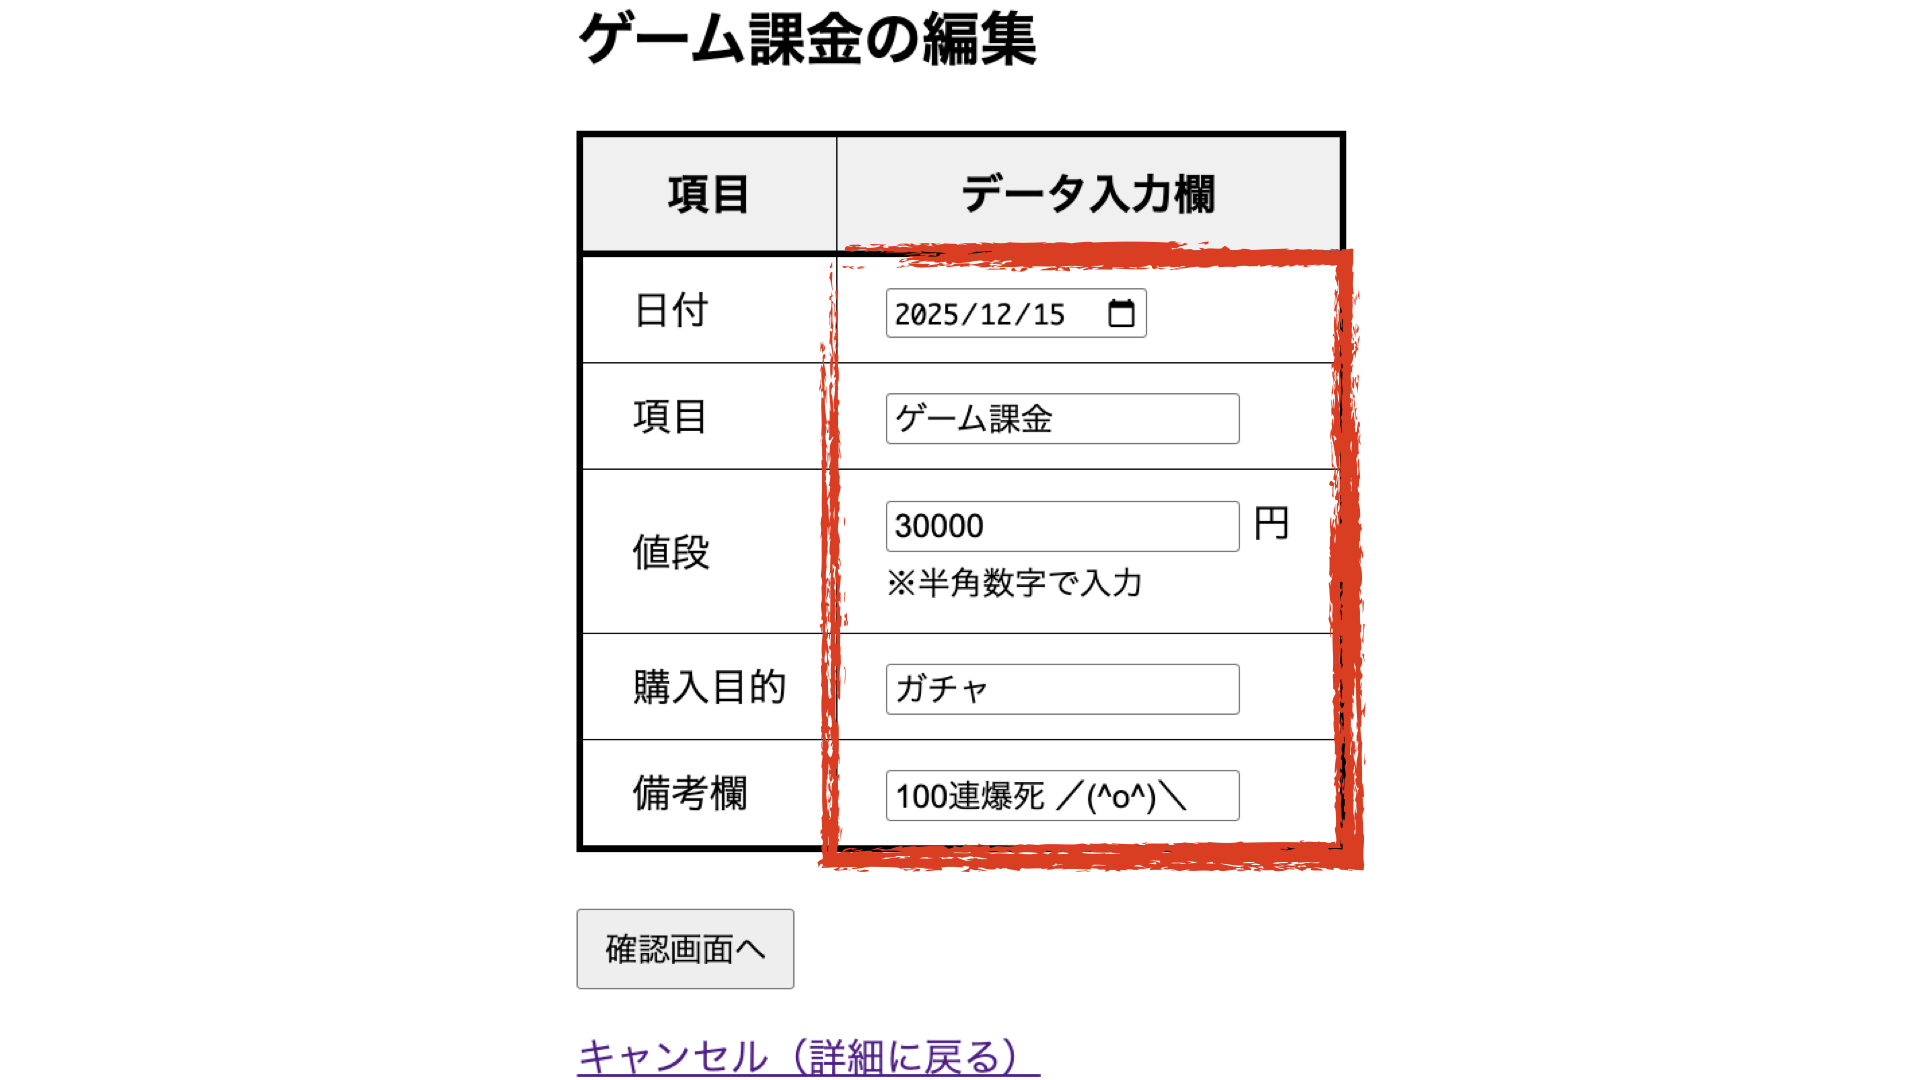
\includegraphics[width=15cm]{fig_web/wallet_edit.png}
        \caption{編集画面}
        \label{fig:edit}
        \end{center}
        \end{figure}
    \item 修正が完了したら「確認画面へ」ボタンを押す（図\ref{fig:edit_change}）．
        \begin{figure}[H]
        \begin{center}
        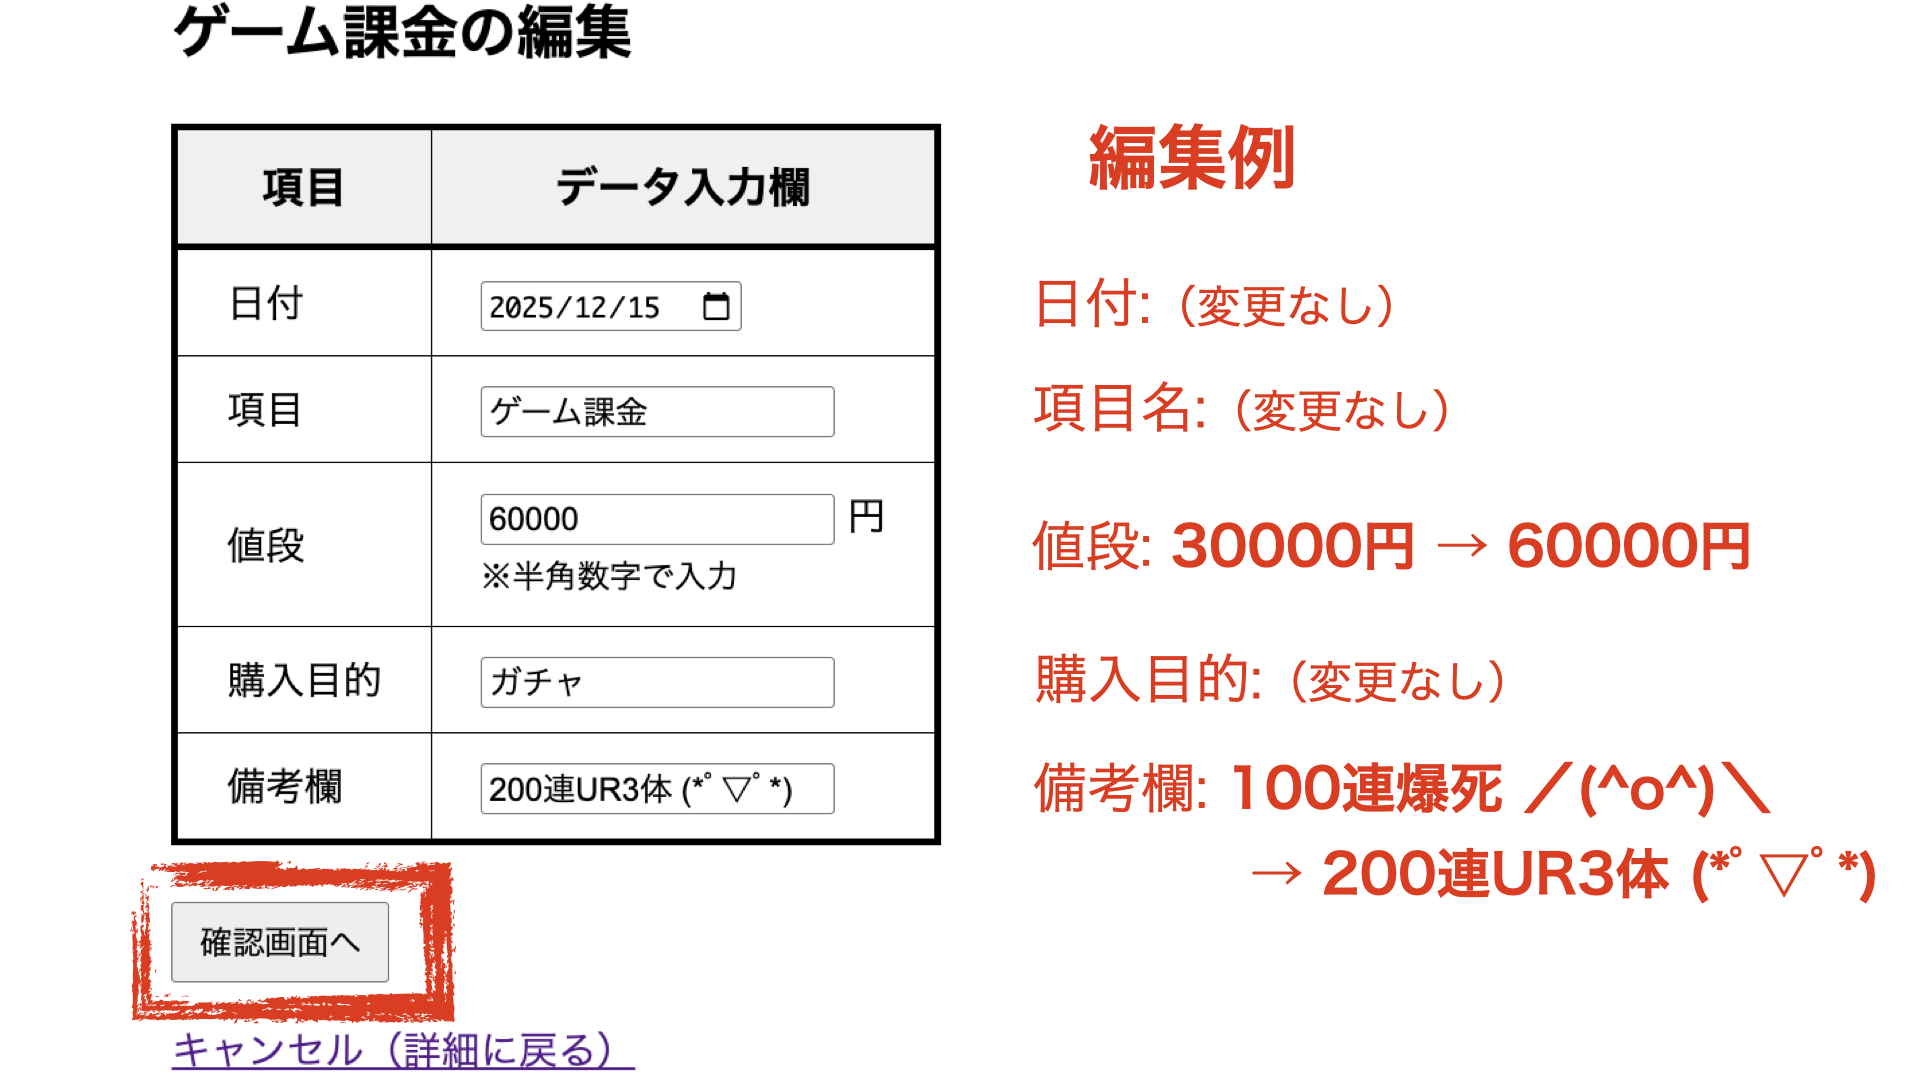
\includegraphics[width=15cm]{fig_web/wallet_edit_change.png}
        \caption{編集例と「確認画面へ」ボタン}
        \label{fig:edit_change}
        \end{center}
        \end{figure}
    \clearpage
    \item 表示された確認画面で変更内容を確認する（図\ref{fig:edit_confirm}）．修正が必要な場合は「修正する」ボタンを押して編集画面へ戻る．
        \begin{figure}[H]
        \begin{center}
        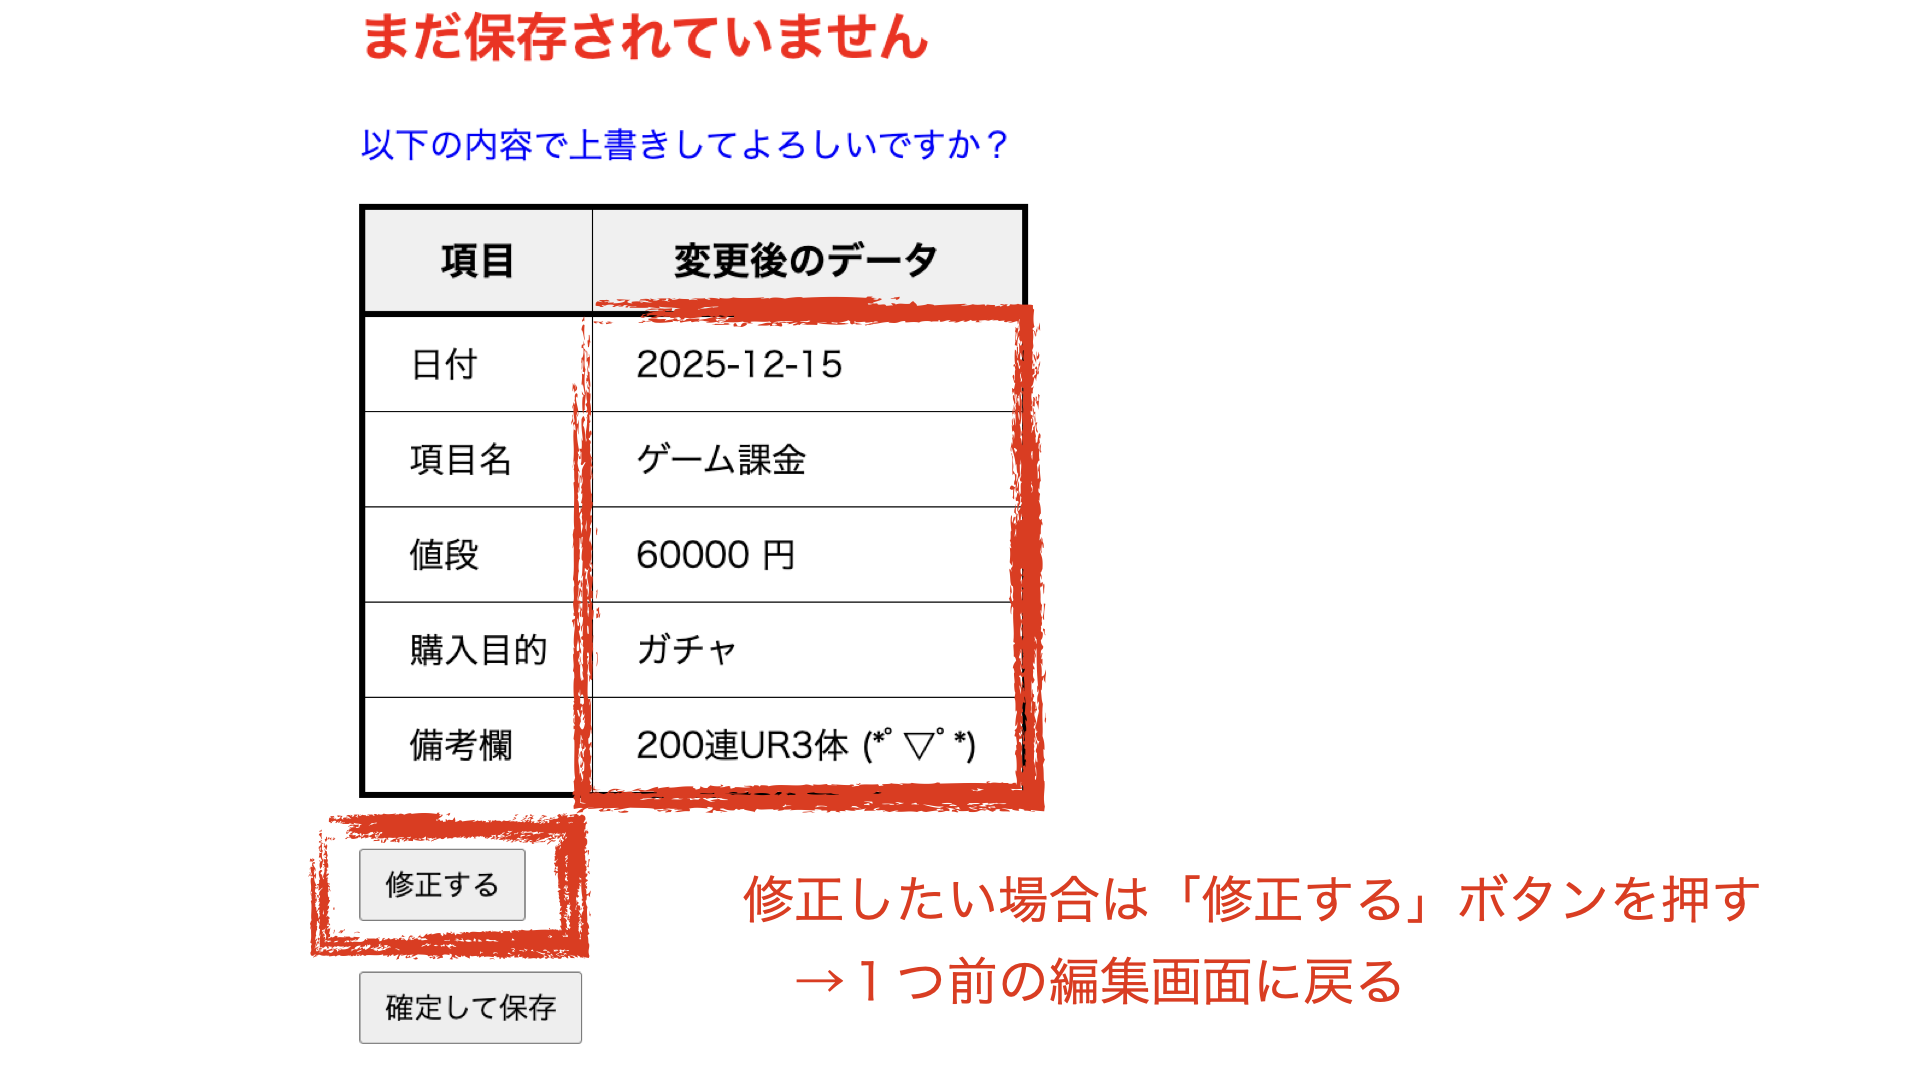
\includegraphics[width=15cm]{fig_web/wallet_edit_confirm.png}
        \caption{編集内容確認画面}
        \label{fig:edit_confirm}
        \end{center}
        \end{figure}
    \item 「確定して保存」ボタンを押すと，データが上書き保存され，詳細画面へ戻る（図\ref{fig:edit_fin1}）．一覧表示にも変更が反映されている（図\ref{fig:edit_fin2}）．
        \begin{figure}[H]
        \begin{center}
        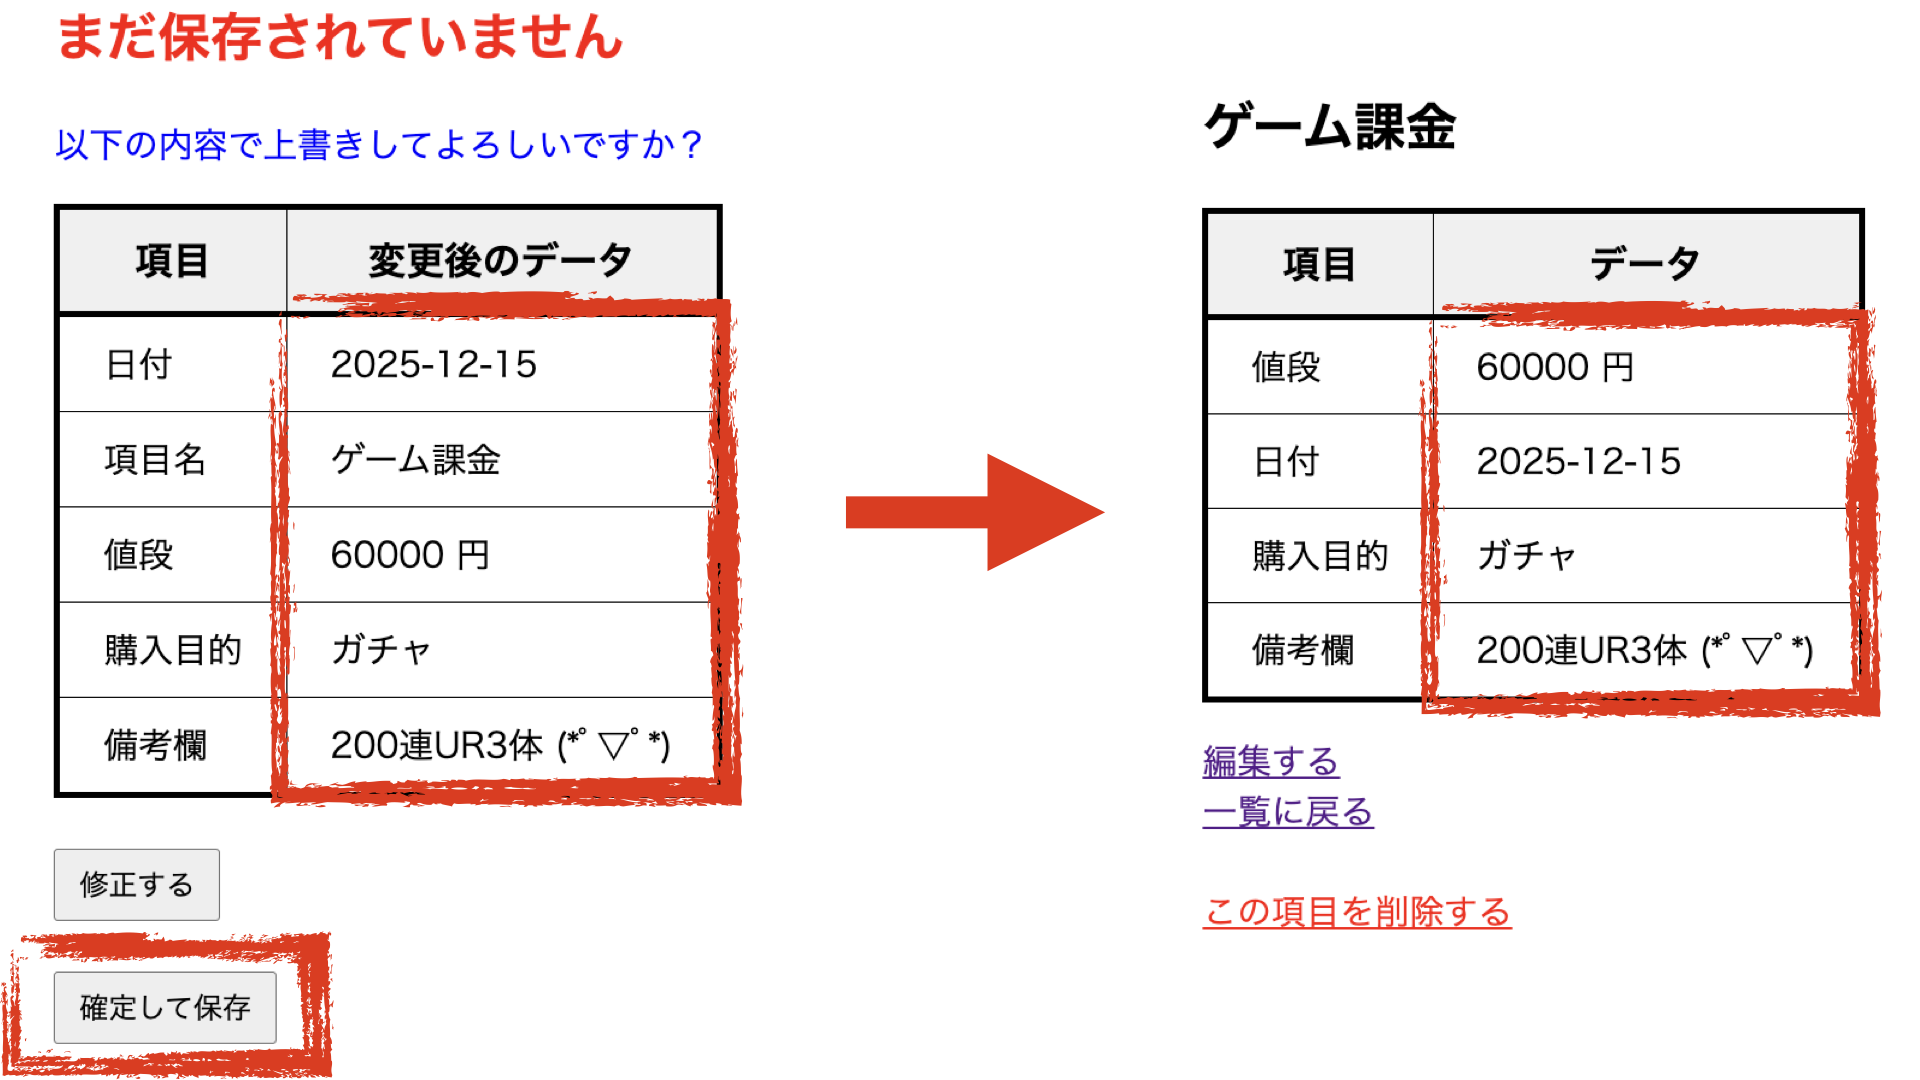
\includegraphics[width=15cm]{fig_web/wallet_edit_fin1.png}
        \caption{編集完了後の画面}
        \label{fig:edit_fin1}
        \end{center}
        \end{figure}
        \begin{figure}[H]
        \begin{center}
        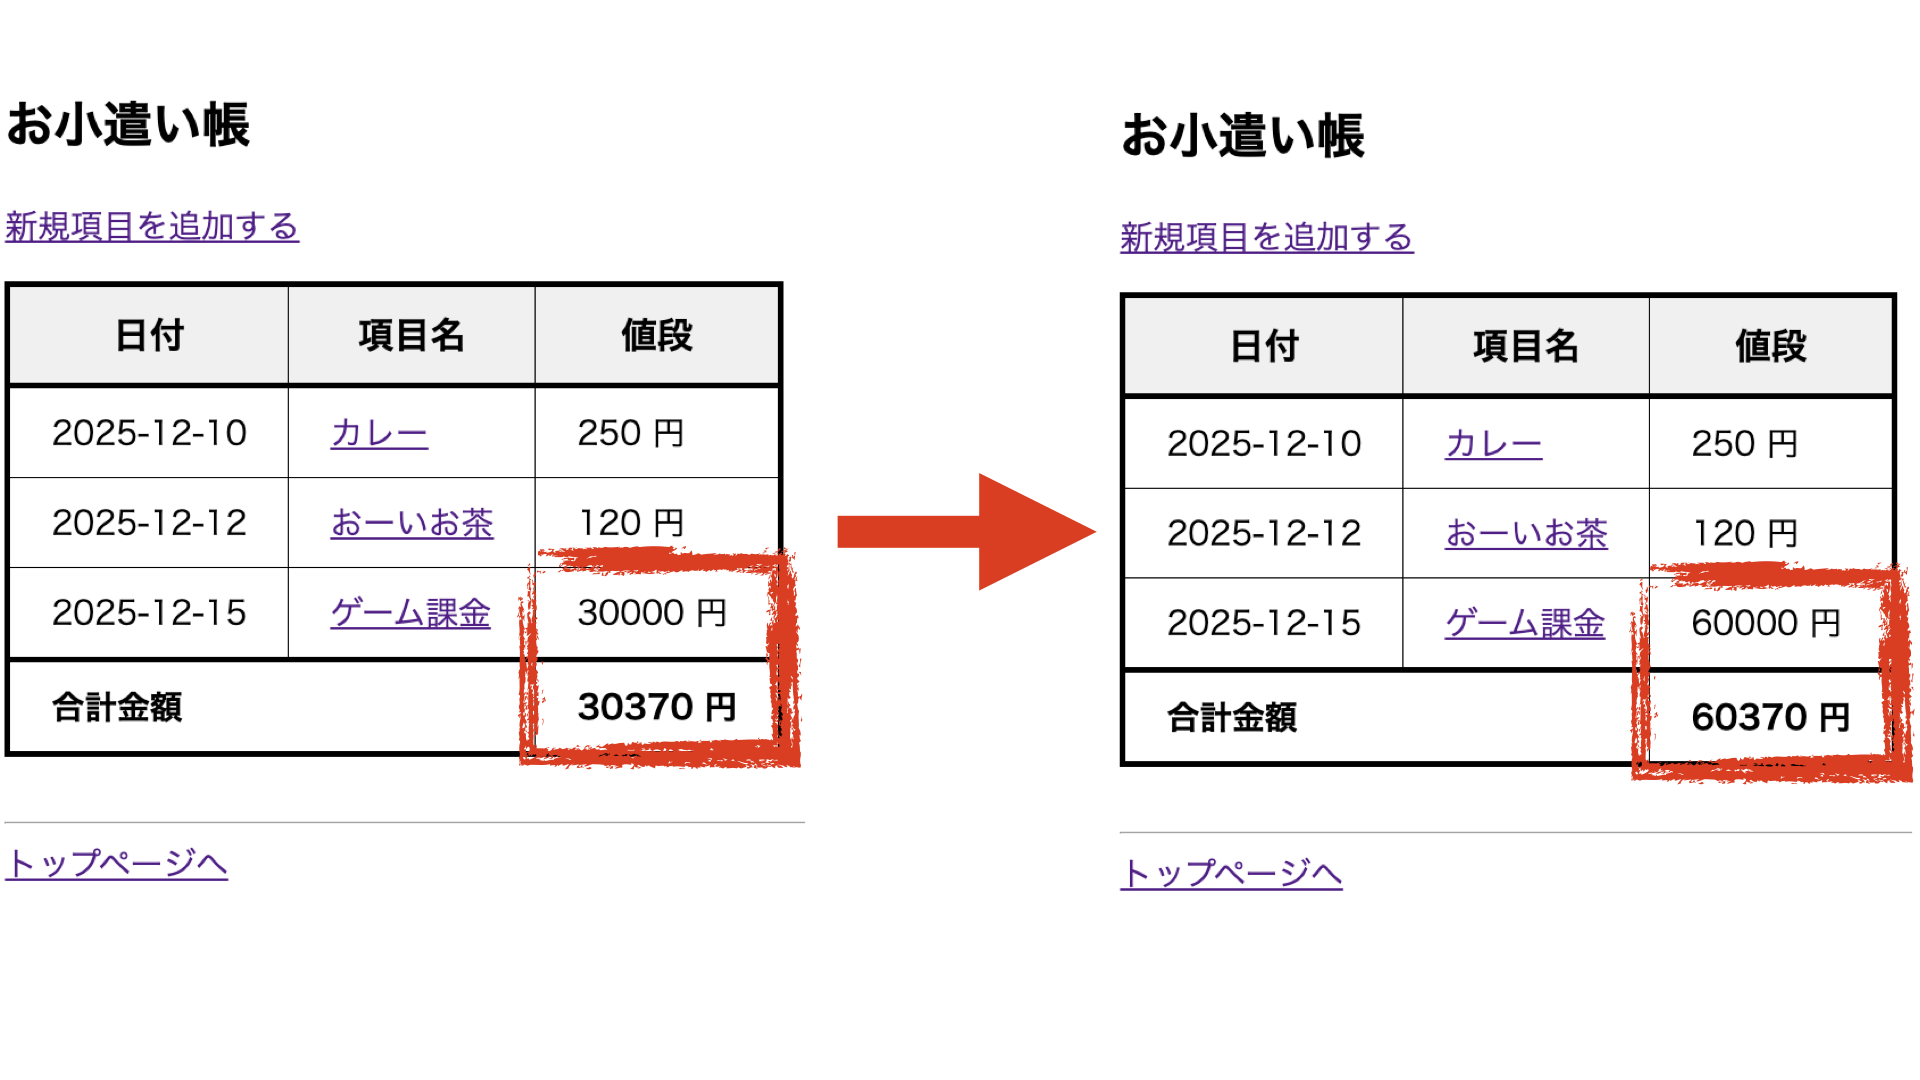
\includegraphics[width=15cm]{fig_web/wallet_edit_fin2.png}
        \caption{編集前と後の一覧表示画面}
        \label{fig:edit_fin2}
        \end{center}
        \end{figure}
\end{enumerate}

\subsection{データの追加}
新しいデータを登録する手順は以下の通りである．
\begin{enumerate}
    \item 一覧表示画面の上方にある「新規項目を追加する」リンクをクリックする（図\ref{fig:go_to_add}）．
        \begin{figure}[H]
        \begin{center}
        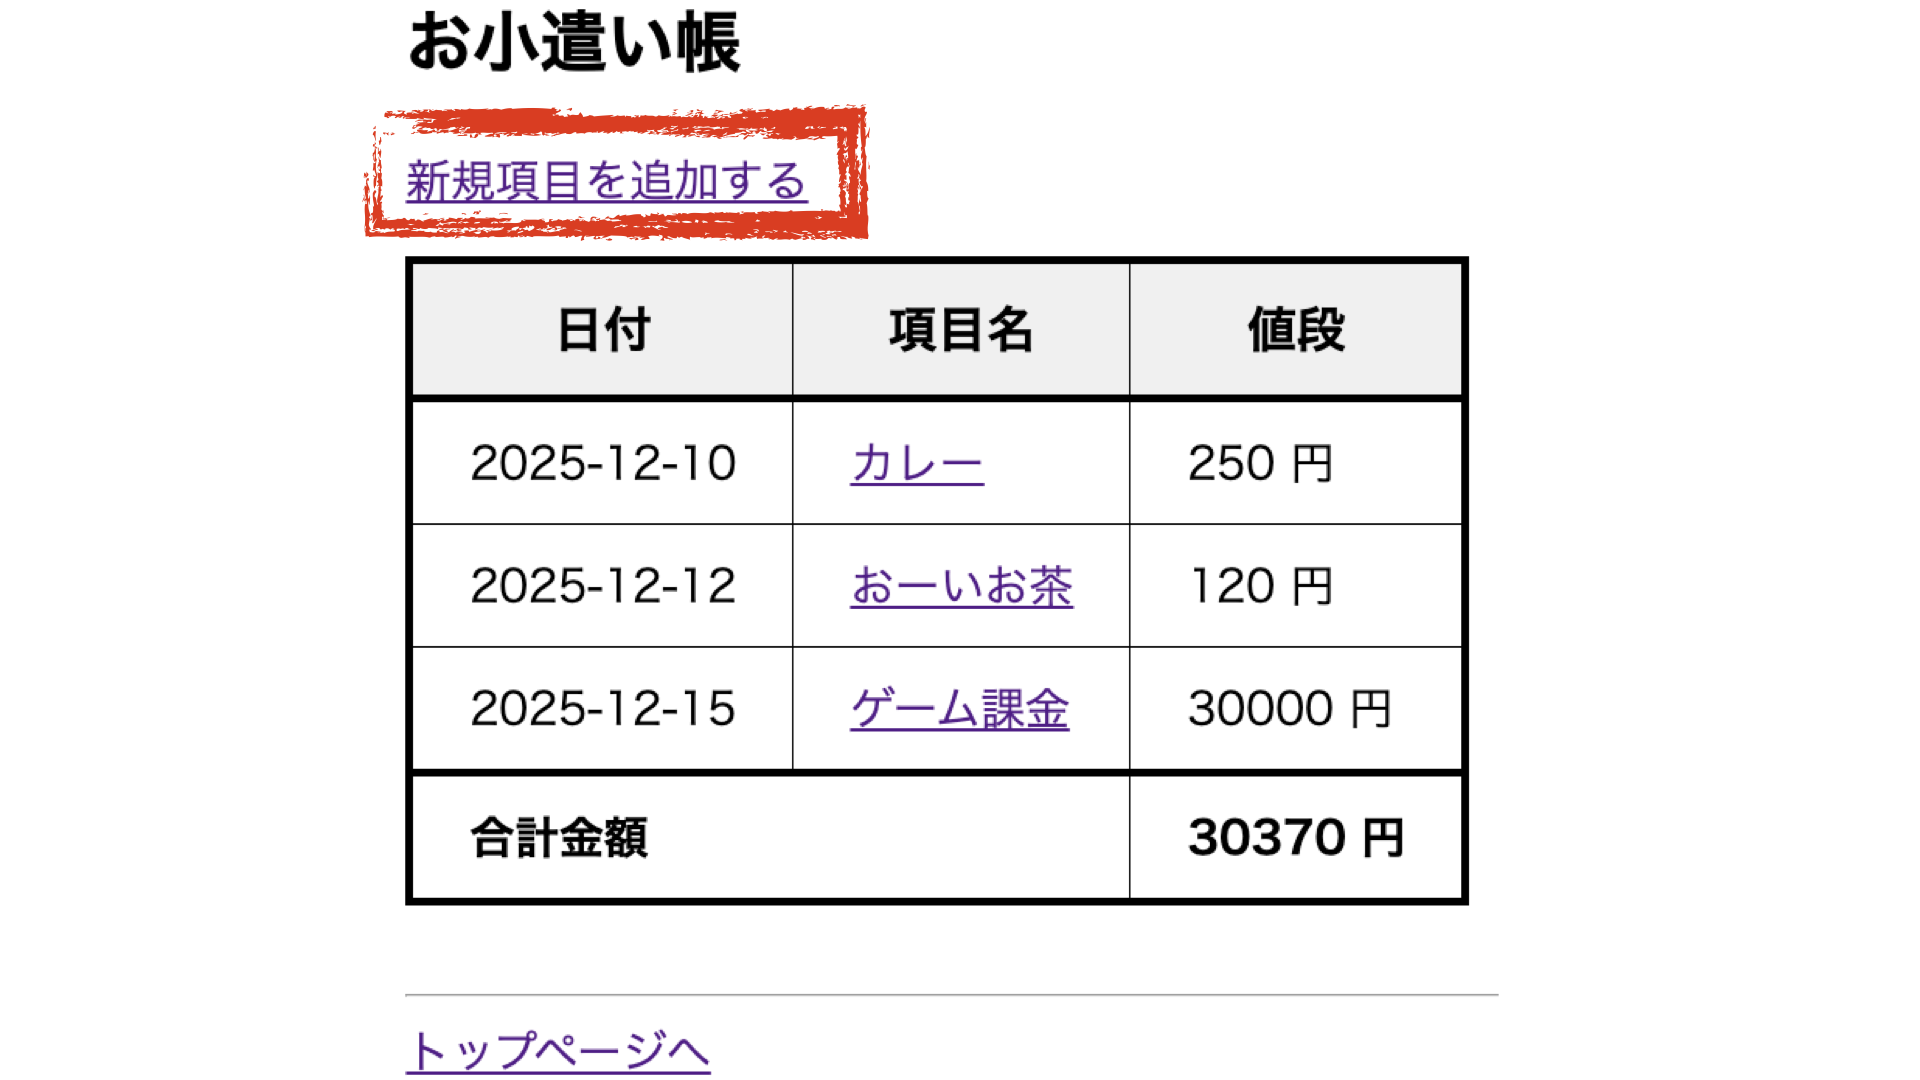
\includegraphics[width=15cm]{fig_web/wallet_go_to_add.png}
        \caption{新規登録画面への行き方}
        \label{fig:go_to_add}
        \end{center}
        \end{figure}
    \item 新規登録画面が表示される（図\ref{fig:add}）．日付，項目名，値段（半角数字），購入目的，備考欄を入力する．
        \begin{figure}[H]
        \begin{center}
        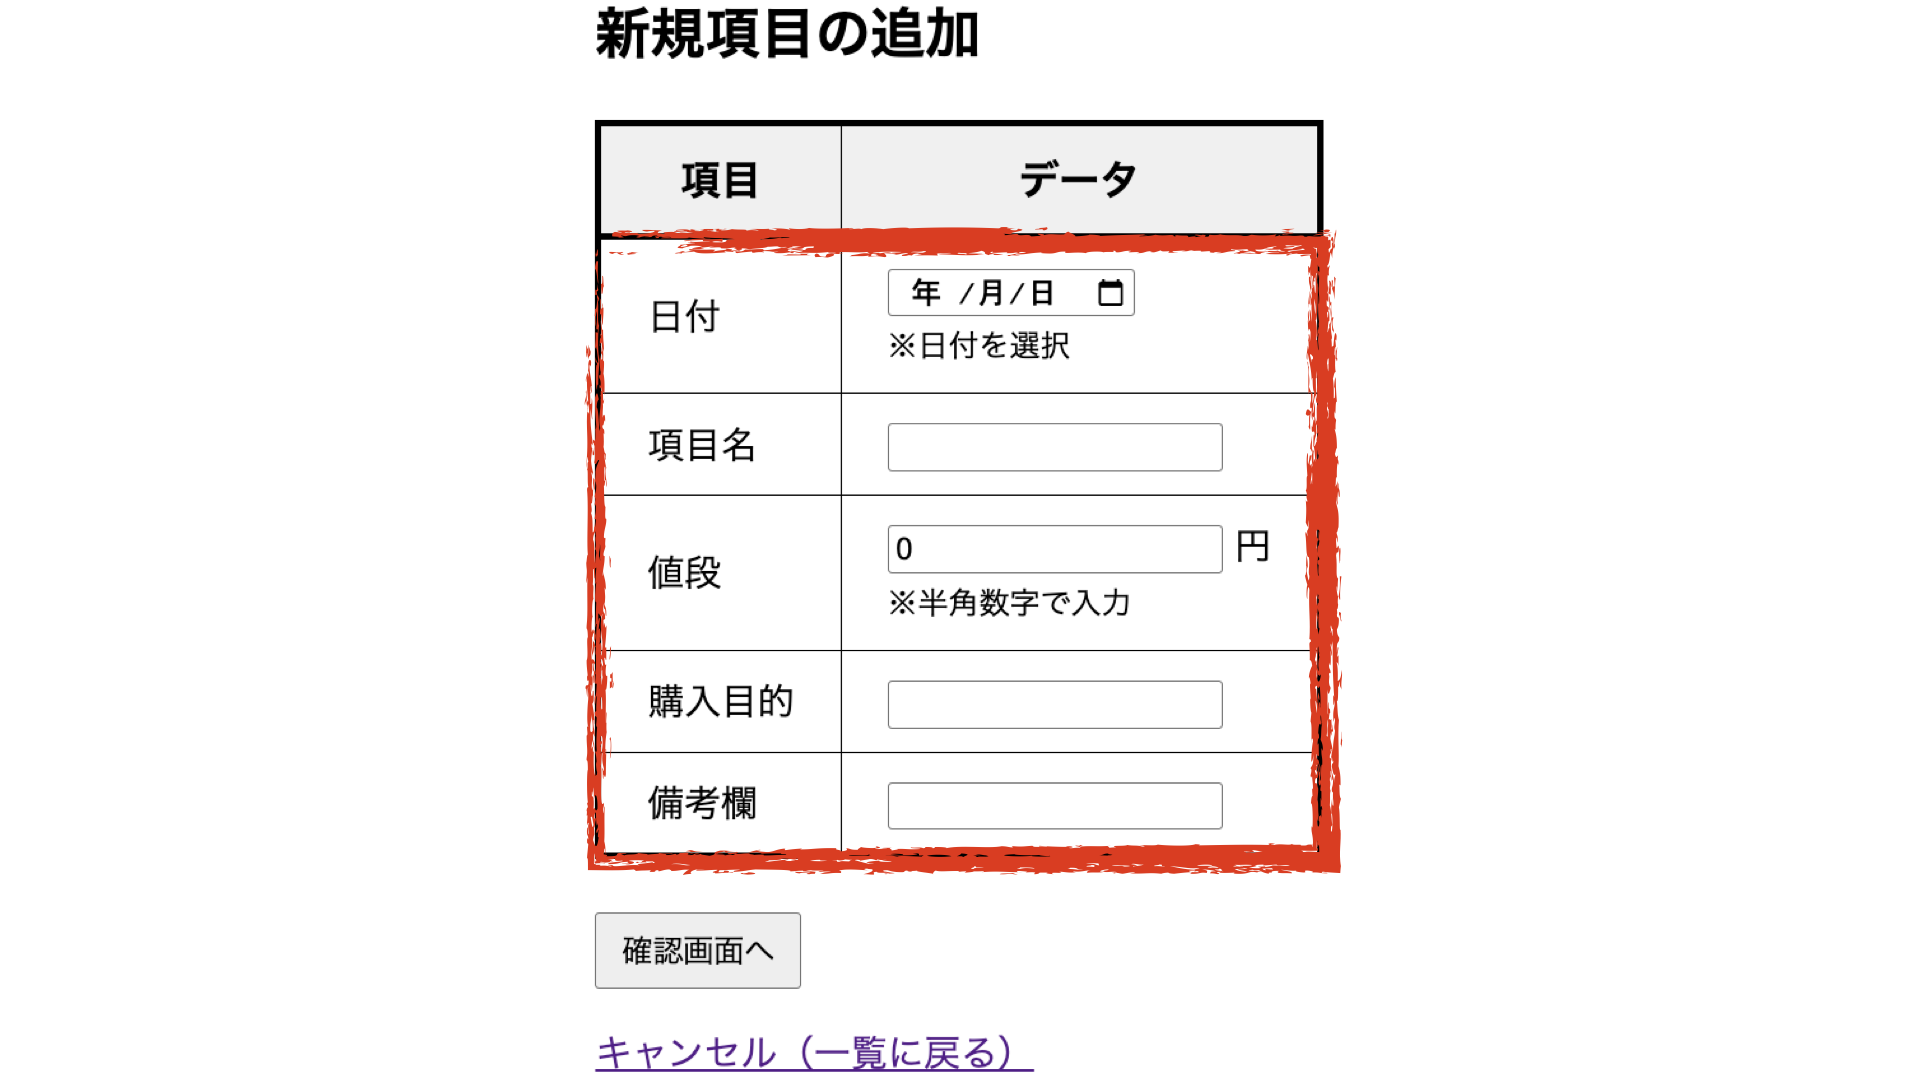
\includegraphics[width=15cm]{fig_web/wallet_add.png}
        \caption{新規登録画面}
        \label{fig:add}
        \end{center}
        \end{figure}
    \item 入力が完了したら「確認画面へ」ボタンを押す（図\ref{fig:add_change}）．
        \begin{figure}[H]
        \begin{center}
        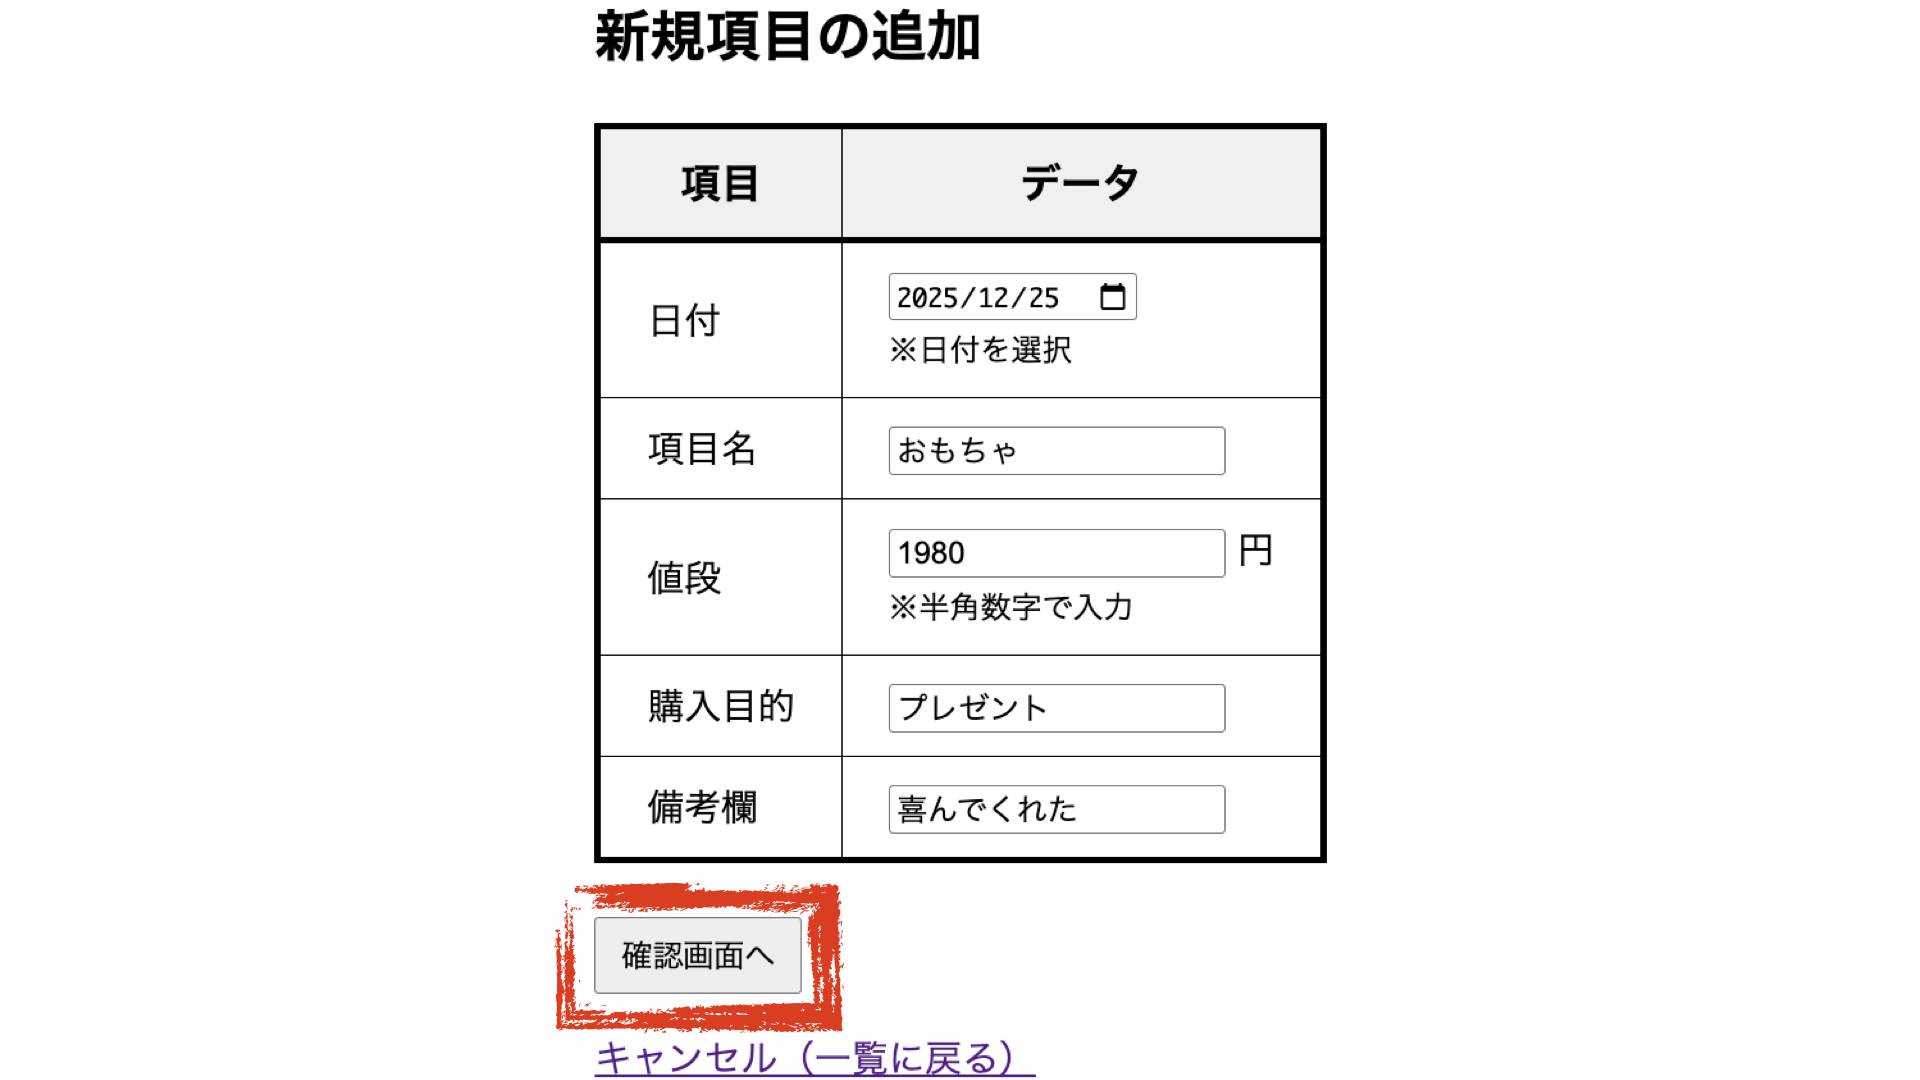
\includegraphics[width=15cm]{fig_web/wallet_add_change.png}
        \caption{新規登録入力例と「確認画面へ」ボタン}
        \label{fig:add_change}
        \end{center}
        \end{figure}
    \item 新規登録内容の確認画面が表示される（図\ref{fig:add_confirm}）．内容に間違いがなければ「追加する」ボタンを押す．修正が必要な場合は「修正する」ボタンを押して入力画面へ戻る．
        \begin{figure}[H]
        \begin{center}
        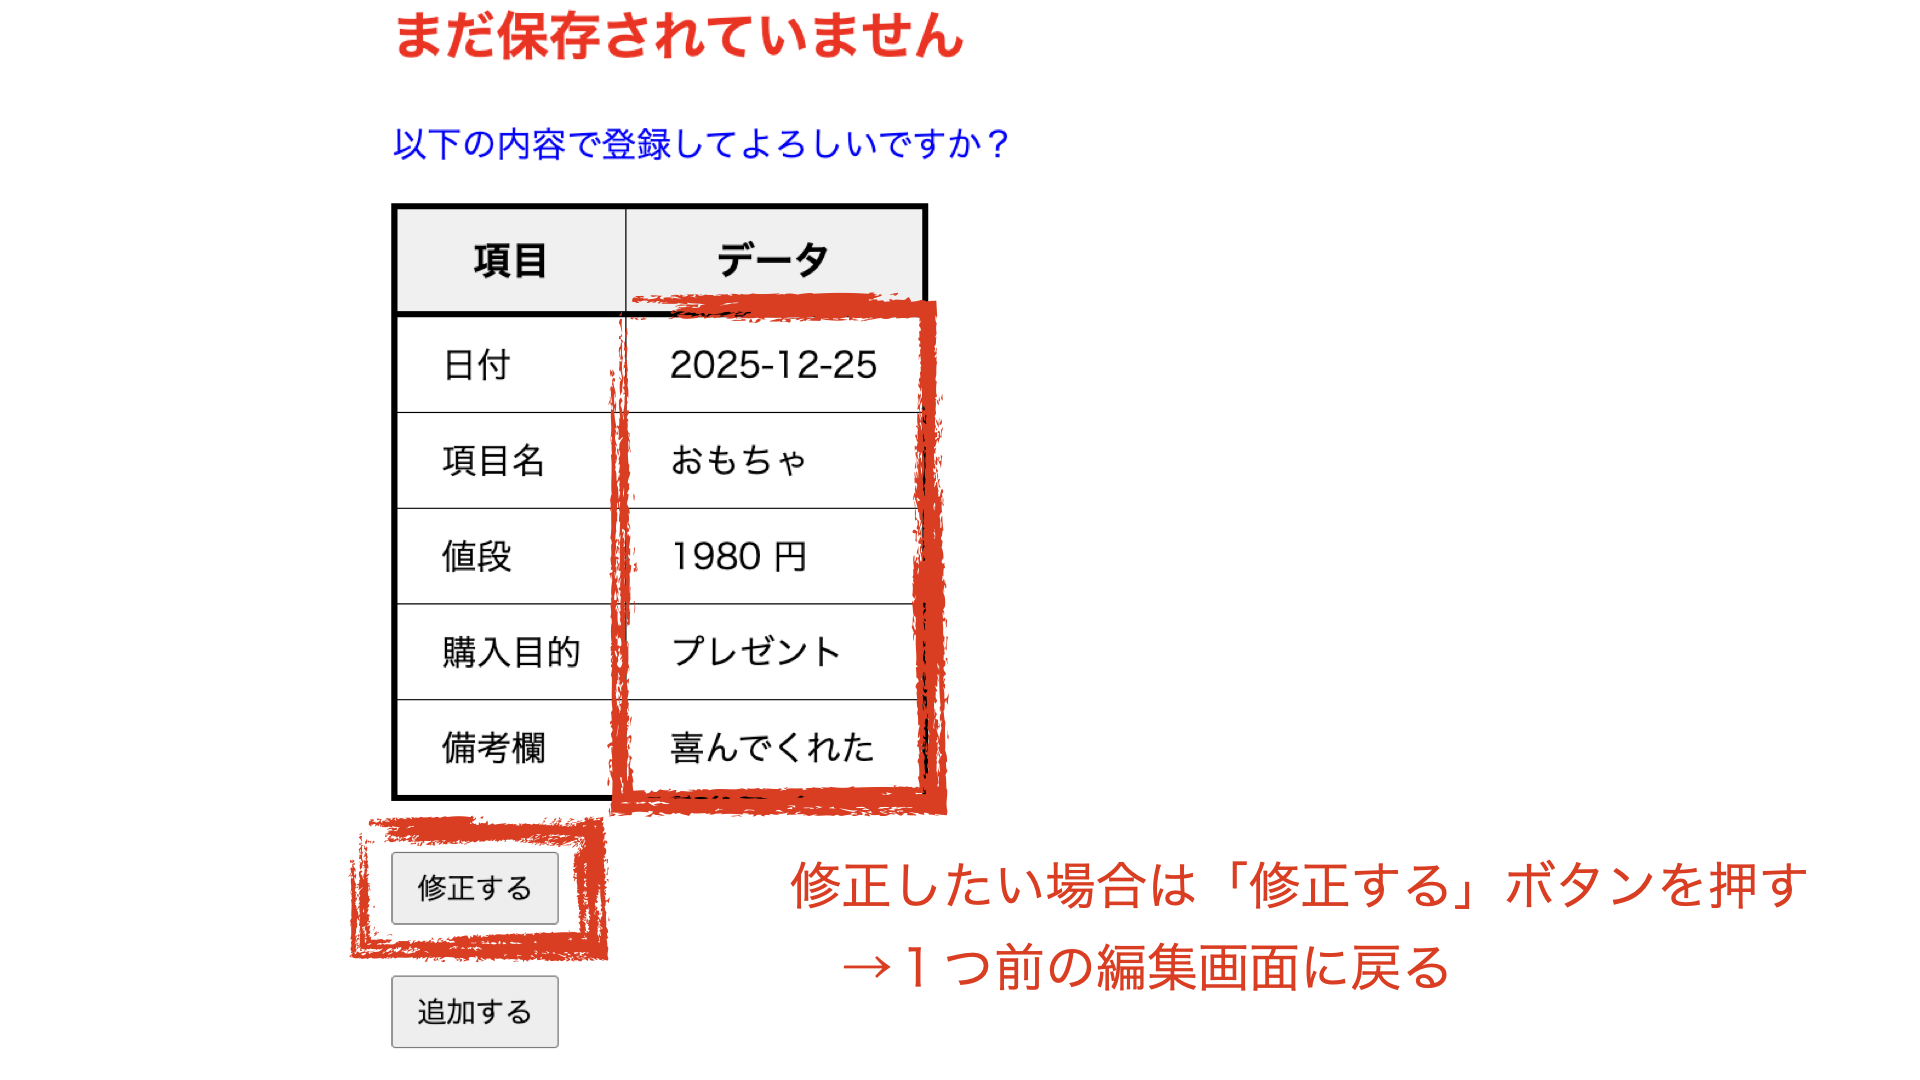
\includegraphics[width=15cm]{fig_web/wallet_add_confirm.png}
        \caption{新規登録内容確認画面}
        \label{fig:add_confirm}
        \end{center}
        \end{figure}
    \item 「追加する」を押すとデータが保存され，一覧表示画面に追加されたデータが表示される（図\ref{fig:add_fin1}）．
        \begin{figure}[H]
        \begin{center}
        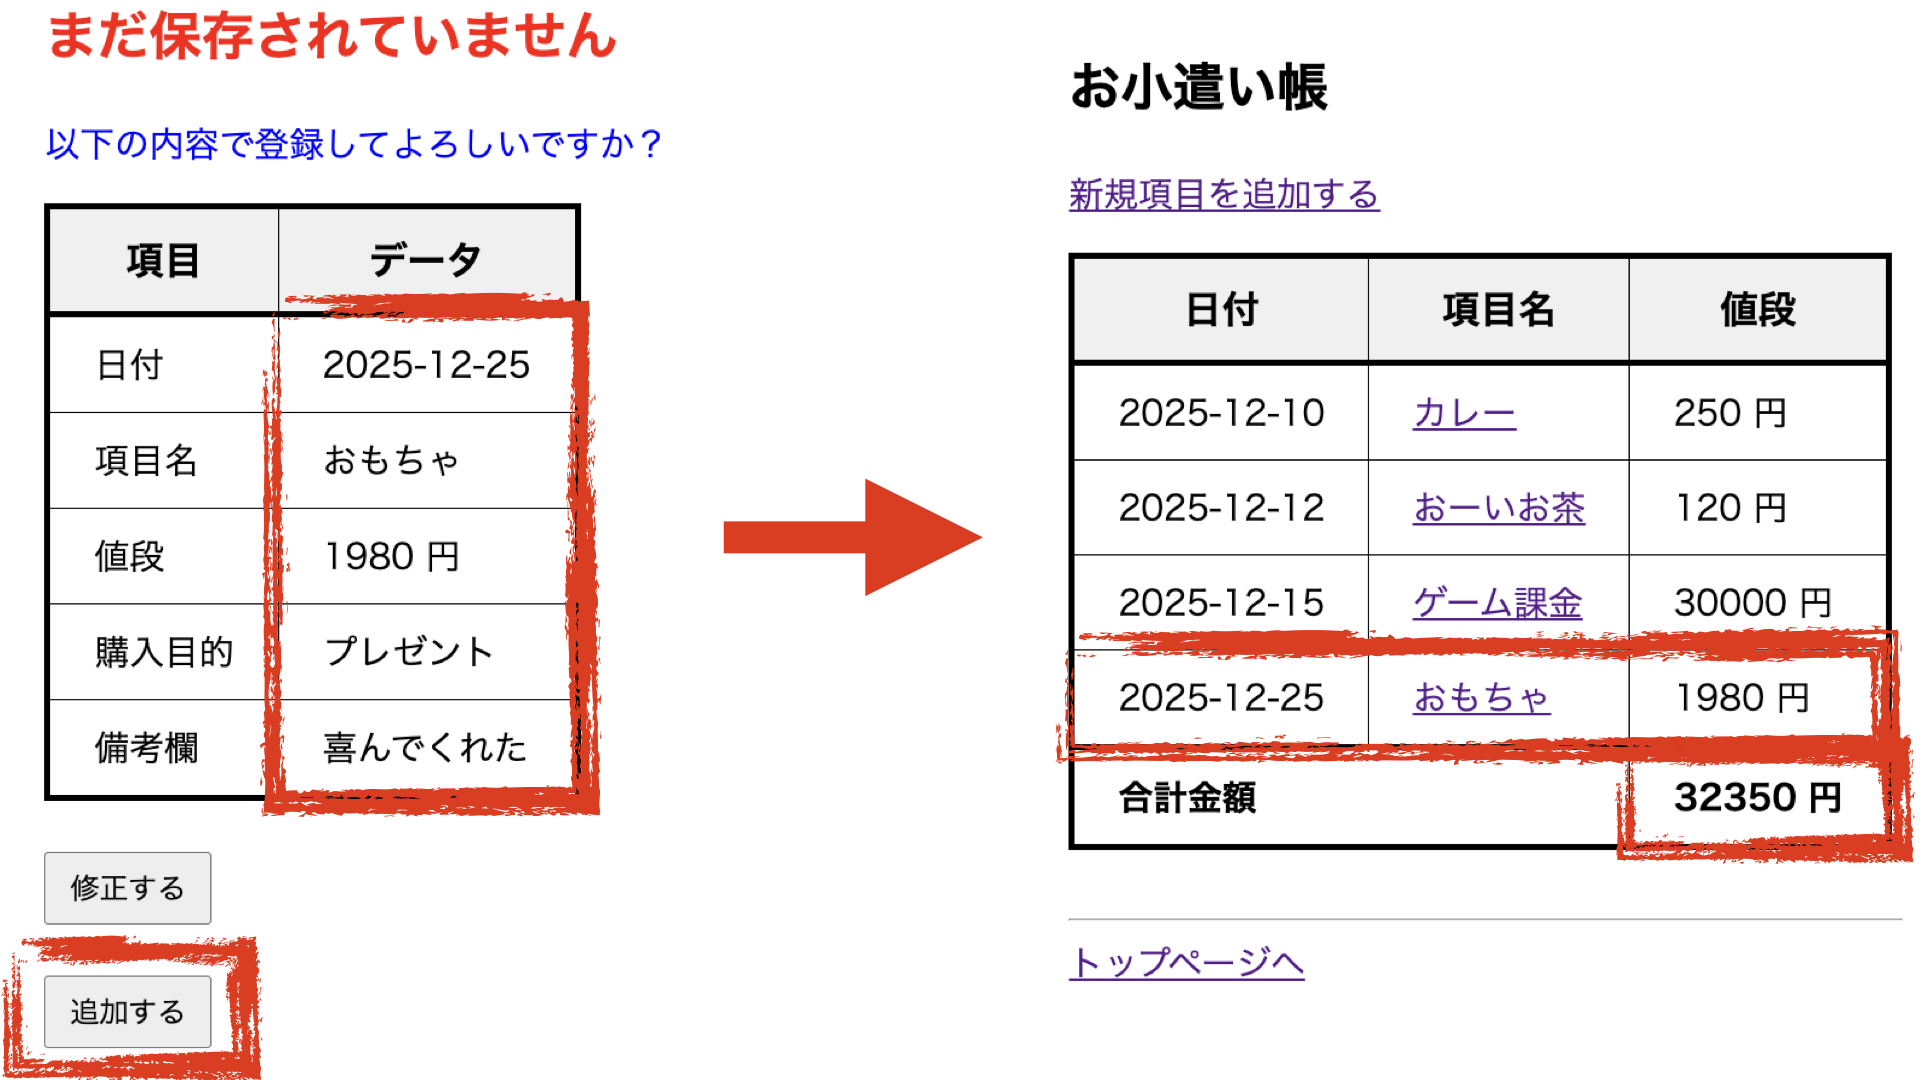
\includegraphics[width=15cm]{fig_web/wallet_add_fin.png}
        \caption{新規登録完了後の画面}
        \label{fig:add_fin1}
        \end{center}
        \end{figure}
\end{enumerate}

\subsection{データの削除}
不要になったデータを削除する手順は以下の通りである．
\begin{enumerate}
    \item 削除したいデータの詳細画面を開き，赤字で表示された「削除する」リンクをクリックする（図\ref{fig:go_to_delete}）．
        \begin{figure}[H]
        \begin{center}
        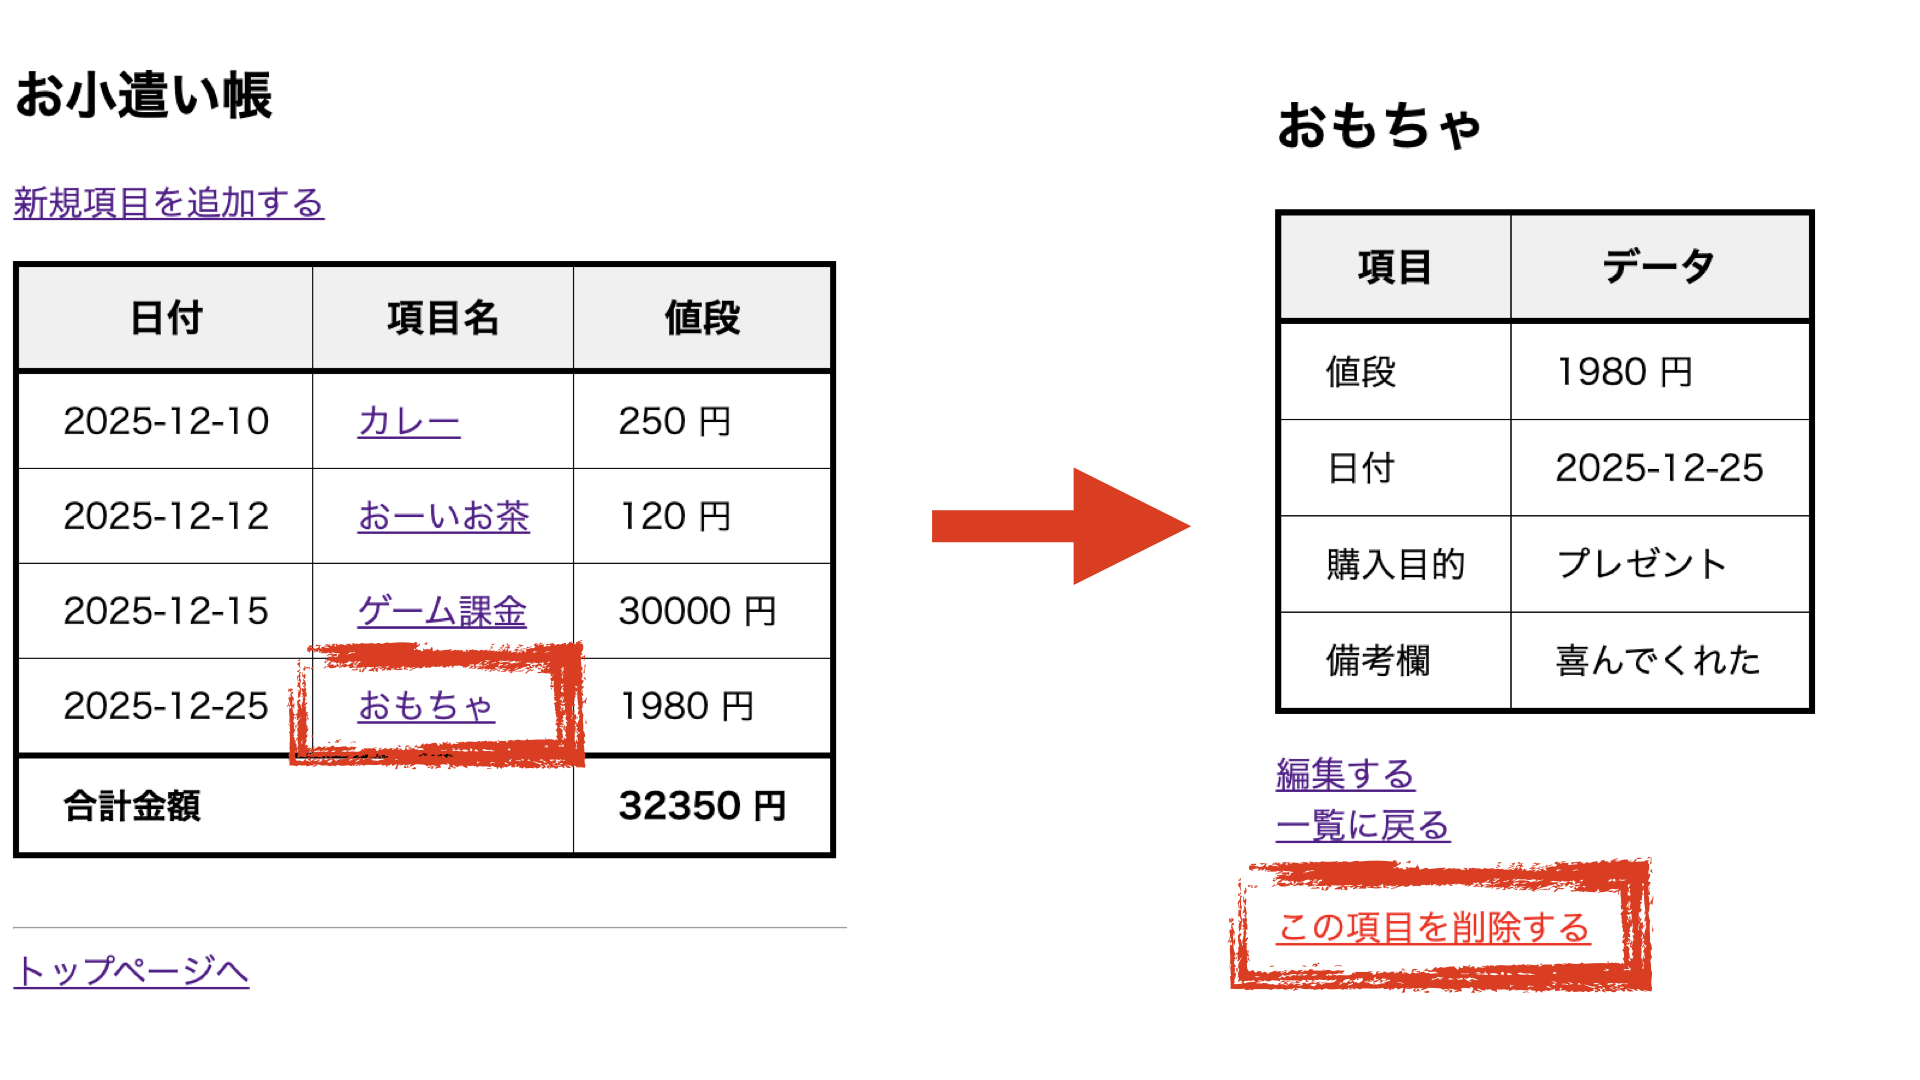
\includegraphics[width=15cm]{fig_web/wallet_go_to_delete.png}
        \caption{削除画面への行き方}
        \label{fig:go_to_delete}
        \end{center}
        \end{figure}
    \clearpage
    \item 削除確認画面が表示される（図\ref{fig:delete_confirm}）．\textbf{この操作は取り消せないため，内容をよく確認する}．削除しない場合は「キャンセル（詳細に戻る）」リンクをクリックする．
        \begin{figure}[H]
        \begin{center}
        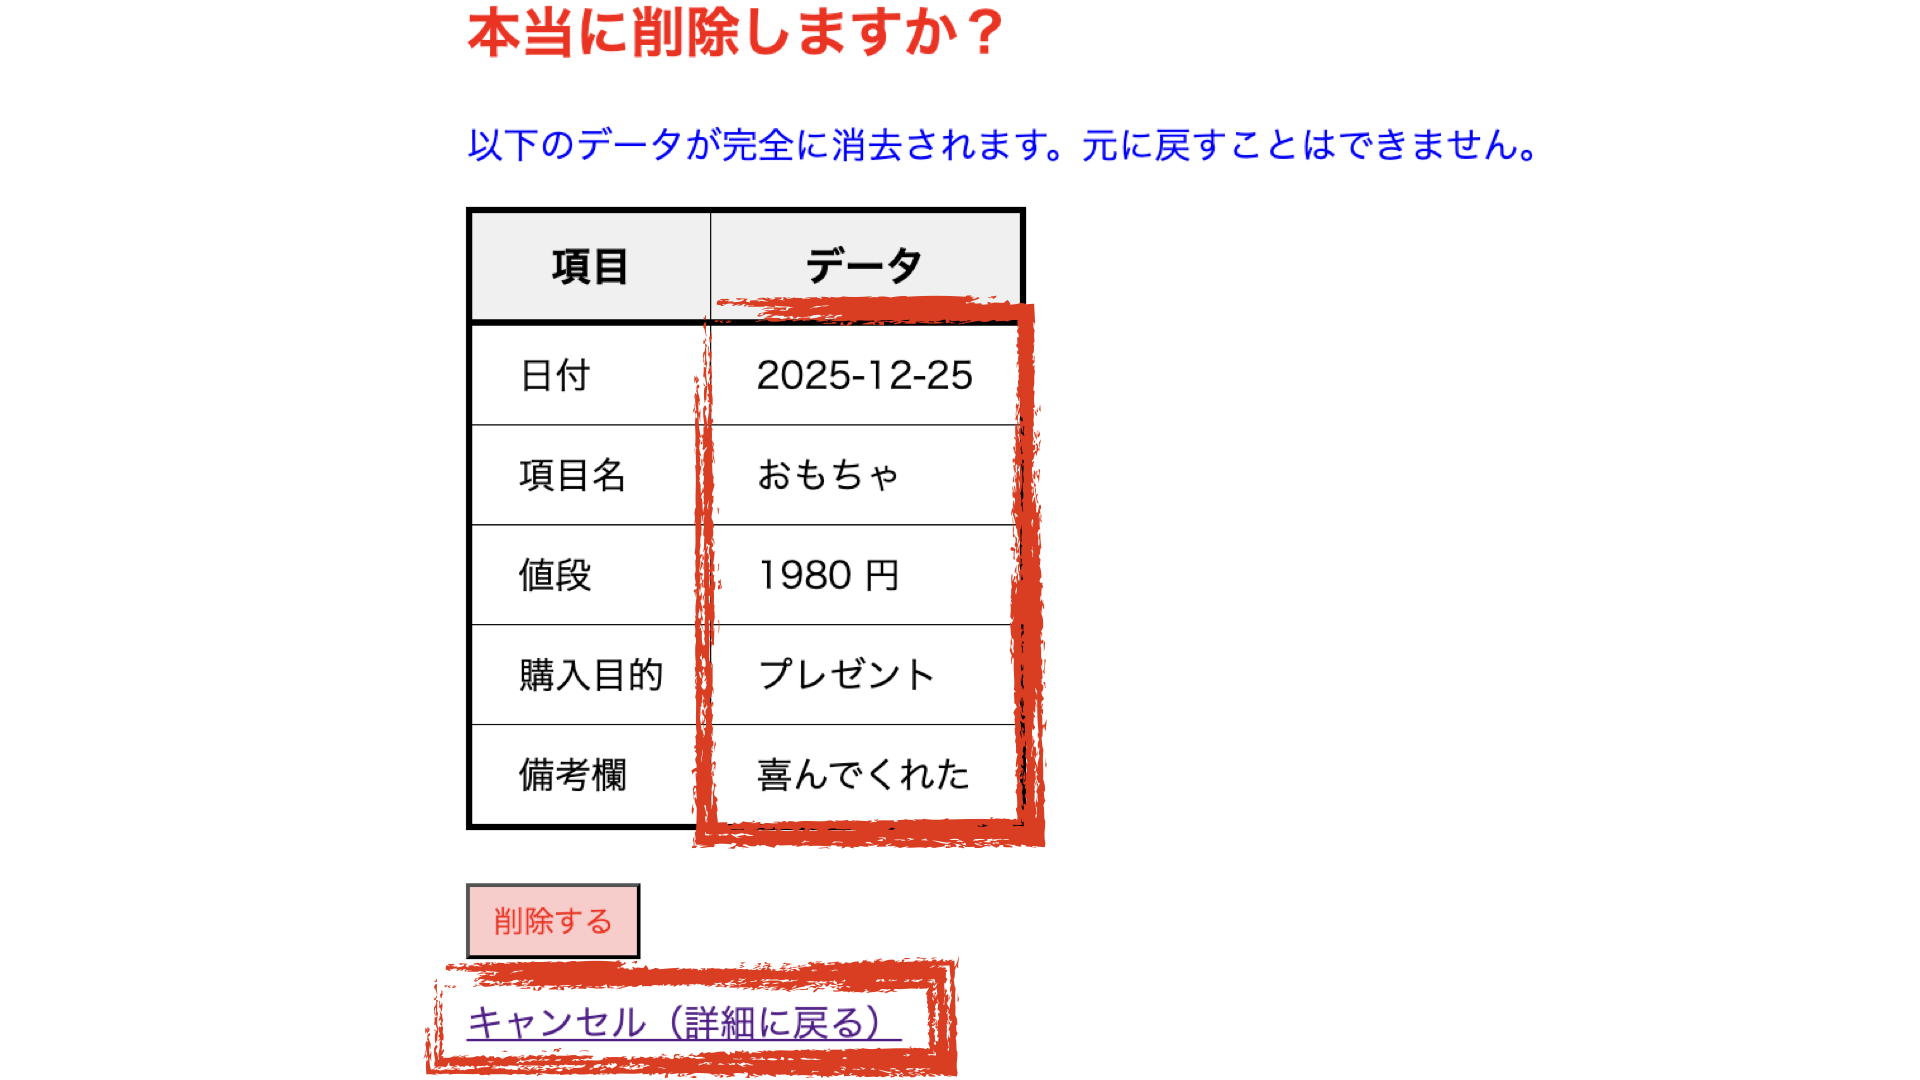
\includegraphics[width=15cm]{fig_web/wallet_delete_confirm.png}
        \caption{削除画面}
        \label{fig:delete_confirm}
        \end{center}
        \end{figure}
    \item \textbf{本当に削除してよければ}「削除する」ボタンを押す（図\ref{fig:delete}）．
        \begin{figure}[H]
        \begin{center}
        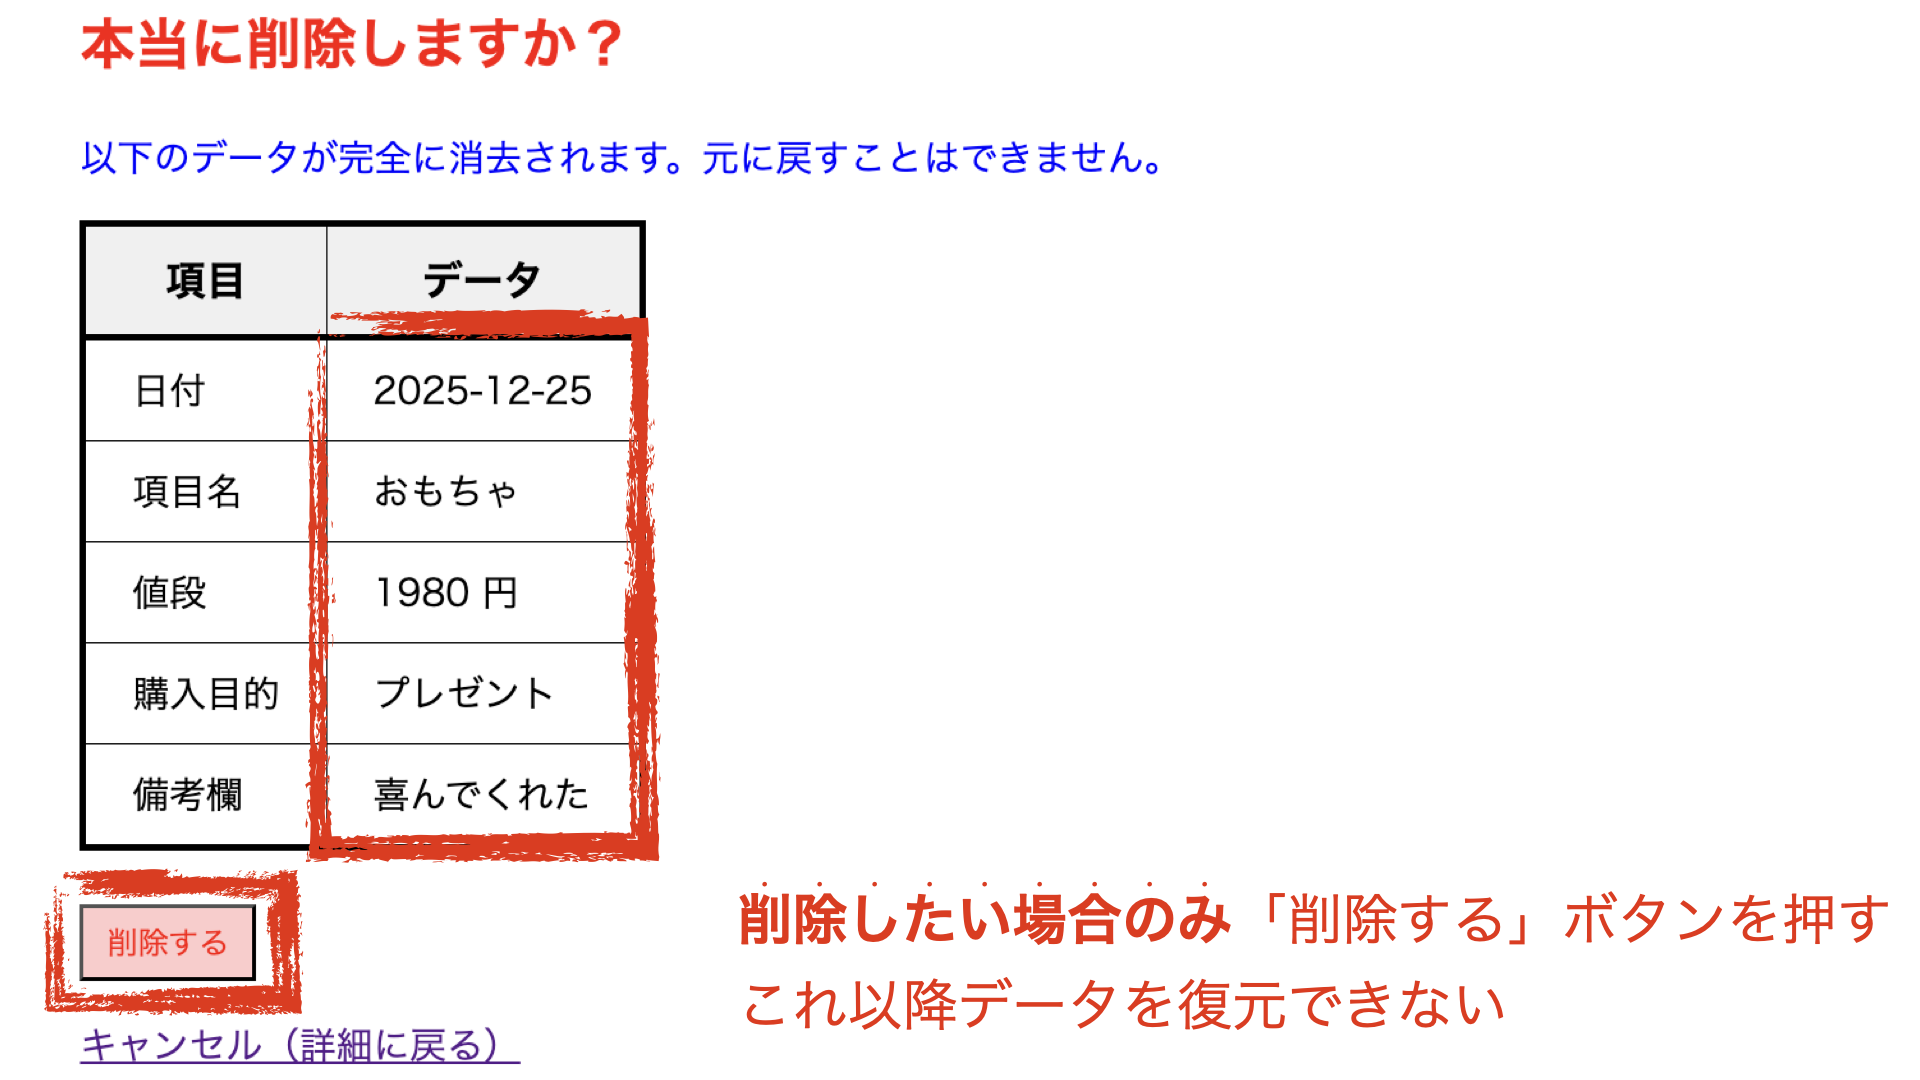
\includegraphics[width=15cm]{fig_web/wallet_delete.png}
        \caption{削除の実行}
        \label{fig:delete}
        \end{center}
        \end{figure}
    \item \textbf{本当に削除してよければ}「OK」を押す（図\ref{fig:delete2}）．これ以降，データの復元ができなくなる．削除をしない場合は「キャンセル」を押す．
        \begin{figure}[H]
        \begin{center}
        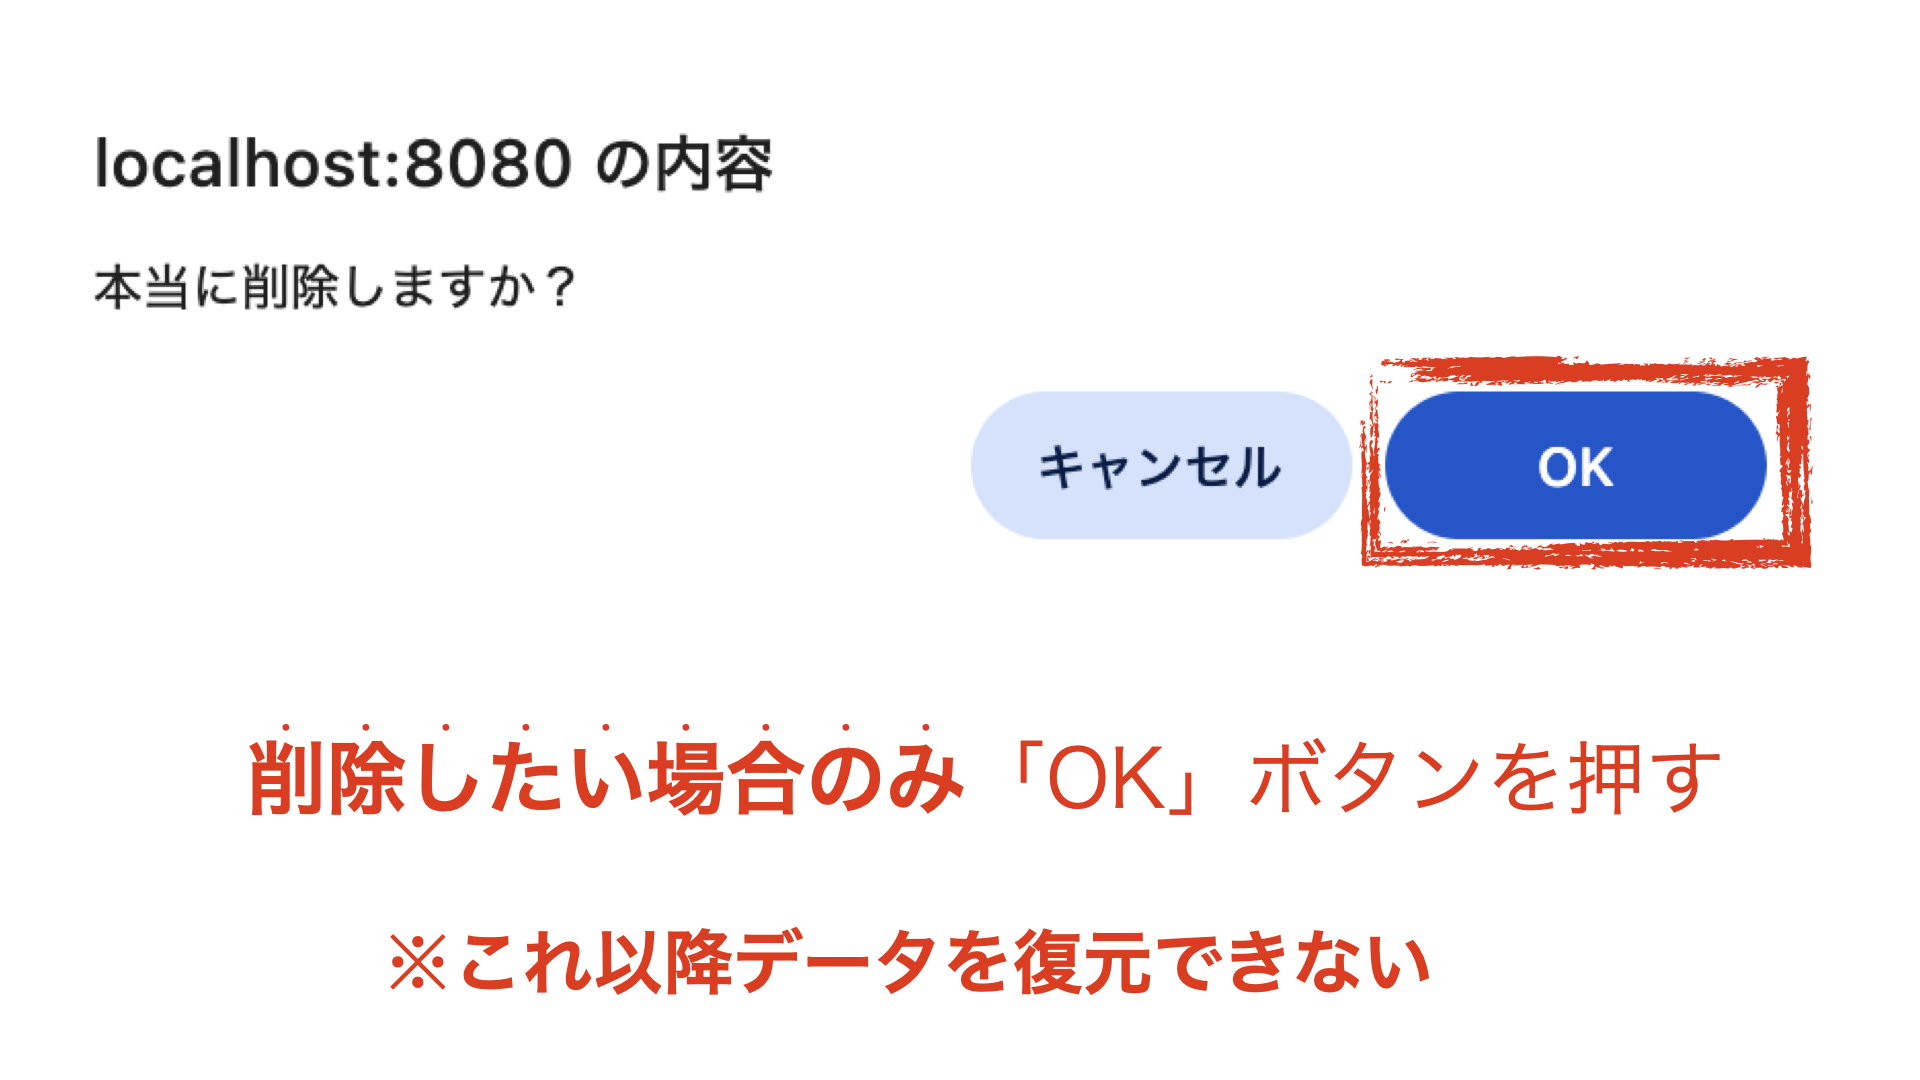
\includegraphics[width=13cm]{fig_web/wallet_delete2.png}
        \caption{削除の最終確認}
        \label{fig:delete2}
        \end{center}
        \end{figure}
    \item データが削除され，一覧画面へ戻る（図\ref{fig:delete_fin}）．一覧表示画面からは削除した項目が無くなっている．
        \begin{figure}[H]
        \begin{center}
        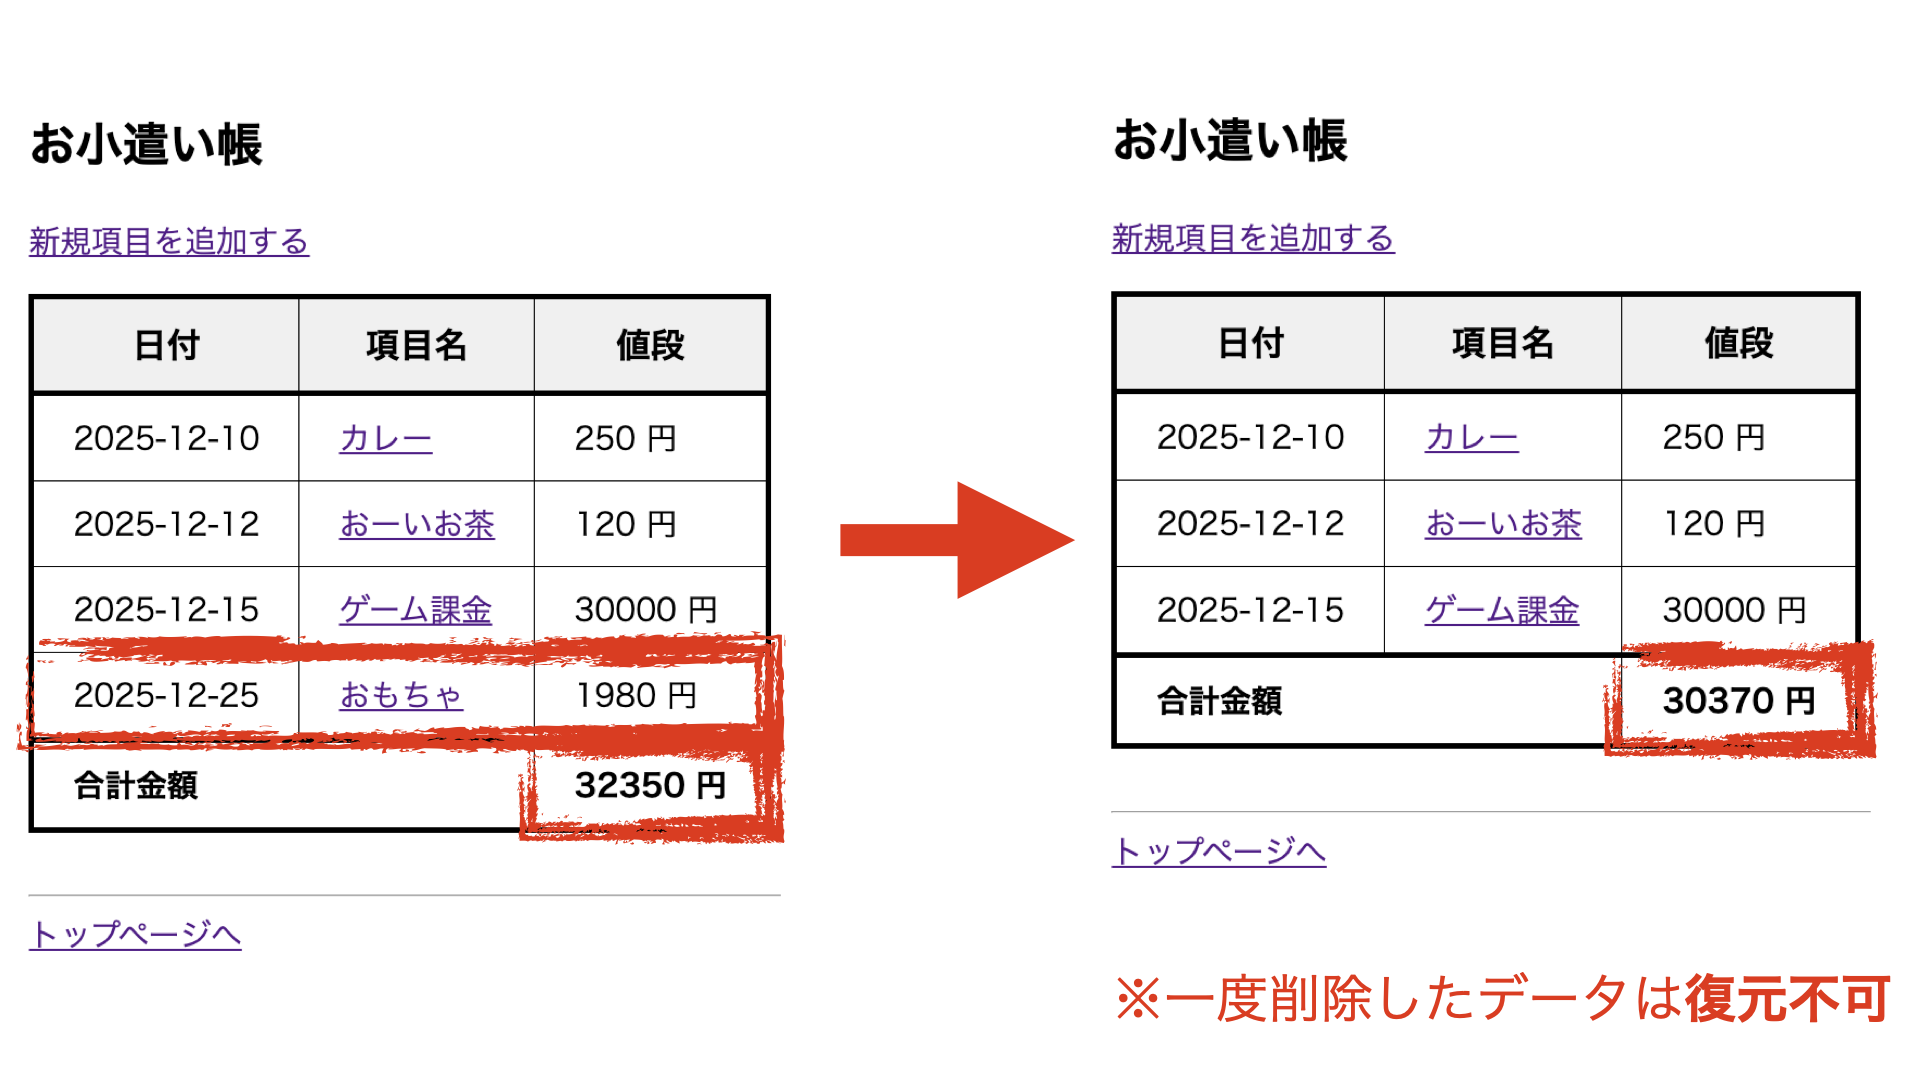
\includegraphics[width=15cm]{fig_web/wallet_delete_fin.png}
        \caption{削除後の一覧表示画面}
        \label{fig:delete_fin}
        \end{center}
        \end{figure}
\end{enumerate}



\section{管理者向けドキュメント}
\subsection{インストール方法}
\subsubsection{システム本体の準備}
本システムのソースコードはGitHubにて公開されている．GitHubのURL（\url{https://github.com/Kuro-aletta/webpro_06}）からリポジトリをダウンロード，またはターミナル上でソースコード\ref{cmd:clone}を実行し，任意のディレクトリに配置する．
\begin{lstlisting}[caption=システム本体のクローン, label=cmd:clone]
$ git clone https://github.com/Kuro-aletta/webpro_06.git
\end{lstlisting}

\subsubsection{ライブラリのインストール}
本システムはNode.js上で動作し，ExpressおよびEJSパッケージを使用する．
ターミナルを開き，システムを配置したディレクトリへ移動した後，ソースコード\ref{cmd:install}のコマンドを実行して必要なライブラリをインストールする．

\begin{lstlisting}[caption=ライブラリのインストール, label=cmd:install]
$ npm install
\end{lstlisting}
これにより，\texttt{package.json} に記載されている，本システムの実行に必要なライブラリ（express, ejs）がまとめてインストールされる．

\subsection{起動方法}
ディレクトリ内に \texttt{app\_report.js} および \texttt{node\_modules} フォルダが存在することを確認する．
確認後，ソースコード\ref{cmd:start}のコマンドを実行してサーバを起動する．
\begin{lstlisting}[caption=システムの起動, label=cmd:start]
$ node app_report.js
\end{lstlisting}
「Example app listening on port 8080!」と表示されれば起動成功である．
Webブラウザで以下のURLにアクセスして動作を確認する．
\begin{itemize}
    \item トップページ: \url{http://localhost:8080/}
    \item 成績管理システム: \url{http://localhost:8080/result}
    \item 教員情報システム: \url{http://localhost:8080/teacher}
    \item お小遣い帳システム: \url{http://localhost:8080/wallet}
\end{itemize}

\subsection{起動できない場合}
\subsubsection{ライブラリが見つからない場合}
起動時に \texttt{Error: Cannot find module 'express'} と表示される場合は，ライブラリのインストールが行われていない．\texttt{npm install} コマンド（ソースコード\ref{cmd:install}）を再度実行することで解決する．

\subsubsection{ポート番号が既に使用されている場合}
起動時に \texttt{Error: listen EADDRINUSE: address already in use :::8080} と表示される場合は，既に別のプロセスが8080番ポートを使用している．
これは多くの場合，前回のサーバ起動時に正しく終了できず，バックグラウンドでプロセスが動作し続けていることに起因する．
この場合，以下の手順でプロセスを特定し，停止させる必要がある．

\begin{enumerate}
    \item ポート8080を使用しているプロセスのID（PID）を特定する（ソースコード\ref{cmd:lsof}）．
\begin{lstlisting}[caption=PIDの確認, label=cmd:lsof]
$ lsof -i :8080
\end{lstlisting}
    \item 表示されたPID（数値）を指定してプロセスを終了（kill）する（ソースコード\ref{cmd:kill}）．
\begin{lstlisting}[caption=プロセスの終了, label=cmd:kill]
$ kill <PID>
\end{lstlisting}
    \item 上記コマンド（ソースコード\ref{cmd:kill}）でも終了しない（強制終了が必要な）場合は，\texttt{-9} を付けて再度実行する（ソースコード\ref{cmd:kill9}）．
\begin{lstlisting}[caption=プロセスの強制終了, label=cmd:kill9]
$ kill -9 <PID>
\end{lstlisting}
\end{enumerate}

なお，\texttt{app\_report.js} 内のポート番号設定（\texttt{app.listen(8080, ...)} の部分）を別の番号（8081など）に書き換えることでも対応可能であるが，アクセスするURLが変更となり利用者への周知が必要となるため，この方法は推奨しない．

\subsection{終了方法}
サーバを停止させる場合は，起動しているターミナル上で \texttt{Ctrl + C} キーを入力する．
なお，\texttt{Ctrl + Z} はプロセスを一時停止させる操作であり，完全に終了しない．この状態でターミナルを閉じるとポートが占有されたままとなり，次回の起動時にエラー（EADDRINUSE）の原因となるため注意が必要である．

\subsection{分かっている不具合・制限事項}
本システムはデータをサーバのメモリ上に保存しているため，サーバを再起動または終了すると，登録したデータはすべてリセットされる仕様である．
なお，現在確認されている動作上の不具合はない．




\section{開発者向けドキュメント}
\subsection{概要}
本システムは，サーバサイドJavaScript実行環境であるNode.jsおよびWebフレームワークExpressを用いて構築されたWebアプリケーションである．
アーキテクチャとしてMVC（Model-View-Controller）モデルに近い構成を採用しており，\texttt{views} ディレクトリ内のEJSテンプレート（View）と，\texttt{app\_report.js} によるルーティングおよびロジック処理（Controller）により動作する．
なお，本システムではデータベースを使用せず，サーバメモリ上の変数（配列）としてデータを管理する（Model相当）仕様としている．

\subsection{開発環境}
本システムの開発および動作環境は以下の通りである．
\begin{itemize}
    \item 実行環境: Node.js (v24.3.0)
    \item 言語: JavaScript
    \item フレームワーク: Express
    \item テンプレートエンジン: EJS
\end{itemize}

\subsection{ディレクトリ構造}
GitHub（\url{https://github.com/Kuro-aletta/webpro_06}）にて公開されている本システムのファイル構成を図\ref{fig:dir_tree}に示す．なお，本システムに関与しないファイルは省略されている．
実行の起点となるプログラムである \texttt{app\_report.js} をルートに置き，静的リソース（CSSなど）は \texttt{public} ディレクトリ，画面のひな型となるEJSファイルは \texttt{views} ディレクトリに配置して管理している．

\begin{figure}[H]
\renewcommand*\DTstylecomment{\rmfamily\color{black}\footnotesize\itshape} % コメントのスタイル調整（任意）
\dirtree{%
.1 webpro\_06/.
.2 app\_report.js \DTcomment{サーバサイドプログラム}.
.2 package.json \DTcomment{依存ライブラリ定義}.
.2 node\_modules/ \DTcomment{インストールされたライブラリ}.
.2 public/ \DTcomment{静的ファイル用ディレクトリ}.
.3 style.css \DTcomment{共通スタイルシート}.
.3 top.html \DTcomment{トップページ}.
.2 views/ \DTcomment{EJSファイル用ディレクトリ}.
.3 result\_list.ejs \DTcomment{成績:一覧}.
.3 result\_detail.ejs \DTcomment{成績:詳細}.
.3 result\_add.ejs \DTcomment{成績:追加入力}.
.3 result\_add\_confirm.ejs \DTcomment{成績:追加確認}.
.3 result\_edit.ejs \DTcomment{成績:編集入力}.
.3 result\_edit\_confirm.ejs \DTcomment{成績:編集確認}.
.3 result\_delete\_confirm.ejs \DTcomment{成績:削除確認}.
.3 teacher\_list.ejs \DTcomment{教員:一覧}.
.3 teacher\_detail.ejs \DTcomment{教員:詳細}.
.3 teacher\_add.ejs \DTcomment{教員:追加入力}.
.3 teacher\_add\_confirm.ejs \DTcomment{教員:追加確認}.
.3 teacher\_edit.ejs \DTcomment{教員:編集入力}.
.3 teacher\_edit\_confirm.ejs \DTcomment{教員:編集確認}.
.3 teacher\_delete\_confirm.ejs \DTcomment{教員:削除確認}.
.3 wallet\_list.ejs \DTcomment{財布:一覧}.
.3 wallet\_detail.ejs \DTcomment{財布:詳細}.
.3 wallet\_add.ejs \DTcomment{財布:追加入力}.
.3 wallet\_add\_confirm.ejs \DTcomment{財布:追加確認}.
.3 wallet\_edit.ejs \DTcomment{財布:編集入力}.
.3 wallet\_edit\_confirm.ejs \DTcomment{財布:編集確認}.
.3 wallet\_delete\_confirm.ejs \DTcomment{財布:削除確認}.
}
\caption{ディレクトリ構造}
\label{fig:dir_tree}
\end{figure}

\subsection{システム構造とURL設計}
本システムは，\texttt{app\_report.js} を実行し，\texttt{views/} ディレクトリ内のEJSファイルをもとにHTMLを生成して表示する構成をとっている．
データの永続化は行わず，サーバメモリ上の変数（配列）としてデータを保持する仕様とした．

各システムにおけるページ遷移図を図\ref{fig:md}に，HTTPメソッド，リソース名（URL）の対応を表\ref{tab:url}に示す．
\begin{figure}[H]
 \begin{center}
  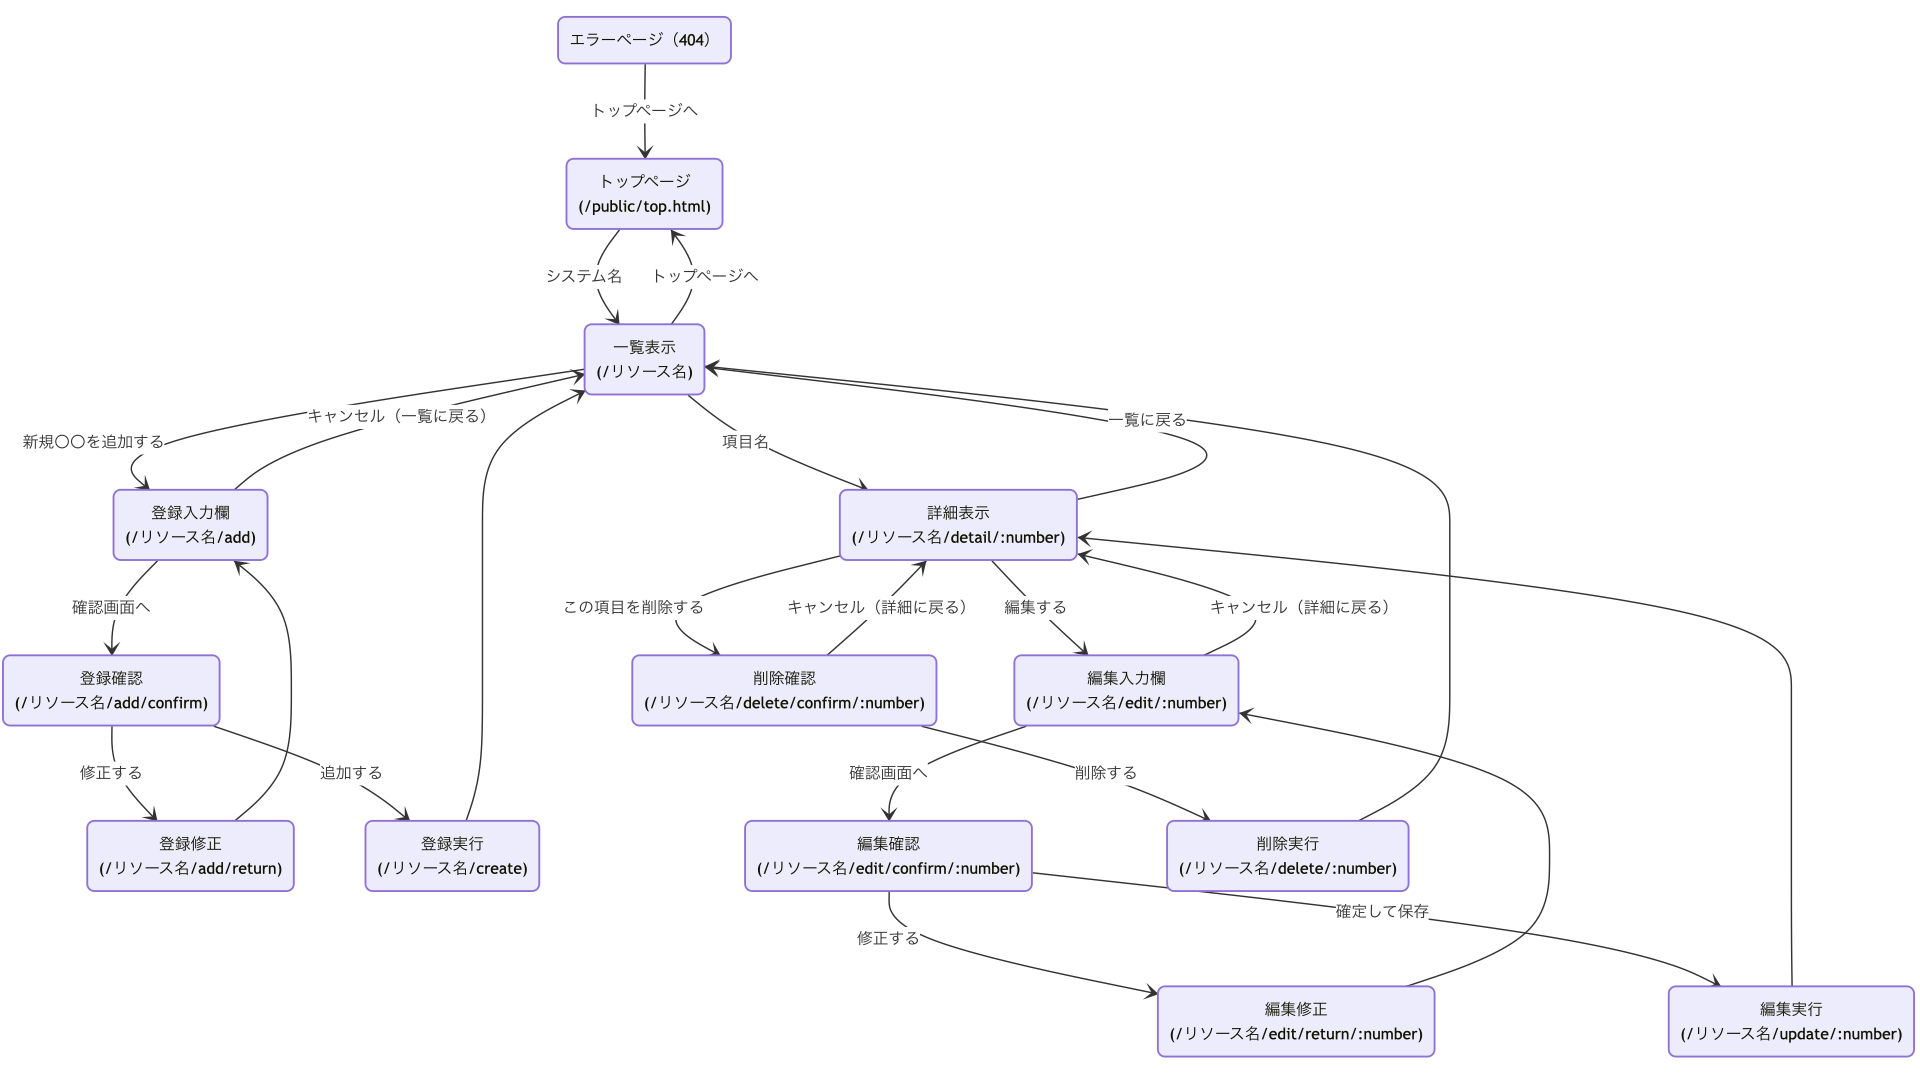
\includegraphics[width=1\linewidth]{fig_web/md.png}
  \caption{ページ遷移図}
  \label{fig:md}
 \end{center}
\end{figure}
\begin{table}[H]
\caption{URL設計とHTTPメソッド}
\label{tab:url}
\centering
\begin{tabular}{l|l|l}
\hline
画面・機能 & HTTPメソッド & URLパターン \\
\hline \hline
トップページ & GET & \texttt{/} \\
\hline
一覧表示 & GET & \texttt{/リソース名} \\
詳細表示 & GET & \texttt{/リソース名/detail/:number} \\
新規登録（入力） & GET & \texttt{/リソース名/add} \\
新規登録（確認） & POST & \texttt{/リソース名/add/confirm} \\
新規登録（修正） & POST & \texttt{/リソース名/add/return} \\
新規登録（実行） & POST & \texttt{/リソース名/create} \\
編集（入力） & GET & \texttt{/リソース名/edit/:number} \\
編集（確認） & POST & \texttt{/リソース名/edit/confirm/:number} \\
編集（修正） & POST & \texttt{/リソース名/edit/return/:number} \\
編集（実行） & POST & \texttt{/リソース名/update/:number} \\
削除（確認） & GET & \texttt{/リソース名/delete/confirm/:number} \\
削除（実行） & POST & \texttt{/リソース名/delete/:number} \\
\hline
エラー（404） & ALL & - \\
\hline
\end{tabular}
\end{table}
\clearpage
各システムのリソース名は以下の通りである．
\begin{itemize}
    \item 成績管理システム: \texttt{result}
    \item 教員情報システム: \texttt{teacher}
    \item お小遣い帳システム: \texttt{wallet}
\end{itemize}

以下に，本システムの画面遷移やデータの受け渡しに関する詳細な仕組みを述べる．

\subsubsection{ページ遷移の仕組み}
各画面間の遷移は，主に以下の2つの方法で行われる．
\begin{itemize}
    \item \textbf{参照（GET）}: 一覧画面の各項目やメニューのリンク（\texttt{<a>}タグ）をクリックすることで遷移する．
    \item \textbf{操作（POST）}: 登録・編集・削除の確認画面や実行処理へは，フォーム（\texttt{<form>}タグ）の送信ボタンをクリックすることで遷移する．
\end{itemize}

\subsubsection{データの受け渡し（リレー方式）}
新規登録や編集の際，入力画面から確認画面を経て実行処理へと進む過程で，一度サーバに送信したデータを維持する必要がある．
本システムでは，HTTPの直前の状態を保持しない特性を補うため，確認画面のフォーム内に \texttt{type="hidden"} 属性を持つ \texttt{input} タグを配置し，次画面へ再度データを送信して受け渡す「リレー方式」を採用した．

\subsubsection{処理実行後の画面遷移}
データの追加・更新・削除が完了した後の遷移先は，ユーザビリティを考慮して以下のように設計した．
\begin{itemize}
    \item \textbf{追加・削除後}: 作業結果全体を確認しやすくするため，「一覧表示画面」へリダイレクトする．
    \item \textbf{編集後}: 変更内容を即座に確認できるようにするため，そのデータの「詳細表示画面」へリダイレクトする．
\end{itemize}

\clearpage
\subsection{データ構造}
各システムは，オブジェクトの配列としてデータを管理している．それぞれのデータ構造を以下に示す．

\subsubsection{成績管理システム (result)}
履修科目の成績情報を管理する．
\begin{table}[H]
\caption{成績データの構造}
\centering
\begin{tabular}{l|l|l}
\hline
項目名 & 変数名 & 説明 \\
\hline \hline
年度 & year & 開講年度（数値） \\
セメスタ & semester & 開講学期（数値） \\
科目名 & name & 講義の名称 \\
担当教員 & teacher & 教員名 \\
副担当 & subteacher & 副担当教員名（任意） \\
単位数 & credit & 科目の単位数（数値） \\
成績 & grade & S, A, B, C, 合 など \\
\hline
\end{tabular}
\end{table}

\subsubsection{教員情報システム (teacher)}
教員の所属や担当科目などの情報を管理する．
\begin{table}[H]
\caption{教員データの構造}
\centering
\begin{tabular}{l|l|l}
\hline
項目名 & 変数名 & 説明 \\
\hline \hline
学科 & department & 所属学科名 \\
氏名 & name & 教員名 \\
職位 & job & 教授，准教授など \\
研究室 & laboratory & 研究室名 \\
担当科目 & subject & 主な担当科目 \\
\hline
\end{tabular}
\end{table}

\subsubsection{お小遣い帳システム (wallet)}
金銭の出納記録を管理する．合計金額の計算に使用するため，\texttt{price} は必ず数値型として扱う．
\begin{table}[H]
\caption{お小遣い帳データの構造}
\centering
\begin{tabular}{l|l|l}
\hline
項目名 & 変数名 & 説明 \\
\hline \hline
日付 & date & 利用日（YYYY-MM-DD形式） \\
項目名 & item & 購入品目などの名称 \\
値段 & price & 金額（数値） \\
購入目的 & purpose & 利用の目的 \\
備考欄 & memo & メモ \\
\hline
\end{tabular}
\end{table}

\subsection{各システムの機能詳細}
\subsubsection{成績管理システム}
履修データの登録・編集・削除を行う．
一覧画面では，科目名(\texttt{name})をクリックすることで詳細画面へ遷移する．教員名が未入力の場合は「（科目名を設定してください）」と表示することで，詳細画面へ遷移できなくなる状況を防いでいる．
表示制御として，成績(\texttt{grade})が未入力の場合には「 - 」を，科目名が未入力の場合には注意書きとして「（科目名を設定してください）」を表示するようにしている．
詳細画面においては，副担当教員(\texttt{subteacher})が登録されていない（空文字の）場合，テーブルの行自体を表示しないようにしている．また，成績(\texttt{grade})が未入力の場合には「未評価」を表示するようにしている．

\subsubsection{教員情報システム}
教員データの管理を行う．
一覧画面では，教員名(\texttt{name})をクリックすることで詳細画面へ遷移する．教員名が未入力の場合は「（教員名を設定してください）」と表示することで，詳細画面へ遷移できなくなる状況を防いでいる．
詳細画面では，担当科目(\texttt{subject})が登録されていない場合に「なし」と表示する処理を加えている．

\subsubsection{お小遣い帳システム}
支出データの管理を行う．
一覧画面では，項目名(\texttt{item})をクリックすることで詳細画面へ遷移する．項目名が未入力の場合は警告として「（項目名を設定してください）」を表示することで，詳細画面へ遷移できなくなる状況を防いでいる．
本システム特有の機能として，一覧表示を行う際，サーバ側で登録済みデータの値段(\texttt{price})をすべて加算し，合計金額を算出する処理を実装している．算出された合計値は一覧表の最下部に表示される．

\subsection{講義範囲外の要素の実装}
本システムの開発にあたり，ユーザビリティの向上やデータの整合性を保つため，いくつかの工夫を取り入れた．

\subsubsection{EJS内での条件分岐 (if文)}
\texttt{result\_list.ejs} などにおいて，データが空文字の場合の表示を制御するためにEJS内でif文を使用した．
例えば，成績が空の場合は「 - 」を表示し，入力済みの場合はそのままを表示することで，視認性を向上させている．

\begin{lstlisting}[caption=EJSでの条件分岐の例]
<% if (row.grade == "") { %>
  -
<% } else { %>
  <%= row.grade %>
<% } %>
\end{lstlisting}

\subsubsection{CSSによるデザインの管理}
本システムでは，画面の見た目（デザイン）をHTMLファイル（.ejs）から分離し，一括管理するためにCSS（Cascading Style Sheets）を導入した．
\texttt{public} フォルダに \texttt{style.css} ファイルを作成し，各EJSファイルから \texttt{<link>} タグを用いて読み込んでいる．
これにより，HTML内に \texttt{border="3"} などの属性を記述することなく，全ページで統一されたデザインを適用している．
今回実装した主なCSSの機能を表\ref{tab:css}に示す．

\begin{table}[H]
\caption{定義したCSSクラスとスタイル}
\label{tab:css}
\centering
\begin{tabular}{l|l|l}
\hline
セレクタ/クラス名 & 対象の要素 & 機能・効果 \\
\hline \hline
\texttt{table} & \texttt{<table>} & 外枠を3pxの実線にし，枠線を結合する \\
\texttt{th} & \texttt{<th>} & 背景色を灰色にし，文字を拡大，下線を太くする \\
\texttt{td} & \texttt{<td>} & 内側の枠線を1pxにし，余白（padding）を設ける \\
\texttt{.text-red} & クラス指定 & 文字色を赤にする（削除確認メッセージ等） \\
\texttt{.text-blue} & クラス指定 & 文字色を青にする（登録確認メッセージ等） \\
\texttt{.delete} & クラス指定 & 背景色を薄い赤にする（削除ボタン用） \\
\texttt{input[type="submit"]} & 送信ボタン & 余白を設け，カーソルを指の形にする \\
\texttt{.total-border} & クラス指定 & 上線を3pxの実線にする（合計金額欄用） \\
\hline
\end{tabular}
\end{table}

EJSファイル側では，ソースコード\ref{ex1}のように \texttt{class} 属性を指定して，CSSで定義したスタイルを適用している．

\begin{lstlisting}[caption=CSSクラスの適用例, label=ex1]
<h2 class="text-red">まだ保存されていません</h2>

<td class="total-border">合計金額</td>
\end{lstlisting}

\subsubsection{入力補助のためのsmallタグ}
新規登録や編集画面において，入力項目の下に \texttt{<small>} タグを用いて注釈（例：「※半角数字で入力」など）を追加した．これにより，ユーザが期待されるデータ形式を直感的に理解できるようにした．

\subsubsection{数値計算と入力値の検証}
お小遣い帳システムにおいて，フォームから送信されたデータは通常「文字列」としてサーバに受け渡される．
そのままでは正しい加算処理（合計金額の算出）ができないため，ソースコード\ref{ex2}のように，データの登録時および更新時にJavaScriptの \texttt{parseInt()} 関数を使用して明示的に整数型へ変換して保存する処理を実装した．
また，金額が未入力（空文字）の場合に計算結果が \texttt{NaN}（非数値）になるのを防ぐため，\texttt{isNaN()} 関数を用いた入力値のチェックを行い，数値でない場合は0として扱うよう堅牢性を高めた．

\begin{lstlisting}[caption=数値変換と検証の処理, label=ex2]
// フォームからの入力を数値に変換
let priceVal = parseInt(req.body.price);

// 数値でない場合（空欄など）は0にする
if (isNaN(priceVal)) {
    priceVal = 0;
}
\end{lstlisting}

\subsubsection{JavaScript による送信確認アラート}
誤操作によるデータの削除を防ぐため，ソースコード\ref{src:js_confirm}のように，削除実行ボタンに JavaScript の \texttt{confirm()} メソッドを組み込んだ．
これにより，ボタンクリック時にブラウザ標準の確認ダイアログが表示され，ユーザが「OK」を選択した場合のみ処理が実行され，「キャンセル」を選択した場合は処理が中断される安全な仕様とした．

\begin{lstlisting}[caption=削除ボタンへの確認アラート実装, label=src:js_confirm]
<input type="submit" value="削除する" class="delete"
       onclick="return confirm('本当に削除しますか？');">
\end{lstlisting}



\section{おわりに}
本レポートでは，成績管理，教員情報，お小遣い帳という3つのWebアプリケーションの設計と実装について報告した．
統一された操作体系を持つシステムを複数構築することで，Web開発における共通のパターンを深く理解することができた．

本課題を通じて，Webアプリケーションにおける基本的なCRUD操作の実装方法を習得した．
特に，データの更新や削除といったデータの変更を伴う操作にはPOSTメソッドを使用し，単なる参照にはGETメソッドを使用するというWebの標準的な設計ルールの重要性を理解した．
また，確認画面を挟む実装においては，一度サーバにデータを送信した後，\texttt{hidden} 属性を用いて再度データを次の画面へ受け渡すリレー方式を採用した．これにより，通信のたびに接続が切れる（直前の状態を保持しない）HTTPの特性において，画面間でデータを引き継ぐ方法を学んだ．
さらに，CSSを用いて見た目のデザインとHTMLの構造を分けて管理することや，データの型を意識した入力値のチェックなど，実用的なWebシステム開発に必要な周辺技術についても理解を深めることができた．

今回はデータの保存をメモリ上の変数で行ったため，サーバ停止とともにデータがリセットされる仕様であるが，今後はデータベースを用いた永続化など，より実用的なシステムへの発展が課題である．


\end{document}
